%-----------------------------------------------------------------------------
\documentclass[12pt,a4paper]{report}
%---------------------------------------------------------------------------
\usepackage{amsmath}
\usepackage{amssymb}
\usepackage{amsthm}
% enumitem is loaded for the web build: without it tex4ht discards the
% optional label on \item[(i)] and renumbers the list itself.
\usepackage{enumitem}
\usepackage{amsfonts}
\usepackage{array}
\usepackage{longtable}
\usepackage{appendix}
\usepackage{blkarray}
\usepackage{bibentry}
\usepackage[none]{hyphenat}
\usepackage[noadjust]{cite}
\usepackage{filecontents}
\usepackage[all,knot,arc,poly]{xy}
\usepackage{graphicx}
\graphicspath{{images/}{../images/}}
\DeclareGraphicsExtensions{.pdf,.jpeg,.png, .jpg}
\usepackage{lscape}
\usepackage{epsfig}
\usepackage{mathrsfs}
\usepackage[left=40mm,right=25mm,top=25mm,bottom=25mm]{geometry}
\usepackage{url}
\usepackage{multicol}
\usepackage{multirow}
\usepackage{color}
\usepackage[table]{xcolor}
\definecolor{pink}{rgb}{1,0.5,0.5}
\usepackage{graphicx}
\graphicspath{ {images/} }
\usepackage{float}
\floatstyle{boxed} 
\restylefloat{figure}
%\usepackage[graphicx]{realboxes}
\usepackage{rotating}
%\usepackage{shadow}
%-----------------------------------------------------------------------------
\usepackage{setspace}
\usepackage{titletoc}
\titlecontents{chapter}
[0pt]
{\bfseries}
{\MakeUppercase\chaptername\ \thecontentslabel:\quad}
{\MakeUppercase}
{\hfill\contentspage}[]
%-----------------------------------------------------------------------------
\usepackage{float}
\textwidth 6.5in \textheight 9.175in\topmargin 0in \headheight 0in
\oddsidemargin 0in \evensidemargin 0in
\parskip 0.5\baselineskip
\parindent 0pt
\renewcommand{\baselinestretch}{1.25}
%-----------------------------------------------------------------------------
\theoremstyle{definition}
\newtheorem{thm}{Theorem}[section]
\newtheorem{defn}[thm]{Definition}
\newtheorem{exa}[thm]{Example}
\newtheorem{exe}[thm]{Exercise}
\newtheorem{note}[thm]{Note}
\newtheorem{remark}[thm]{Remark}
\theoremstyle{plain}
\newtheorem{prop}[thm]{Proposition}
\newtheorem{conj}[thm]{Conjecture}
\newtheorem{coro}[thm]{Corollary}
\newtheorem{lem}[thm]{Lemma}
\newtheorem{tech}{Technique}[section]
\newtheorem{fact}[thm]{Fact}
% Practice problems, numbered separately from the theorem counter so that adding
% one never renumbers a theorem the text refers to. site/build.py collapses the
% solution behind a disclosure control.
\newtheorem{problemx}{Problem}[section]
\newenvironment{problem}{\begin{problemx}}{\end{problemx}}
\newenvironment{solution}
  {\renewcommand{\qedsymbol}{}\begin{proof}[\textit{Solution}.]}
  {\end{proof}}
\renewcommand{\contentsname}{TABLE OF CONTENTS}
\renewcommand\bibname{REFERENCES}
%\renewcommand{\qedsymbol}{$\blacksquare$}

\parindent 0ex

%-----------------------------------------------------------------------------
\usepackage{titlesec}
\titleformat{\chapter}[hang]
          {\normalfont\filright\ttfamily\scshape\sffamily\bfseries
          	\centering\large}
          {\MakeUppercase{\chaptertitlename}\ \thechapter}{10pt\ :}{\large\MakeUppercase}        
          \titlespacing*{\chapter}{0pt}{-90pt}{16pt}
                       
\titleformat{\section}[hang]
           {\normalfont\sffamily\bfseries%
            \large}
            {\thesection.}{1ex}{}%[\titlerule]
%-----------------------------------------------------------------------------


%-----------------------------------------------------------------------------
\usepackage{fancyhdr}
\fancyhead{}

%-----------------------------------------------------------------------------

\renewcommand{\sectionmark}[1]{\markright{}} %\thesection\ #1 (this one should be in th brackets, ayoub)
%-----------------------------------------------------------------------------

%-----------------------------------------------------------------------------


\newcommand{\bpf}{\noindent {\ttfamily  PROOF}. $\mbox{}$}
\newcommand{\epf}{\hfill \hbox{\raisebox{.5ex}{$\blacksquare$}$\phantom{.}$}}
%-----------------------------------------------------------------------------

%-----------------------------------------------------------------------------
% tikz is loaded last: it pulls in graphicx and xcolor, and this file loads both
% itself further up. Loading tikz early makes the option processing collide and
% tex4ht fails in the preamble with an unhelpful message about \@reset@ptions.
\usepackage{tikz}
\usetikzlibrary{patterns,graphs,arrows.meta,shapes,trees,bending,fadings,quotes,angles}

\begin{document}
\pagenumbering{roman}
% Title page depersonalised for the web, as with every other course here:
% no university, no author, no year. The identity kept below is Euler's
% reflection formula, which ties the gamma function to the trigonometric
% functions and is as good a summary of the course as a subtitle would be.
\begin{titlepage}
\begin{center}
\vspace*{3cm}
{\Huge\bfseries Topics in Mathematical Methods}\\[1.2cm]
{\large Lecture Notes}\\[2.5cm]
\line(1,0){300}\\[1.5cm]
$$\Gamma(z)\,\Gamma(1-z) \;=\; \frac{\pi}{\sin \pi z},
\qquad 0 < \operatorname{Re} z < 1$$
\end{center}
\end{titlepage}
%\maketitle












%----------------------------------------------------------------------------------------------------------------------------------------------------

\newpage
%\phantom{.}
%\vspace{20mm}
%\noindent
%Table of contents
\begin{spacing}{1.7}
\tableofcontents
\addcontentsline{toc}{chapter}{TABLE of CONTENTS}
\end{spacing}

\newpage
%\noindent
%\begin{center}
%{\Large\bf Index of Notation} 
%\end{center}

















\newpage
\pagenumbering{arabic}


%--------------------------------------------------------------------------------------------------------------------------------





     
%-------------------------------------------------------------------------------------------------------------------------------------------------------
\chapter{Improper Integrals}
\vspace*{-7mm}
We wish to discuss topics which have varied applications in mathematical analysis. Particularly, we shall consider various special functions, some of which are solutions of certain \textit{Differential Equations}. Since most special functions occur as improper integrals, we first review the concept of improper integrals.



\section{Improper Integrals of the First Kind}
An integral of the form $$\int_a^{\infty} f(x)\, dx$$ in which $f(x)$ is defined for $x\geq a$ and integrable over every finite interval $[a,b]$ is said to be of the first kind. \\
We then have $$\int_a^{\infty}f(x)\, dx = \lim_{b\rightarrow\infty}\int_a^bf(x)\, dx.$$
If the limit exits we say that the improper integral is convergent, otherwise it is said to be divergent.


If the function $f$ is continuous on the whole real line, we define
$$\int_{-\infty}^{\infty}f(x)\, dx = \int_{-\infty}^cf(x)\, dx + \int_c^{\infty} f(x)\, dx$$
for any convenient choice of $c$, provided the two integrals on the right hand side both converge.


Note that the choice of $c$ above does not matter. For, if $c<d$
\begin{align*}
\int_{-\infty}^cf(x)\, dx + \int_c^{\infty}f(x)\, dx & = \int_{-\infty}^cf(x)\, dx + \int_c^df(x)\, dx + \int_d^{\infty}f(x)\, dx\\
                                            & = \int^d_{-\infty}f(x)\, dx + \int_d^{\infty}f(x)\, dx.
\end{align*}

Also we immediately observe that
$$\int_{-\infty}^{\infty}f(x)\, dx \neq \lim_{t\rightarrow \infty} \int^t_{-t} f(x)\, dx.$$





\begin{exa}
Show that $$\int_{-\infty}^{\infty} \frac{1 + x}{1 + x^2}\, dx$$ diverges, but that $$\lim_{t\rightarrow\infty}\int_{-t}^{t} \frac{1 + x}{1 + x^2}\, dx = \pi .$$
\end{exa}


\begin{proof}[Working]
First consider the indefinite integral 
\begin{align*}
\int \frac{1 + x}{1 + x^2}\, dx & = \int \frac{1}{1 + x^2}\, dx + \int\frac{x}{1 + x^2}\, dx\\  
& = \tan^{-1}x + \frac{1}{2}\ln (1 + x^2) + c.
\end{align*}
Now
\begin{align*}
\int^{\infty}_{-\infty} \frac{1 + x}{1 + x^2}\,\, dx & = \int^{\infty}_{c} \frac{1 + x}{1 + x^2}\, dx + \int^{c}_{-\infty} \frac{1 + x}{1 + x^2}\, dx\\\\
& = \lim_{t\rightarrow \infty}\int^{t}_{c} \frac{1 + x}{1 + x^2}\, dx + \lim_{t\rightarrow \infty}\int^{c}_{-t} \frac{1 + x}{1 + x^2}\, dx\\
& = \infty - \infty, 
\end{align*}
so the integral diverges.

However, 
\begin{align*}
\lim_{t\rightarrow \infty} \int_{-t}^t \frac{1 + x}{1 + x^2}\, dx & = \lim_{t\rightarrow \infty}\left[\tan^{-1}x + \frac{1}{2} \ln (1 + x^2) \right]_{-t}^t\\
& = \lim_{t\rightarrow \infty}\left[\tan^{-1}(t) - \tan^{-1}(-t)\right]\\
& = \frac{\pi}{2} - \left(\frac{-\pi}{2}\right)\\
& = \pi.
\end{align*}
\end{proof}





\begin{exa}
Investigate the improper integrals
\begin{multicols}{3}
\begin{enumerate}
\item[(a).] $\displaystyle{\int_1^{\infty} \frac{1}{x^2}\, dx}$
\item[(b).] $\displaystyle{\int_1^{\infty}\frac{1}{x}\, dx}$
\item[(c).] $\displaystyle{\int_{-\infty}^0\frac{1}{\sqrt{1 - x}}\, dx}$
\end{enumerate}
\end{multicols}
\end{exa}


\begin{proof}[Working]
\begin{enumerate}
\item[(a).] $$\int^{\infty}_1\frac{1}{x^2}\, dx  = \lim_{t\rightarrow \infty} \int_1^t\frac{1}{x^2}\, dx  = \lim_{t\rightarrow \infty}\left[-\frac{1}{x}\right]_1^t = \lim_{t\rightarrow \infty}\left[-\frac{1}{t} + 1\right] = 1.$$ So the integral converges.


\item[(b).] $$\int_1^{\infty}\frac{1}{x}\, dx = \lim_{t\rightarrow \infty} \int_1^t\frac{1}{x}\, dx = \lim_{t\rightarrow \infty} \left[\ln |x|\right]_1^t = \lim_{t\rightarrow \infty}[\ln t - \ln 1] = \infty,$$
so the integral diverges.


\item[(c).] $$\int_{-\infty}^0\frac{1}{\sqrt{1 - x}}\, dx = \lim_{t\rightarrow -\infty}\int_t^0\frac{1}{\sqrt{1 - x}}\, dx = \lim_{t\rightarrow -\infty}\left[-2\sqrt{1 - x}\right]_t^0 = \infty,$$
diverges.
\end{enumerate}
\end{proof}



\begin{exa}[\textit{$p$-Integrals}]
For what values of $p$ is the integral $$\int_1^{\infty}\frac{1}{x^p}\, dx$$ convergent?
\end{exa}

\begin{proof}[Working]
$$\int_1^{\infty}\frac{1}{x^p}\, dx = \lim_{t\rightarrow \infty}\int_1^t\frac{1}{x^p} = \lim_{t\rightarrow \infty}\left[\frac{1}{1 - p}(t^{1 - p} - 1)\right].$$
Now if $p = 1$, we have seen in example 1.1.2 that the integral diverges. 

So if $p>1$, then $1 - p < 0$ so $t^{1-p}\longrightarrow 0$ as $t\longrightarrow \infty$, hence
$$\int_1^{\infty}\frac{1}{x^p}\, dx = \frac{1}{p - 1}\hspace{0.3cm} \text{when}\hspace{0.3cm} p>1.$$
If $p < 1$, then $1 - p > 0$ and so $t^{1 - p}\longrightarrow \infty$ as $t\longrightarrow \infty$ and so the improper integral diverges.
\end{proof}

































\section{Improper Integrals of The Second Kind}
An integral of the form $$\int_a^b f(x)\, dx,$$ with finite limits is said be  of the second kind if the failure to be an ordinary proper integral arises from the behavior of $f(x)$ as $x\rightarrow a$ or as $x\rightarrow b$ but not both. Thus, if $f(x)$ is integrable on $[a,c]$ for each $c$ such that $a<c<b$, but is not integrable on $[a,b]$, we say the integrable is improper at $x = b$. We also say $f(x)$ has a singularity at $x = b$. We then define $$\int_a^bf(x)\, dx = \lim_{c\rightarrow a^-}\int_a^cf(x)\, dx$$ so the improper integral will converge or diverge according as the limit exits or not. Similarly, if there is a singularity at $x = a$, we define $$\int_a^bf(x)\, dx = \lim_{c\rightarrow a^+}\int_c^bf(x)\, dx.$$



\begin{exa}
$$\int_0^1\frac{1}{\sqrt{1 - x^2}}\, dx\, , \hspace{2cm} \int_0^{\frac{\pi}{3}}\frac{1}{\sqrt{\cos\theta - \frac{1}{2}}}\, dx\, , \hspace{2cm} \int^1_{\frac{1}{2}}\frac{\log x}{(1 - x)^{3/2}}\, dx$$
are improper at the upper limits and 
$$\int_0^1\left[\log\left(\frac{1}{x}\right)\right]^3\, dx \, , \hspace{2cm} \int_0^1\frac{e^{-x}}{\sqrt{x}}\, dx\, , \hspace{2cm} \int_0^1\frac{\log x}{1 + x}\, dx$$
and improper at the lower limits
\end{exa}




\begin{exa}
Investigate the improper integrals
\begin{multicols}{3}
\begin{enumerate}
\item[(a).]$\displaystyle{\int_0^1\frac{1}{\sqrt{x}}\, dx}$
\item[(b).]$\displaystyle{\int_1^2\frac{1}{(x - 2)^2}\, dx}$
\item[(c).]$\displaystyle{\int_0^3\frac{1}{x - 1}\, dx}$
\item[(d).]$\displaystyle{\int_0^2\frac{1}{(2x - 1)^{\frac{2}{3}}}}$
\item[(e).]$\displaystyle{\int_0^1 \ln x\, dx}$
\end{enumerate}
\end{multicols}
\end{exa}




\begin{proof}[Working]\textbf{}
\begin{enumerate}
\item[(a).] $\displaystyle{\int_0^1 \frac{1}{\sqrt{x}}}$ 
\begin{align*}
             \int_0^1 \frac{1}{\sqrt{x}}\, dx & = \lim_{t\rightarrow 0^+}\int_t^1\frac{1}{x}\, dx\\
                                              & = \lim_{t\rightarrow 0^+}\, 2\sqrt{x}\big|_t^1\\
                                              & = \lim_{t\rightarrow 0^+}\left[2 - 2\sqrt{2}\right]\\
                                              & = 2.
             \end{align*} converges.\\
             
             
\item[(b).] $\displaystyle{\int_1^2\frac{1}{(x - 2)^2}\, dx}$
\begin{align*}
\int_1^2\frac{1}{(x - 2)^2}\, dx & = \lim_{t\rightarrow 2^-}\int_1^t\frac{1}{(x-2)^2}\, dx\\
                                 & = \lim_{t\rightarrow 2^-} \left[-\frac{1}{x - 2}\right]_1^t\\
                                 & = \lim_{t\rightarrow 2^-} \left[-\frac{1}{t - 2} - 1\right]\\
                                 & = +\infty,
\end{align*} so integral diverges.


\item[(c).] $\displaystyle{\int_0^3\frac{1}{x - 1}\, dx}$
\begin{align*}
\int_0^3\frac{1}{x - 1}\, dx  & = \int_0^1\frac{1}{x - 1}\, dx + \int_1^3\frac{1}{x - 1}\, dx\\
                              & = \lim_{t\rightarrow 1^-}\int_0^t \frac{1}{x - 1}\, dx + \lim_{t\rightarrow 1^+}\int_t^3\frac{1}{x - 1}\, dx\\
                              & = -\infty + \infty,
\end{align*}
so integral diverges.


observe that if you ignored the singularity at $x = 1$, we would have 
$$\int_0^3\frac{1}{x - 1}\, dx = \ln |x - 1|\big|_0^3 = \ln 2 - \ln 1 = \ln 2,$$
which would be wrong. (Because the integrand is not continuous).
\end{enumerate}
\end{proof}




\begin{exe}
Investigate the convergence of the following:
\begin{multicols}{3}
\begin{enumerate}
\item[(a).]$\displaystyle{\int^{\infty}_1\frac{1}{(3x + 1)^2}\, dx}$
\item[(b).] $\displaystyle{\int_2^{\infty} \frac{1}{(x + 3)^{\frac{3}{2}}}\, dx}$
\item[(c).] $\displaystyle{\int^{-1}_{-\infty} e^{-2t}\, dt}$
\item[(d).] $\displaystyle{\int_1^{\infty} \frac{\ln x}{x}}\ dx$
\item[(e).] $\displaystyle{\int_0^{\infty} \frac{1}{x\sqrt{x}}\, dx}$
\item[(f).] $\displaystyle{\int_2^{\infty} \frac{1}{2\sqrt{x}}\, dx}$
\item[(g).] $\displaystyle{\int_{-\infty}^{\infty}\frac{x}{x^2 + 4}\, dx}$
\item[(h).] $\displaystyle{\int_{-\infty}^{\infty} |x|\, e^{-x^2}\, dx}$
\item[(i).] $\displaystyle{\int_0^{\infty} \frac{1}{x + x^2}\, dx}$
\item[(j).] $\displaystyle{\int_2^{\infty} \frac{1}{x\, \left[\ln x\right]^2}\, dx}$
\item[(k).] $\displaystyle{\int^{\infty}_{-\infty} \frac{x}{(x^2 + 4)^{\frac{3}{2}}}\, dx}$
\end{enumerate}
\end{multicols}
\end{exe}




















% Convergence and Divergence of Improper Integrals
\section{Convergence and Divergence of Improper Integrals}
\vspace*{-5mm}
We can test for convergence or divergence of an improper integral without solving the integral. \\
We have convergence theorems for improper integrals which mimic the convergence theorems for series.

\begin{thm}
An integral $$\int_a^{\infty} f(t)\, dt$$ of the first kind with $f(t)\geq 0$ for all $t$ is convergent if there is a constant $M>0$ such that $$\int_a^xf(t)\, dt \leq M\hspace{0.3cm}\text{when}\hspace{0.3cm} x > a.$$
The value of the integral is then not more than $M$.
\end{thm}


\begin{proof}
Let $$F(x) = \int_a^xf(t)\, dt,$$ then $$\int_a^{\infty} f(t)\, dt = \lim_{x\rightarrow \infty} F(x).$$ Let $f(t)\geq 0$ for $t\geq a$. then
$$F(x_2) - F(x_1) = \int_{x_1}^{x_2} f(t)\, dt\, \geq 0$$ if $a \leq x_1 \leq x_2.$


This shows that $F(x)$ is non decreasing for $x\geq a$. There are two possibilities: either $F(x)$ is bounded above or it is not. If it is bounded above, then there exist $M > 0$ such that  $F(x) \leq M$ for all $x\geq a$.

For this  case, $F(x)$ approaches a finite limit as $x \rightarrow \infty$. Hence, $$\int_a^{\infty} f(t)\, dt$$ converges.



If $F(x)$ is not bounded above, for each $M>0$ there is an $x$ such that $M<F(x)$  since $F(x)$ is non decreasing as $x$ increases, $F(x) \rightarrow \infty$ as $x \rightarrow \infty$.  
\end{proof}




\begin{thm}[\textit{Comparison Test for Improper Integrals}]
Let $$\int_a^{\infty} f(x)\, dx$$ and $$\int_b^{\infty} g(x)\, dx$$ be two improper integrals of the first kind with non negative integrals, and suppose that $f(x) \leq g(x)$ for all $x$ beyond a certain value $x = c$. Then if $$\int_b^{\infty} g(x)\, dx$$ is convergent, so is $$\int_a^{\infty} f(x)\, dx.$$ And if $$\int_a^{\infty} f(x)\, dx$$ is divergent, so is $$\int_b^{\infty} g(x)\, dx.$$
\end{thm}

\begin{proof}
The convergence or divergence of the integrals is not affected if we replace $a$ or $b$ with $c$.

We then have that if $x>c$ $$\int_c^xf(t)\, dt \leq \int_c^xg(t) \, dt.$$  The result then follows from 1.3.1
\end{proof}






\begin{exa}
Use the comparison test to show that $$\int_0^{\infty} \frac{1}{\sqrt{1 + x^3}}\, dx$$ is convergent.
\end{exa}

\begin{proof}[Working]
$$\frac{1}{\sqrt{1 + x^3}} \leq \frac{1}{\sqrt{x^3}} = \frac{1}{x^{\frac{3}{2}}}.$$ Now $$\int_1^{\infty} \frac{1}{x^{\frac{3}{2}}}\, dx$$ is a convergent $p$-integral with $p = \frac{3}{2}.$ Hence, by comparison, $$\int_0^{\infty} \frac{1}{\sqrt{1 + x^3}}\, dx.$$
\end{proof}

\begin{exa}
Show that $$\int_0^{\infty} \frac{1}{(1 + x^3)^{\frac{1}{3}}}\, dx$$ is divergent, by comparison with the integral $$\int_0^{\infty} \frac{1}{1 + x}\, dx.$$
\end{exa}



\begin{proof}[Working.]
\begin{align*}
\int_0^{\infty}\frac{1}{x + 1}\, dx & = \lim_{t\rightarrow \infty}\int_0^t\frac{1}{x + 1}\, dx\\
                                    & = \lim_{t\rightarrow \infty} \left[\ln|x + 1|\right]_0^t\\
                                    & = \lim_{t\rightarrow \infty} \left[\ln(t + 1) - \ln(0 + 1)\right]\\
                                    & = \infty, 
\end{align*}
diverges.

Now we can confirm that $$\frac{1}{x + 1} \leq \frac{1}{\left(1 + x^3\right)^{\frac{1}{3}}}$$ for $x>0$ since
$$(x + 1)^3  = 1 + 3x + 3x^2 + x^3 \geq 1 + x^3.$$ Thus by comparison test $$\int_0^{\infty} \frac{1}{(1 + x^3)^{\frac{1}{3}}}$$ diverges.
\end{proof}



\begin{exa}
Show that $$\int_0^{\infty} e^{-x^2} \, dx$$ is convergent.
\end{exa}


\begin{proof}[Working]
$$\int_0^{\infty} e^{-x^2}\, dx = \int_0^1e^{-x^2}\, dx + \int_1^{\infty}e^{-x^2}\, dx.$$
Now if $x \geq 1, \, x^2 \geq x, \, \, -x^2 \leq -x,$ and so $\, e^{-x^2} \leq e^{-x}$. Now
$$\int^{\infty}_0e^{-x} \, dx = \lim_{t\rightarrow \infty} \int_0^te^{-x}\, dx = \lim_{t \rightarrow \infty}\left[-e^{-x}\right]_0^t = 1.$$
Hence, by comparison test $$\int_0^{\infty} e^{-x^2}\, dx $$ is also convergent.
\end{proof}



\begin{exe}
Use the comparison test for integrals to determine whether the integral converges or diverges.
\begin{multicols}{2}
\begin{enumerate}
\item[(a).] $\displaystyle{\int_1^{\infty} \frac{\cos^2 x}{1 + x^2}}\, dx\hspace{0.3cm}$ Hint: $\cos^2 x \leq 1$
\item[(b).] $\displaystyle{\int_1^{\infty} \frac{1}{x + e^{2x}}\, dx}$
\item[(c).] $\displaystyle{\int_1^{\infty}\frac{\sqrt{1 + \sqrt{x}}}{\sqrt{x}}}\, dx$
\item[(d).] $\displaystyle{\int_0^{\frac{\pi}{2}} \frac{1}{x\,\sin x}}\, dx$
\item[(e).] $\displaystyle{\int_0^1\frac{e^{-x}}{\sqrt{x}}}\, dx$
\item[(f).] $\displaystyle{\int_1^{\infty}\frac{1}{(1 + x)\sqrt{x}}}\, dx$
\item[(g).] $\displaystyle{\int_2^{\infty} \frac{1}{x\, \sqrt{1 + x^2}}}\, dx$
\item[(h).] $\displaystyle{\int_4^{\infty} \frac{\sqrt{x + 1}}{x + \sqrt{x}}}\, dx$
\item[(i).] $\displaystyle{\int_2^{\infty} \frac{x^2 + 4x + 4}{(\sqrt{x} - 1)^3\, \sqrt{x^3 - 1}}}\, dx$
\item[(j).] $\displaystyle{\int_1^{\infty} \frac{1 + e^{-x}}{x}}\, dx$
\end{enumerate}
\end{multicols}
\end{exe}









\begin{exe}
Evaluate the integral $$\int_0^{\infty} \frac{1}{\sqrt{x}\, \sqrt{1 + x}}\, dx$$ by expressing it as a sum of a type I and a type II integral.
\end{exe}








\begin{thm}
Suppose $$\int_a^{\infty} f(x)\, dx$$ and $$\int_b^{\infty} g(x)\, dx$$ are type I(one) with positive integrals, and suppose that $$\lim_{x\rightarrow \infty} \frac{f(x)}{g(x)} = L$$ exists and is non-zero.  Then either both integrals are convergent or both are divergent.
\end{thm}



\begin{proof}
Suppose $$\lim_{x\rightarrow \infty} \frac{f(x)}{g(x)} = L \neq 0.$$ For $x$ large enough, we have that $$\frac{1}{2} L < \frac{f(x)}{g(x)} < \frac{3}{2}L.$$ From this we get that  $g(x) < \frac{2}{L}$ and also $f(x)  < \frac{3}{2}L\, g(x)$.
\end{proof}


\begin{exa}\textbf{}
\vspace*{-5mm}
\begin{enumerate}
\item[(a).] Show that $$\int_1^{\infty} \frac{x^2}{2x^4 - x + 1}\, dx$$ is convergent.

\begin{proof}[Working]
Let 
\begin{align*}
f(x) & = \frac{x^2}{2x^4 - x + 1}\\
     & = \frac{\frac{x^2}{x^4}}{\frac{2x^4}{x^4} - \frac{x}{x^4} + \frac{1}{x^4}}\\
     & = \frac{\frac{1}{x^2}}{2 - \frac{1}{x^3} + \frac{1}{x^4}}\, \, , \hspace{0.3cm} \text{set}\, \hspace{0.2cm}g(x) = \frac{1}{x^2}
\end{align*}
Then $$\frac{f(x)}{g(x)} = \frac{1}{2 - \frac{1}{x^3} + \frac{1}{x^4}}$$ so $$\lim_{x\rightarrow \infty} \frac{f(x)}{g(x)} = \frac{1}{2}.$$
Now $$\int_1^{\infty} \frac{1}{x^2}\, dx$$ is convergent.


Therefore, $$\int_1^{\infty} f(x)\, dx $$ must also converge.
\end{proof}




\item[(b).] The integral $$\int_0^{\infty} \frac{x^3}{16 + x^4}\, dx$$ diverges .

\begin{proof}[Working]
$$f(x) = \frac{x^3}{16 + x^4} =  \frac{\frac{1}{x}}{\frac{16}{x^4} + 1}.$$ Then set $$g(x) = \frac{1}{x}.$$
\end{proof}
\end{enumerate}
\end{exa}




\begin{exe}
Check for convergence or divergence.
\begin{multicols}{2}
\begin{enumerate}
\item[(a).] $\displaystyle{\int_0^{\infty} \frac{x}{(1 + x)^3}}\, dx$
\item[(b).] $\displaystyle{\int_1^{\infty} \frac{\sqrt{x}}{(1 + x)^2}}\, dx$
\end{enumerate}
\end{multicols}
\end{exe}




\begin{coro}
If $L=0$ in 1.3.8 and if $$\int_b^{\infty}g(x)\, dx$$ is convergent, so is $$\int_a^{\infty} f(x)\, dx.$$ Also, if $L = +\infty$, then if $$\int_b^{\infty} g(x) \, dx $$ is divergent, so  is $$\int_a^{\infty}f(x)\, dx.$$
\end{coro}

\begin{proof}
$$L  = \lim_{x\rightarrow \infty} \frac{f(x)}{g(x)},$$  if $L = 0$, then $$\frac{f(x)}{g(x)} < 1$$ eventually, so $f(x) \leq g(x)$. 

If $L = \infty$, then $$\frac{f(x)}{g(x)} > 1$$ eventually, and so $g(x) < f(x)$.
\end{proof}




\begin{exa}\textbf{}
\hspace*{-5mm}
\begin{enumerate}
\item[(a).] The integral $$\int_1^{\infty} x^{\alpha}\, e^{-x}\, dx$$ is convergent for all $\alpha \in \mathbb{R}$.

\begin{proof}[Working]
We apply the limit test using the convergent integral $$\int_1^{\infty} \frac{1}{x^2}\, dx.$$ So $f(x) = x^{\alpha}\, e^{-x}\, ,, \hspace{0.3cm} g(x) = \frac{1}{x^2}$, so $$\frac{f(x)}{g(x)} = \frac{x^{\alpha}\, e^{-x}}{x^{-2}} = \frac{x^{\alpha + 2}}{e^{x}}\, \longrightarrow \, 0$$ as $x \rightarrow \infty$ by repeated application of L'Hopital's rule. Hence, the integral converges.
\end{proof}



\item[(b).] The integral $$\int_2^{\infty} \frac{dx}{(\log x)^p},$$ $p>0$ is divergent.

\begin{proof}[Working]
Let $f(x) = \frac{1}{(\log x)^p}$ and $g(x) = \frac{1}{x}$. Then 
\begin{align*}
\lim_{x\rightarrow \infty} \frac{f(x)}{g(x)} & = \lim_{x\rightarrow \infty} \frac{x}{(\log x)^p}\\
                                             & = \lim_{x\rightarrow \infty} \frac{1}{p(\log x)^{p-1}\, \cdot\frac{1}{x}}\hspace{0.6cm} \text{L'Hospital's rule}\\
                                             & = \lim_{x \rightarrow \infty} \frac{x}{p(\log x)^{p-1}}\\
                                             & = \lim\frac{x}{p\, (p-1)\, (p-2)\, \cdots\, (p-p+1)\, (\log x)^{p-p+1}}\\
                                             & = \infty.
\end{align*}
When $p-p + 1 < 0$ since $$\int_2^{\infty}\frac{1}{x}\, dx$$ diverges so is $$\int_2^{\infty} \frac{1}{(\log x)^p}\, dx \hspace{0.4cm} p > 0.$$
\end{proof}
\end{enumerate}
\end{exa}




\begin{exa}\textbf{}
\vspace{-5mm}
\begin{enumerate}
\item[(a).] For what values of $p$ is the integral $$\int_a^{\infty}\frac{dx}{x\, (\log x)^p}$$ converges, $a > 1$.

\begin{proof}[Working]
Let $u = \log x$, $\, du = \frac{1}{x}\, dx$ then 
\begin{align*}
\int_a^{\infty} \frac{dx}{x\,(\log x)^p} & = \int^{\infty}_{\log a} \frac{1}{u^{p}}\, du\\
                                         & = \lim_{t\rightarrow \infty} \left[\frac{u^{-p + 1}}{1 - p}\right]^t_{\log a}\\
                                         & = \lim_{t\rightarrow \infty} \frac{t^{1 - p}\, (\log a)^{1-p}}{1 - p}\\
                                         & = \frac{(\log a)^{1-p}}{p - 1}\hspace{0.5cm} \text{when}\,\,\, 1 - p < 0 \,\, \text{or}\,\,\,p>1.
\end{align*}
So $$\int_a^{\infty} \frac{1}{x\, (\log x)^p}\, dx$$ converges for $p >1$.
\end{proof}



\item[(b).] Determine whether the following converge or diverge:
\begin{multicols}{2}
\begin{enumerate}
\item[(i).] $\displaystyle{\int_1^{\infty} \frac{1}{\sqrt{x^2 + 1}\, [\log(1 + x)]^2}}\, dx$
\item[(ii).] $\displaystyle{\int_6^{\infty} \frac{x + 1}{(x^2 - 2)\left(\log \frac{x}{2} - 1\right)}}\, dx$
\end{enumerate}
\end{multicols}

\begin{proof}[Working]\textbf{}
\begin{enumerate}
\item[(i).] $$ \frac{1}{\sqrt{x^2 + 1}\, [\log(1 + x)]^2} \leq \frac{1}{\sqrt{x^2}\, [\log(x)]^2} = \frac{1}{x[\log x]^2},$$

whose integral converges with $p=2$.

So the integral converges.


\item[(ii).] $$ \frac{x + 1}{(x^2 - 2)\left(\log\frac{x}{2} - 1\right)} \geq \frac{x + 1}{x^2 \log x} = \frac{1}{x\log x} + \frac{1}{x^2\log x}.$$
Now $$\int_6^{\infty} \frac{1}{x\log x}\, dx$$ diverges, since $p = 1$. Hence, the integral also diverges.
\end{enumerate}
\end{proof}
\end{enumerate}
\end{exa}






\begin{exe}
Determine whether each of the following integrals converges or diverges.
\begin{multicols}{2}
\begin{enumerate}
\item[(a).] $\displaystyle{\int_0^{\infty} \frac{x}{(1 + x)^3}\, dx}$ \hspace{0.5cm} (C)\\
\item[(b).] $\displaystyle{\int_0^{\infty}e^{-x}\, x^2 (\log x)^3}\, dx$\hspace{0.5cm} (C)\\
\item[(c).] $\displaystyle{\int_0^{\infty} \left[\frac{\pi}{2} - \tan^{-1}x\right]}\, dx$ \hspace{0.5cm} (D)\\
\item[(d).] $\displaystyle{\int_1^{\infty} \frac{\frac{\pi}{2} - \tan^{-1} x}{x}}\, dx$ \hspace{0.5cm} (D)\\
\item[(e).] $\displaystyle{\int_0^{\infty} \frac{1}{\sqrt{x}\, (\log x)^3}}\, dx$ \hspace{0.5cm} (D)\\
\item[(f).] $\displaystyle{\int_4^{\infty} \frac{1}{(x - 1)\, \log(x - 2)\, \log x}}\, dx \hspace{0.5cm} \text{(D)}$
\item[(g).] $\displaystyle{\int_3^{\infty} \frac{1}{\sqrt{x + 1}\, \log x\, [\log(\log x)]^2}}\, dx\hspace{0.5cm}\text{(C)}$ 
\end{enumerate}
\end{multicols}
\begin{note}
(C) and (D) imply convergence and divergence respectively.
\end{note}
\end{exe}





\section{Integrals of the Second Kind}
\vspace*{-5mm}
Similar convergence theorems as those of the integrals of the first kind can be formulated for integrals of the second kind.

The limit theorems can be formulated as 
$$\lim_{x\rightarrow b^-}\frac{f(x)}{g(x)}$$ or $$\lim_{x\rightarrow a^+}\frac{f(x)}{g(x)}$$ and so convergence of $$\int_a^b f(x)\, dx$$ and $$\int_a^bg(x)\, dx$$ will be the same.

For integrals of the second kind the basic standard reference integrals are $$\int_a^b\frac{1}{(b-x)^p}\, dx \hspace{0.3cm}, \hspace{0.6cm} \int_a^b\frac{1}{(x - a)^p}\, dx.$$ Now 
\begin{align*}
\int_a^b\frac{1}{(b - x)^p}\, dx & = -\frac{[(b - x)^{1 - p}]}{1-p}\Bigg|_a^b\\
                                 & = \frac{(b -a)^{1-p}}{1-p} - \lim_{x \rightarrow b^-} \frac{(b-x)^{1-p}}{1 - p}\\
                                 & = \frac{(b-a)^{1-p}}{1 - p}\, , \hspace{0.5cm}\text{when}\,\, 1 - p > 0\,\, \text{or}\,\, p < 1.
\end{align*}
And so the integral will diverge when $p\geq 1$.

If $p < 0$, the integrals are proper with no singularities of the integrals.




\begin{exa}\textbf{}
\begin{enumerate}
\item[(a).] The integral $$\int_0^1\frac{1}{(1 - x^3)^{\frac{1}{3}}}\, dx$$ is convergent.
\begin{proof}[Working]
\begin{align*}
f(x) & = \frac{1}{(1 - x^3)^{\frac{1}{3}}}\\
     & = \frac{1}{\left[(1 - x)\, (1 + x + x^2)\right]^{\frac{1}{3}}}\\
     & = \frac{1}{(1 - x)^{\frac{1}{3}}\, (1 + x + x^2)^{\frac{1}{3}}}.
\end{align*}
So let $$g(x) = \frac{1}{(1 - x)^{\frac{1}{3}}}.$$ Then
$$\lim_{x\rightarrow 1^-} \frac{f(x)}{g(x)} = \lim_{x\rightarrow 1^-} \frac{1}{(1 + x + x^2)^{\frac{1}{3}}} = \frac{1}{3^{\frac{1}{3}}}.$$
Since $$\int_a^bg(x)\, dx$$ converges $(p = \frac{1}{3})$, so also is $$\int_a^bf(x)\, dx.$$
\end{proof}

\item[(b).] Determine convergence or divergence by comparing with 
$$\int_0^1\frac{1}{x^p}\, dx \, , \hspace{0.6cm} \int_0^1\frac{1}{(b - x)^2}\, dx$$

\vspace{5pt}
\begin{multicols}{2}
\begin{enumerate}
\item[(i).] $\displaystyle{\int_0^1 \frac{(1 + 2x)\, \sqrt{1 + x^2}}{1 - x^2}}\, dx$
\item[(ii).] $\displaystyle{\int_0^1 \frac{1}{\sqrt{x}\, (x + 2x^2)^{\frac{1}{3}}}}\, dx$
\item[(iii).] $\displaystyle{\int_1^2\frac{4(8 - x^3)}{2(x - x^2)^2}}\, dx$
\item[(iv).] $\displaystyle{\int_0^1\left(\frac{1}{x} + x\right)^{\frac{1}{2}\,\frac{x^{\frac{1}{3}}}{x - \frac{1}{2}x^2}}}\, dx$
\end{enumerate}
\end{multicols}

\begin{proof}[Working]\textbf{}
\begin{enumerate}
\item[(i).] For (i) $$\frac{(1 + 2x)\, \sqrt{1 + x^2}}{1 - x^2} = \frac{(1 + 2x) \, \sqrt{1 + x^2}}{(1 - x)(1 + x)} = f(x).$$ Set $$g(x) = \frac{1}{1 - x}$$  (diverges)

\item[(ii).] $$f(x) = \frac{1}{\sqrt{x}\, (x + 2x^2)} = \frac{1}{x^{\frac{3}{2}}\, (1 + 2x)}.$$ Set $$g(x) = \frac{1}{x^{\frac{3}{2}}}$$  (diverges, since $p = \frac{3}{2} >1$)

\item[(iii).] $$\frac{4(8-x^3)}{2(x - x^2)^2} = \frac{2(8 - x^3)}{x^2(1 - x)^2}.$$ Set $$g(x) = \frac{1}{(1-x)^2}$$ since $p = 2 > 1$ diverges.

\item[(iv).] $$\left(\frac{1}{x} + x\right)^{\frac{1}{2}} \, \frac{x^{\frac{1}{3}}}{x - \frac{1}{2}x^2}.$$ Set $$g(x) = \frac{1}{x^{\frac{3}{2}}} = \frac{\left(\frac{1 + x^2}{x}\right)^{\frac{1}{2}} x^{\frac{1}{3}}}{x^{\frac{3}{2}} \left(1 - \frac{1}{2}x\right)},$$ diverges since $p = \frac{3}{2} > 1$.
\end{enumerate}
\end{proof}
\end{enumerate}
\end{exa}









\section{Integrals of Mixed Type}
\vspace*{-5mm}
Given an integral of mixed type, it can be split into a sum of type one and type two, for example
$$\int_0^{\infty}\frac{1}{(1 + x)\, \sqrt{x}\, dx}  = \underbrace{\int_0^1\frac{1}{(1 + x)\, \sqrt{x}}\, dx}_{\text{type 2}} + \underbrace{\int_1^{\infty}\frac{1}{(1 + x) \, \sqrt{x}}\, dx}_{\text{type 1}}$$





%%%%%%%%%%%
\begin{exe}
consider the following mixed integrals for convergence or divergence.
\begin{multicols}{3}
\begin{enumerate}
\item[(a).] $\displaystyle{\int_0^{\infty} \frac{1}{x\, \sqrt{1 + x^2}}\, dx}$
\item[(b).] $\displaystyle{\int_0^{\infty} \frac{1}{\sqrt{x}\, \sqrt{1 + x^2}}\, dx}$
\item[(c).] $\displaystyle{\int_0^{\infty} \frac{t^{-\frac{2}{3}}}{1 + t}\, dt}$
\item[(d).] $\displaystyle{\int^{\infty}_0\frac{\log x}{(1 + x^2)^2}}\, dx$
\item[(e).] $\displaystyle{\int_0^{\pi} \frac{1}{(\sin x)^{\frac{3}{2}}}\, dx}$
\item[(f).] $\displaystyle{\int_{-\infty}^{\infty} \frac{x}{e^x\, x^4}\, dx}$
\end{enumerate}
\end{multicols}
\end{exe}































%------------------------------------------------------------------------------------------------------------------------------------------------------
\chapter{Special Functions}

The functions of this chapter are called special not because they are unusual
but because they are singled out: each arises repeatedly, each fails to be
elementary, and each is therefore given a name and tabulated once rather than
re-derived. The gamma function extends the factorial to non-integer argument;
the beta function does the same for the binomial coefficient and reduces
entirely to the gamma; the error function supplies the antiderivative of the
Gaussian that elementary calculus cannot; and the incomplete forms of the gamma
and beta functions turn out to be the distribution functions of most of
classical statistics.

They are gathered here because they form one subject. Each is defined by a
definite integral depending on a parameter, each is evaluated by the same
techniques of Chapter~1, and the relations between them are as important as the
functions themselves.

\section{The Gamma Function}
\vspace*{-6mm}
The Gamma function is one of the special functions that have wide applications in mathematical and physical sciences. In particular it is used to evaluate certain improper integrals in terms of Gamma functions, and also in probability theory.




\begin{defn}[\textit{Gamma function}]
We define the Gamma function of $x\in \mathbb{R}$ by $$\Gamma(x) = \int_0^{\infty} t^{x-1}\, e^{-t}\, dt.$$
\end{defn}

If $x\geq 1$ this integral is of the first kind, and is convergent since we can compare it with $$\int_1^{\infty} \frac{1}{t^2}\, dt.$$
We have 
$$\lim_{t\rightarrow \infty} \frac{t^{x-1}\, e^{-t}}{1/t^2} = \lim_{t\rightarrow \infty} \frac{t^{x+1}}{e^t} = 0$$
by \textit{L'Hospital's} rule.\\
If $x <1$, the integral is of mixed type with a singularity at $t = 0$. So we consider the integral $$\int_0^1t^{x-1}\, e^{-t}\, dt$$ of the second kind. By limit test of integrals of second kind, we have
$$\lim_{t\rightarrow 0} \frac{t^{x -1}\, e^{-t}}{t^{x - 1}} = \lim_{t\rightarrow 0} e^{-t} = 1$$ and $$\int_0^1\frac{1}{t^{1-x}}\, dt$$ converges if $1-x < 1$ or $x>0$. And the integral diverges when $x \leq 0$. Hence $\Gamma(x)$.








\begin{thm}\textbf{}
\vspace*{-5mm}
\begin{enumerate}
\item[(a).] $\Gamma(1) = 1$
\item[(b).] $\Gamma(x + 1) = x\, \Gamma(x)$
\item[(c).] if $x\in \mathbb{N}$, $\, \Gamma(x + 1) = x!$
\end{enumerate}
\end{thm}

\begin{proof}
$$\Gamma(x) = \int_0^{\infty} t^{x-1}\, e^{-t}\, dt.$$
\begin{enumerate}
\item[(a).] $\Gamma(1) = \displaystyle{\int^{\infty}_0}e^{-t}\, dt = \lim_{b\rightarrow \infty}\left[-e^{-t}\right]_0^b = 1.$

\item[(b).] $\Gamma(x + 1) = \displaystyle{\int_0^{\infty} t^x\, e^{-t}\, dt}$\,\,\,
integrating by parts, let
$u = t^x, \hspace{0.3cm} du = xt^{x-1}, \hspace{0.3cm} dv = e^{-t}\, dt, \hspace{0.3cm} v = -e^{-t}$
\begin{align*}
\Gamma(x + 1) & = \lim_{b\rightarrow \infty}\left[-t^x\, e^{-t}\Big|_0^b + x\int_0^{\infty} t^{x - 1}\, e^{-t}\, dt\right]\\
& = x\int_0^{\infty} t^{x - 1}\, e^{-t}\, dt\\
& = x\Gamma(x).
\end{align*}

\item[(c).] If $x\in \mathbb{N}$, using part (b) repeatedly we get 
\begin{align*}
\Gamma(x + 1) & = x\Gamma(x)\\
              & = x(x-1)\Gamma(x-1)\\
              & = x(x-1)(x-2)(x-3)\, \cdots\, 3\cdot 2\cdot\, 1\, \Gamma(1)\\
              & = x(x-1)(x-2)(x-3)\, \cdots\, 3\cdot 2\cdot 1\\
              &  = x!
\end{align*}
\end{enumerate}
\end{proof}




\begin{thm}
$$\Gamma(x) = 2\int_0^{\infty} e^{-t^2}\, t^{2x - 1}\, dt.$$
\end{thm}

\begin{proof}
Let $t = u^2, \hspace{0.3cm} dt = 2udu, \,$ when $t = 0, \,\, u = 0$; when $t = \infty, \, u = \infty$.
\begin{align*}
\Gamma(x) & = \int_0^{\infty}t^{x-1}\, e^{-t}\, dt\\
          & = \int_0^{\infty} u^{2x-2}\, e^{-u^2}\cdot 2u\, du\\
          & = 2\int_0^{\infty}u^{2x-1}\, e^{-u^2}\, du\\
          & = 2\int_0^{\infty} t^{2x - 1}\, e^{t^2}\, dt.
\end{align*}
\end{proof}




\begin{thm}
$$\int_0^{\frac{\pi}{2}}\cos^{2x - 1}\theta\, \sin^{2y-1}\theta\, d\theta = \frac{\Gamma(x)\, \Gamma(y)}{2\Gamma(x+y)}.$$
\end{thm}

\begin{proof}
We evaluate the double integral $$I = \iint_R \exp\left(-t^2 - u^2\right)\, t^{2x-1}\, u^{2y-1}\, dt\, du$$ where $R$ is the  first quadrant of the tu-plane.
% diagram
In Cartesian from we have
\begin{align*}
I & = \int^{\infty}_0\int_0^{\infty} \exp\left(-t^2-u^2\right) \, t^{2x-1}\, u^{2y-1}\, dt\, tu\\
  & = \int^{\infty}_0e^{-t^2}\, t^{2x-1}\, dt\, \int^{\infty}_0e^{-u^2}\, u^{2y-1}\, du\\
  & = \frac{1}{2}\Gamma(x)\, \frac{1}{2}\Gamma(y)\\
  & = \frac{1}{4}\Gamma(x)\, \Gamma(y), \hspace{0.3cm}\text{by}\,\, 2.3
\end{align*}
Next, integrating the $I$ in polar form i.e
% diagram
with $t = r\cos \theta, \hspace{0.3cm} u = r\sin\theta,\hspace{0.3cm} dtdu = rdr\, d\theta$
\begin{align*}
I & = \int_{r=0}^{\infty} \int_0^{\frac{\pi}{2}} \exp\left(-r^2\cos^2\theta - r^2\sin^2\theta\right)(r\cos\theta)^{2x-1}(r\sin\theta)^{2y-1}\, rd\theta\, dr\\
& = \int^{\infty}_0\int_0^{\frac{\pi}{2}} e^{-r^2}\, r^{2x - 1}\, \cos^{2x-1}\theta\, r^{2y-1}\, \sin^{2y-1}\theta\, r\,\theta dr\\
& = \int_0^{\infty} e^{-r^2}\, r^{2(x+y) - 1}\, dr\, \int_0^{\frac{\pi}{2}}\cos^{2x-1}\theta\, \sin^{2y-1}\theta\, d\theta\\
& = \frac{1}{2}\, \Gamma(x+y)\, \int^{\frac{\pi}{2}}_0\cos^{2x-1}\theta\, \sin^{2y-1}\theta\, d\theta\hspace{0.2cm},  \hspace{0.3cm}\text{using}\,\, 2.3
\end{align*}
equating we have
$$\frac{1}{4}\Gamma(y) = \frac{1}{2}\Gamma(x+1)\, \int_0^{\frac{\pi}{2}}\cos^{2x - 1}\theta\, \sin^{2y-1}\theta\, d\theta.$$
Hence,
$$\int^{\frac{\pi}{2}}_0\cos^{2x-1}\theta\, \sin^{2y-1}\theta\, d\theta = \frac{\Gamma(x)\, \Gamma(y)}{2\, \Gamma(x+y)}.$$
\end{proof}




\begin{thm}
$$\Gamma\left(\frac{1}{2}\right) = \sqrt{\pi}.$$
Let $x =y = \frac{1}{2}$ in theorem 2.4, get 
$$\int_0^{\frac{\pi}{2}}d\theta = \frac{\Gamma\left(\frac{1}{2}\right)\, \Gamma\left(\frac{1}{2}\right)}{2\, \Gamma(1)} = \frac{\left[\Gamma\left(\frac{1}{2}\right)\right]^2}{2}$$

$$\frac{\pi}{2}  = \frac{\left[\Gamma\left(\frac{1}{2}\right)\right]^2}{2}.$$
Implies that $$\Gamma\left(\frac{1}{2}\right) = \sqrt{\pi}.$$
\end{thm}





\begin{coro}
$$\int_0^{\infty} e^{-t^2}\, dt = \frac{1}{2}\, \sqrt{\pi}.$$
\end{coro}

\begin{proof}
Let $x = \frac{1}{2}$ in theorem 2.3, get
$$\Gamma\left(\frac{1}{2}\right) = 2\int_0^{\infty}e^{-t^2}\, dt,$$
so
$$\int_0^{\infty} e^{-t^2}\, dt = \frac{\Gamma\left(\frac{1}{2}\right)}{2} = \frac{\sqrt{2}}{2}.$$
\end{proof}



\begin{thm}[\textit{Gamma Function for Negative Values}]
We can use the property $$\Gamma(x) = \frac{1}{x}\, \Gamma(x + 1)$$ to deduce the Gamma function for $x\leq 0$. If  $x + 1 > 0,$ $$\Gamma(x) = \frac{1}{x}\, \Gamma(x + 1)$$ is well defined for $x\neq 0$.
So $\Gamma(x)$ is also defined for $x > -1$, $\, x\neq 0.$
\end{thm}

\begin{note}
The functional equation $\Gamma(x+1)=x\,\Gamma(x)$ is the defining property of
the gamma function, not merely one of its identities. Read forwards with
$\Gamma(1)=1$ it gives $\Gamma(n+1)=n!$, so the function interpolates the
factorial. Read backwards, as $\Gamma(x)=\Gamma(x+1)/x$, it defines $\Gamma$ for
$x<0$ where the defining integral diverges, and it is this rearrangement that
extends the function to the whole plane except the non-positive integers. The
poles there are visible in the same formula: as $x\to 0$ the right-hand side has
$\Gamma(1)=1$ over a vanishing denominator.
\end{note}




\begin{exa}
$$\Gamma\left(-\frac{1}{2}\right) = \frac{1}{-\frac{1}{2}}\, \sqrt{-\frac{1}{2} + 1} = -2\sqrt{\pi}.$$
\end{exa}
Next suppose that $-2 < x < -1$, then $-1 < x + 1 < 0$, and so that $\Gamma(x + 1)$ is now already defined.




\begin{exa}
$$\Gamma\left(-\frac{3}{2}\right)  = \frac{1}{-3/2}\Gamma\left(-\frac{1}{2}\right) = -\frac{2}{3}(-2\sqrt{\pi}) = \frac{4}{3}\sqrt{\pi}.$$
\end{exa}



Proceeding recursively, we obtain the definition of $\Gamma(x)$ for all $x$ except $0, \, -1, \, -2, \, -3, \, \cdots$, and son one $$\Gamma(x) = \frac{1}{x}\, \Gamma(x + 1)$$ for other values of $x$.



\begin{thm}
$\Gamma(m) = \pm \infty$ if $m = 0$ or a negative integer.
\end{thm}

\begin{proof}
$$\Gamma(x) = \int_0^{\infty}t^{x - 1}\, e^{-t}\, dt > \int_0^{1}t^{x-1}\, e^{-t}\, dt$$ (since the integrand is positive).
$$ > e^{-1} \int_0^1t^{x-1}\, dt = \frac{1}{xe}.$$
Now as $x\rightarrow 0^+$, \, $\frac{1}{x}\rightarrow \pm \infty$, so that also $\Gamma(x) \rightarrow +\infty$ as $x\rightarrow 0^+.$

If $x \rightarrow 0^-$, $\, \frac{1}{x}\rightarrow -\infty$. So 
$$\Gamma(x) = \frac{1}{x}\, \Gamma(x + 1) \rightarrow -\infty$$ As $x\rightarrow 0$, $\, \Gamma(x + 1) \rightarrow \Gamma(1) = 1.$

Now 
\begin{align*}
\Gamma(-1) & = \frac{1}{-1}\, \Gamma(0) = \infty\\\\
\Gamma(-2) & = \frac{1}{-2}\Gamma(-2 + 1) = \frac{1}{-2}\Gamma(-1) = \infty \hspace{0.3cm} \text{e.t.c}
\end{align*}
\end{proof}

With what we have above about $\Gamma(x)$ one can sketch the graph of the Gamma function.

\begin{note}
The values $x = 0,\, -1,\, -2,\, -3,\, \cdots$ are vertical asymptotes.
\end{note}

%% Diagram





\begin{exa}
Calculate in terms of $\sqrt{\pi}$ the following 
\begin{multicols}{2}
\begin{enumerate}
\item[(a).] $\displaystyle{\int_0^{\infty} x^2 \, e^{-x^2}\, dx}$
\item[(b).] $\displaystyle{\int_0^{\infty} x^4\, e^{-x^2}\, dx}$
\end{enumerate}
\end{multicols}
\end{exa}


\begin{proof}[Working]
By theorem 2.3 $$\Gamma(x) = 2\int_0^{\infty} e^{-t^2}\, t^{2x - 1}\, dt.$$
\begin{enumerate}
\item[(a).] Let $2 = 2u -1 \, \implies\, u = \frac{3}{2}$. Therefore 
\begin{align*}
\int_0^{\infty} x^2\, e^{-x^2}\, dx & = \int_0^{\infty} x^{2u-1}\, e^{-x^2}\, dx\\
                                    & = \frac{1}{2}\, \Gamma(u)\\
                                    & = \frac{1}{2}\, \Gamma\left(\frac{3}{2}\right)\\
                                    & = \frac{1}{2}\, \cdot\, \frac{1}{2}\, \Gamma\left(\frac{1}{2}\right)\\
                                    & = \frac{1}{4}\, \sqrt{\pi}.
\end{align*}

\item[(b).] Let $4 = 2u-1\, \implies\, u = \frac{5}{2}.$
\begin{align*}
\int_0^{\infty}x^4\, e^{-x^2}\, dx & = \int_0^{\infty} x^{2u-1}\, e^{-x^2}\, dx\\
                                   & = \frac{1}{2}\, \Gamma\left(\frac{5}{2}\right)\\
                                   & = \frac{1}{2}\, \cdot\, \frac{3}{2}\, \Gamma\left(\frac{3}{2}\right)\\
                                   & = \frac{1}{2}\, \cdot\, \frac{3}{2}\, \cdot \, \frac{1}{2}\, \Gamma\left(\frac{1}{2}\right)\\
                                   & = \frac{3}{8}\, \sqrt{\pi}.
\end{align*}
\end{enumerate}
\end{proof}




\begin{exa}\textbf{}
\vspace*{-5mm}
\begin{enumerate}
\item[(a).] If $a > 0$, show that $$\int^{\infty}_0x^{n-1}\, e^{-\alpha x}\, dx = \frac{1}{\alpha^n}\, \Gamma(n).$$
\begin{proof}[Working]
We know that $$\Gamma(t) = \int^{\infty}_0x^{t-1}\, e^{-x}\, dx.$$
Let $y = \alpha x$, $\,\, dy = \alpha dx$. Thus 
\begin{align*}
\int_0^{\infty} x^{n-1}\, e^{-\alpha x}\, dx & = \int_0^{\infty}\left(\frac{y}{\alpha}\right)^{n-1}\, e^{-y}\, \frac{dy}{\alpha}\\ 
& = \frac{1}{\alpha^n}\int_0^{\infty}y^{n-1}\, e^{-y}\, dy\\
& = \frac{1}{\alpha^n}\, \Gamma(n),
\end{align*}
hence shown.
\end{proof}



\item[(b).] Calculate in terms of $\sqrt{\pi}$ the values of 
\begin{multicols}{2}
\begin{enumerate}
\item[(i).] $\displaystyle{\int^{\infty}_0x^{-\frac{1}{2}}\, e^{-2x}\, dx}$
\item[(ii).] $\displaystyle{\int_0^{\infty}x^{\frac{3}{2}}\, e^{-4x}\, dx}$
\end{enumerate}
\end{multicols}

\begin{proof}[Working]
By theorem 2.3,
$$\Gamma(y) = 2\int_0^{\infty} e^{-t^2}\, t^{2y-1}\, dt.$$
\begin{enumerate}
\item[(i).] Let $2x = u^2\, \implies\, 2dx = 2udu$. Thus
\begin{align*}
\int_0^{\infty}x^{-\frac{1}{2}}\, e^{-2x}\, dx & = \int_0^{\infty} \left(\frac{u^2}{2}\right)^{-\frac{1}{2}}\, e^{-u^2}\, udu\\
& = \sqrt{2}\int_0^{\infty} u^{-1}\, u\, e^{-u^2}\, du\\
& = \sqrt{2}\int_0^{\infty} e^{-u^2}\, du\\
& = \sqrt{2}\int_0^{\infty} u^0\, e^{-u^2}\, du\, , \hspace{0.4cm}\text{set}\,\,\, 0 = 2y - 1\, \implies\, y = \frac{1}{2}\\
& = \sqrt{2}\, \cdot\, \frac{1}{2}\, \Gamma\left(\frac{1}{2}\right)\\
& = \frac{\sqrt{2}}{2}\, \sqrt{\pi}\\
& = \frac{\sqrt{2\pi}}{2}.
\end{align*}


\item[(ii).] Let $4x = u^2\, \implies\, 2dx = udu$, so
\begin{align*}
\int^{\infty}_0 x^{\frac{3}{2}}\, e^{-4x}\, dx & = \int^{\infty}_0\left(\frac{u^2}{4}\right)^{\frac{3}{2}}\, e^{-u^2}\, \frac{u\, du}{2}\\
& = \int_0^{\infty} \frac{u^4}{16}\, e^{-u^2}\, du\\
& = \frac{1}{16}\int_0^{\infty} u^4\, e^{-u^2}\, du\\
& = \frac{1}{16}\int_0^{\infty}u^{2y-1}\, e^{-u^2}\, du\hspace{0.5cm} \text{letting}\,\, 4 = 2y  - 1 \, \implies\, y = \frac{5}{2}\\
& = \frac{1}{16}\, \cdot\, \frac{1}{2}\Gamma\left(\frac{5}{2}\right)
\end{align*}
\end{enumerate}
\end{proof}



\item[(c).] Derive the formula $$\Gamma(x) = \int^1_0\left[\log\left(\frac{1}{u}\right)\right]^{x-1}\, du$$
by putting $u = e^{-t}$ in definition 2.1. Then set $u = v^{\alpha}$, \, $\alpha >0$. Find the value of $$\int_0^1\left[\log\left(\frac{1}{v^{\alpha}}\right)\right]^{x-1}\, v^{\alpha - 1} dv$$ where $x > 0$.

\begin{proof}[Working]
Let $u = e^{-t}, \hspace{0.3cm} du = -e^{-t}\, dt$
then $$\Gamma(x) = \int_0^{\infty} t^{x-1}\, e^{-t}\, dt.$$ Notice; $$e^t = \frac{1}{u}\, \implies\, t = \log\left(\frac{1}{u}\right)$$
\begin{align*}
\Gamma(x)  & = \int_1^0 \left(\log \frac{1}{u}\right)^{x-1}\, u\, \left(-\frac{du}{u}\right)\\
           & = -\int^0_1\left[\log\left(\frac{1}{u}\right)\right]^{x-1}\, du\\
           & = \int^1_0\left[\log\left(\frac{1}{u}\right)\right]^{x-1}\, du.
\end{align*}
\begin{note}
Swapping the limits of integration changes the sign of the integral.
\end{note}

Next, let $u = v^{\alpha}, \, \, du = \alpha \, v^{\alpha -1}, $ and $v = u^{\frac{1}{\alpha}}$. Thus
\begin{align*}
\int^1_0\left[\log\left(\frac{1}{v}\right)\right]^{x-1} \, v^{\alpha - 1}\, dv & = \int_0^1\left[\log\left(\frac{1}{u^{\frac{1}{\alpha}}}\right)\right]^{x - 1}\, \frac{du}{\alpha}\\
& = \frac{1}{\alpha}\int_0^1\left[\log\left(\frac{1}{u}\right)^{\frac{1}{\alpha}}\right]^{x-1}\, du\\
& = \frac{1}{\alpha}\int_0^1\left[\frac{1}{\alpha}\, \log\frac{1}{u}\right]^{x-1}\, du\, , \hspace{0.3cm} \text{by property of logs}\\
& = \frac{1}{\alpha^x}\int_0^1\left[\log \left(\frac{1}{u}\right)\right]^{x-1}\, du\\
& = \frac{1}{\alpha^x}\, \Gamma(x),\,\hspace{0.3cm}\text{by part earlier past}.
\end{align*}
\end{proof}



\item[(d).] Utilize the results of part (c) above to show that
\begin{multicols}{2}
\begin{enumerate}
\item[(i).] $\displaystyle{\int_0^1 \left[\frac{\log\frac{1}{t}}{t}\right]^{\frac{1}{2}}\, dt = \sqrt{2\pi}}.$

\item[(ii).] $\displaystyle{\int_0^1\left[\frac{t}{\log\left(\frac{1}{t}\right)}\right]^{\frac{1}{2}}\, dt = \sqrt{\frac{2\pi}{3}}}.$
\end{enumerate}
\end{multicols}

\begin{proof}[Working]\textbf{}
\begin{enumerate}
\item[(i).] $\begin{aligned}[t]
\int_0^1\left[\frac{\log \frac{1}{t}}{t}\right]^{\frac{1}{2}}\, dt & = \int_0^1\left[\log\left(\frac{1}{t}\right)\right]^{\frac{1}{2}}\, t^{-\frac{1}{2}}\, dt\\
& = \int_0^1\left[\log\left(\frac{1}{t}\right)\right]^{x - 1}\ t^{\alpha - 1}\, dt\, , \hspace{0.5cm} \text{letting}\hspace{0.2cm} x = \frac{3}{2}, \, \alpha = \frac{1}{2}\\
& = \frac{1}{\alpha^x}\, \Gamma(x) \hspace{0.5cm} \text{by part (c)}\\
& = \frac{1}{\left(\frac{1}{2}\right)^{\frac{3}{2}}}\, \Gamma\left(\frac{3}{2}\right)\\
& = 2^{\frac{3}{2}}\, \cdot\, \frac{1}{2}\, \Gamma\left(\frac{1}{2}\right)\\
& = 2\sqrt{2}\, \cdot\, \frac{1}{2}\sqrt{\pi}\, , \hspace{0.5cm} \text{since}\hspace{0.3cm} 2^{\frac{3}{2}} = (\sqrt{2})^3 = 2\sqrt{2}\\
& = \sqrt{2}\, \cdot\, \sqrt{\pi}\\
& = \sqrt{2\pi}.
\end{aligned}$\\\\


\item[(ii).]  $\begin{aligned}[t]
\int_0^1 \left[\frac{t}{\log\left(\frac{1}{t}\right)}\right]^{\frac{1}{2}}\, dt & = \int_0^1\left[\log\left(\frac{1}{t}\right)\right]t^{\frac{1}{2}}\, dt \\
& = \int^1_0\left[\log\left(\frac{1}{t}\right)\right]^{x-1}\, t^{\alpha - 1}\, dt,\hspace{0.5cm} \text{letting}\hspace{0.3cm} x - 1 = -\frac{1}{2}, \hspace{0.2cm} \alpha - 1 = \frac{1}{2}\\
& = \frac{1}{\alpha^x}\, \Gamma(x)\\
& = \frac{1}{\left(\frac{3}{2}\right)^{\frac{1}{2}}}\, \Gamma\left(\frac{1}{2}\right)\\
& = \sqrt{\frac{2}{3}}\, \sqrt{\pi}\\
& = \sqrt{\frac{2\pi}{3}}.
\end{aligned}$
\end{enumerate}
\end{proof}




\item[(e).] Use $\Gamma(x + 1) = x\, \Gamma(x)$ to show that if $n = 1, \, 2, \, 3, \, \cdots$
\begin{enumerate}
\item[(i).] $\displaystyle{\Gamma\left(n + \frac{1}{2}\right) = \frac{1\, \cdot\, 3\, \cdot\, \cdot\, 7\, \cdots\, (2n-1)\, \sqrt{\pi}}{2^n}}$\\

\item[(ii).] $\displaystyle{\sqrt{\pi}\, \sqrt{(2n + 1)} = 2^{2n}\, \Gamma\left(n + \frac{1}{2}\right)\, \Gamma(n+1)}$\\
\end{enumerate}


\begin{proof}[Working]
Using $\Gamma(x + 1) = x\Gamma(x)$, get
\begin{enumerate}
\item[(i).] $\begin{aligned}[t]
            \Gamma\left(n + \frac{1}{2}\right) & =  \left(n - \frac{1}{2}\right)\, \Gamma\left(n-\frac{1}{2}\right)\\
              & = \left(n - \frac{1}{2}\right)\, \left(n-\frac{3}{2}\right)\, \Gamma\left(n-\frac{3}{2}\right)\\
              & = \left(n-\frac{1}{2}\right)\, \left(n - \frac{3}{2}\right)\, \left(n-\frac{5}{2}\right)\, \left(n-\frac{7}{2}\right) \, \cdots \, \left(n - \frac{2n-1}{2}\right)\, \Gamma\left(\frac{1}{2}\right)\\
              & = \left(n-\frac{1}{2}\right)\, \left(n - \frac{3}{2}\right)\, \left(n-\frac{5}{2}\right)\, \left(n-\frac{7}{2}\right) \, \cdots \, \frac{1}{2}\, \Gamma\left(\frac{1}{2}\right)\\
           \end{aligned}$\\
           
(notice that the general term is $\left(n-\frac{2k + 1}{2}\right)$ since $2k + 1$ is the general term of old numbers)
$$\Gamma\left(n + \frac{1}{2}\right) = \frac{1\, \cdot\, 3\, \cdot\, \cdot\, 7\, \cdots\, (2n-1)}{2^n}\, \sqrt{\pi}.$$\\



\item[(ii).] $\begin{aligned}[t]
\sqrt{\pi}\, \Gamma\left(2n + 1\right) & = \frac{2^n\, \Gamma\left(n + \frac{1}{2}\right)\, \Gamma(2n + 1)}{1\cdot 3\cdot 5\, \cdots\, (2n-1)}\hspace{0.4cm}\text{by (i)}\\  
                & = \frac{2^n\, \Gamma\left(n + \frac{1}{2}\right)\, (2n)!}{1\cdot 3\cdot 5\cdot\cdots (2n-1)!}\, , \, \hspace{0.3cm} \Gamma(2n +1) = (2n)!\\   
                & = \frac{\left[(2n)\, (2n-2)\, (2n-4)\, (2n-6)\, \cdots\, 2\, \cdot\, 1\right] 2^n\, \Gamma\left(n+\frac{1}{2}\right)}{1\cdot 3\cdot 5\, \cdots\, (2n-1)}  \\
                & = [2(n)\cdot 2(n-1)\cdot 2(n-2)\cdot 2(n-3)\, \cdots\, 2\, \cdot\, 1]\, 2^n\, \Gamma\left(n+ \frac{1}{2}\right)\\         
                & = 2^n\, \left[n\, (n-1)\, (n-2)\, \cdots\, 2\, \cdot\, 1\right]\, \cdot \, 2^{2n}\, \Gamma\left(n + \frac{1}{2}\right)\\
                & = 2^{2n}\, n!\, \Gamma\left(n + \frac{1}{2}\right)\\
                &  = 2^{2n}\, \Gamma(n+1)\, \Gamma\left(n + \frac{1}{2}\right).
              \end{aligned}$\\
\end{enumerate}
\end{proof}


\item[(f).] (\textit{Exercise}) $$\sqrt{\pi}\Gamma(2n) = 2^{2n -1}\, \Gamma(n)\, \Gamma\left(n + \frac{1}{2}\right).$$ Hint: let $2n + 1 = 2k$.

\item[(g).] Express in terms of Gamma function, using theorem 2.4
\begin{enumerate}
\item[(i).] $\displaystyle{\int^{\pi}_0\sqrt{\tan \theta}\, d\theta \approx \frac{1}{2}\, \Gamma\left(\frac{1}{4}\right)\, \Gamma\left(\frac{3}{4}\right).}$\\

\item[(ii).] $\displaystyle{\int_0^{\infty} t^{-\frac{3}{2}} (1 - e^{-t})\, dt}\hspace{0.5cm}$ first integrate by parts.\\

\item[(iii).] $\displaystyle{\int_0^{\frac{\pi}{2}}\tan ^n\theta\, d\theta = \frac{1}{2}\, \Gamma\left(\frac{n +1}{2}\right)\, \Gamma\left(\frac{1 -n}{2}\right)}\hspace{0.3cm}$ for $\, \hspace{0.2cm} |n| < 1.$\\

\item[(iv).] Evaluate $\, \Gamma\left(-\frac{1}{2}\right)\, ,\hspace{0.3cm} \Gamma\left(-\frac{7}{2}\right).$
\end{enumerate}

\end{enumerate}
\end{exa}



















































\section{The Beta Function}

The gamma function of Chapter~2 interpolated the factorial. The beta function
does the same for the binomial coefficient, and the two are so closely related
that everything about the second reduces to the first --- a relation established
in Theorem~\ref{thm:betagamma} below and used constantly thereafter.

Two reasons make the beta function worth its own chapter. It converts a large
class of definite integrals into gamma values, so that integrals with no
elementary antiderivative can nonetheless be evaluated exactly; the
trigonometric form of Theorem~\ref{thm:betatrig} is the workhorse here. And it is the
normalising constant of the beta distribution, which is why the function appears
throughout statistics --- in the distribution of order statistics met in any
course on non-parametric methods, in Bayesian inference as the conjugate prior
for a probability, and in the $F$ and $t$ distributions.

We define the Beta function of $x$ and $y$, by $$\beta(x,y) = \int^1_0t^{x-1}\, (1  - t)^{y-1}\, dt$$ for $x>0$ and $y>0$.


\begin{thm}
\label{thm:betatrig}
$$\beta(x,y) = 2\int_0^{\frac{\pi}{2}}\sin^{2x-1}\theta \cos^{2y-1}\theta\, d\theta.$$
\end{thm}
\begin{proof}
Let $\, t = \sin^2\theta$, $\, \hspace{0.3cm} dt = 2\sin\theta\cos\theta\, d\theta$
\begin{align*}
\beta(x,y) & = \int_0^1t^{x-1}\, (1 - t)^{y - 1}\, dt\\
           & = \int_0^{\frac{\pi}{2}}\sin^{2(x-1)}\theta\, (1 - \sin^2\theta)^{y - 1}\cdot 2\sin\theta\cos\theta\, d\theta\\
           & = 2\int_0^{\frac{\pi}{2}}\sin^{2x - 1}\theta\, \cos^{2y - 1}\theta\, d\theta.
\end{align*}
\end{proof}




\begin{thm}
\label{thm:betagamma}
$$\beta(x,y) = \frac{\Gamma(x)\, \Gamma(y)}{\Gamma(x+y)}.$$
\end{thm}

\begin{proof}
\begin{align*}
\beta(x,y) & = 2\int_0^{\frac{\pi}{2}} \sin^{2x - 1}\theta\, \cos^{2y-1}\theta\, d\theta\\
           & = \frac{2\, \Gamma(x)\, \Gamma(y)}{2\Gamma(x+y)}\hspace{0.5cm} \text{by theorem 2.4}\\
           & = \frac{\Gamma(x)\, \Gamma(y)}{\Gamma(x + y)}.
\end{align*}
\end{proof}

\begin{note}
This is the result the chapter is built around. Every beta integral is now a
gamma computation, and the symmetry $\beta(x,y)=\beta(y,x)$, which is obvious
from the defining integral under $t\mapsto 1-t$, becomes obvious again from the
right-hand side. It also explains the appearance of the beta function in
statistics: the density of the $\operatorname{Beta}(x,y)$ distribution is
$t^{x-1}(1-t)^{y-1}$ divided by exactly this constant, and the moments of that
distribution are ratios of gamma values in consequence.
\end{note}






\begin{thm}\textbf{}
\vspace{-5mm}
\begin{enumerate}
\item[(a).] $\beta(x,y) = \beta(y,x)$

\item[(b).] $\beta(x+1,y) = \frac{x}{x+y}\, \beta(x,y)$

\item[(c).] $\beta(x, y+1) = \frac{y}{x + y}\, \beta(x,y)$
\end{enumerate}
\end{thm}


\begin{proof}[Working]\textbf{}
\vspace{-5mm}
\begin{enumerate}
\item[(a).] $\displaystyle{\beta(x,y) = \frac{\Gamma(x)\, \Gamma(y)}{\Gamma(x+y)}= \frac{\Gamma(y)\, \Gamma(x)}{\Gamma(y + x)} = \beta(y,x).}$


\item[(b).] $\begin{aligned}[t]
             \beta(x+1, y) & = \frac{\Gamma(x + 1)\, \Gamma(y)}{\Gamma(x + 1 + y)}\\\\
                           & = \frac{x\, \Gamma(x) \, \Gamma(y)}{(x + y)\, \Gamma(x + y)}\, , \hspace{0.6cm} \Gamma(x + 1 ) = x\Gamma(x)\\\\
                           & = \frac{x}{x + y}\, \frac{\Gamma(x)\, \Gamma(y)}{\Gamma(x + y)}.
             \end{aligned}$
\item[(c).] follows similarly.
\end{enumerate}
\end{proof}





\begin{thm}[\textit{Legendre Duplication formula}]
$$\Gamma(2x) = \frac{2^{2x - 1}}{\sqrt{\pi}}\, \Gamma(x)\, \Gamma\left(x + \frac{1}{2}\right).$$
\end{thm}
\begin{proof}
$$\frac{\Gamma(x)\, \Gamma(x)}{\Gamma(x + x)} = \beta(x,x) = \int_0^1t^{x-1}\, (1 - t)^{x - 1}\, dt,$$

let $t = \frac{1}{2}(1 + s)$, then $dt = \frac{1}{2}ds$

\begin{align*}
\frac{\Gamma(x)\, \Gamma(x)}{\Gamma(x + x)} & = \int_{-1}^1 \frac{1}{2^{x-1}}\, (1 + s)^{x - 1}\, \frac{1}{2^{x - 1}}(1 - s)^{x - 1}\, \frac{1}{2}\, ds\\
& = \frac{1}{2^{2x - 1}}\int_{-1}^1 (1 - s^2 )^{x-1}\, ds\\
& = \frac{2}{2^{2x - 1}}\int_0^1(1 - s^2)^{x-1}\, ds\\
& = 2^{-2x +2}\int_0^1(1 - u)^{x-1}\, \frac{1}{2}\, u^{-\frac{1}{2}}\, du\, , \hspace{0.3cm} \text{letting}\, \, u = s^2  \implies \,\, du = 2sds\\
& = 2^{-2x+1}\, \beta\left(\frac{1}{2}, x\right)\\
& = 2^{-2x + 1}\, \frac{\Gamma\left(\frac{1}{2}\right) \, \Gamma(x)}{\Gamma\left(x + \frac{1}{2}\right)}.
\end{align*}
Hence,
$$\frac{\Gamma(x)}{\Gamma(2x)} = \frac{2^{-2x + 1}\, \sqrt{\pi}}{\Gamma\left(x + \frac{1}{2}\right)}.$$
i.e
$$\Gamma(2x) = \frac{2^{2x - 1} \, \Gamma(x)\, \Gamma\left(x + \frac{1}{2}\right)}{\sqrt{\pi}}.$$
\end{proof}




\begin{exe}\textit{}
\vspace*{-5mm}
\begin{enumerate}
\item[(a).] Express in terms of Gamma or Beta functions
\begin{enumerate}
\item[(i).] $\displaystyle{\int_0^1 \frac{1}{\sqrt[3]{1 - x^3}}\, dx}\hspace{0.5cm}$ let $t = x^3.$\\

\item[(ii).] $\displaystyle{\int_{-1}^1 \left(\frac{1 + x}{1 - x}\right)^{\frac{1}{2}}\, dx = \int_{-1}^1(1 + x)^{\frac{1}{2}}\, (1 - x)^{-\frac{1}{2}}\, dx = \pi}$.\\

\item[(iii).] $\displaystyle{\int_0^1\left(\frac{1}{x} - 1\right)^{\frac{1}{4}}\, dx = \int_0^1 \left(\frac{1 - x}{x}\right)\, dx}$.\\

\item[(iv).] $\displaystyle{\int_0^1\frac{1}{\sqrt{1 - x^n}}\, dx\hspace{0.5cm}}, n > 0.$
\end{enumerate}
\item[(b).] Show that the area enclosed by the curve $x^4 + y^4 = 1$ is give by $$A = \frac{\left[\Gamma\left(\frac{1}{4}\right)\right]^2}{2\sqrt{\pi}}.$$

\item[(c).] Show that $$\int_0^{\frac{\pi}{2}} \sin^{2n-1}\theta\, d\theta = \frac{1}{2}\frac{\Gamma(n)\, \Gamma\left(\frac{1}{2}\right)}{\Gamma\left(n+\frac{1}{2}\right)}.$$ Hence, deduce that
$$\int_0^{\frac{\pi}{2}} \sin^{2n-1}\theta\, d\theta  = \frac{2^{n-1}\, \Gamma(n)}{1\cdot 3\cdot 5\cdots (2n-1)} = \frac{2\cdot 4\, \cdots\, (2n-2)}{1\cdot 3\cdot 5 \, \cdots\, (2n-1)}.$$
\end{enumerate}
\end{exe}
























\section{The Error Function}

The gamma and beta functions were reached by asking which integrals extend the
factorial and the binomial coefficient. The error function arises from a
different and more immediate question: the integral of the Gaussian has no
elementary antiderivative, and yet it must be evaluated constantly.

\begin{defn}[Error function]
$$\operatorname{erf}(x) = \frac{2}{\sqrt{\pi}}\int^{x}_{0}e^{-t^{2}}\,dt,
\qquad
\operatorname{erfc}(x) = 1-\operatorname{erf}(x)
= \frac{2}{\sqrt{\pi}}\int^{\infty}_{x}e^{-t^{2}}\,dt .$$
The second is the \emph{complementary} error function.
\end{defn}

The normalising factor $2/\sqrt{\pi}$ is chosen so that
$\operatorname{erf}(\infty)=1$, which is Theorem~2.1.4 --- the evaluation
$\Gamma(1/2)=\sqrt{\pi}$ --- in another guise.

\begin{thm}[Elementary properties]
\begin{enumerate}
\item[(i)] $\operatorname{erf}$ is odd: $\operatorname{erf}(-x) = -\operatorname{erf}(x)$;
\item[(ii)] $\operatorname{erf}(0)=0$ and $\operatorname{erf}(\pm\infty)=\pm1$;
\item[(iii)] $\dfrac{d}{dx}\operatorname{erf}(x) = \dfrac{2}{\sqrt{\pi}}e^{-x^{2}}$;
\item[(iv)] $\displaystyle\operatorname{erf}(x)
= \frac{2}{\sqrt{\pi}}\sum^{\infty}_{n=0}\frac{(-1)^{n}x^{2n+1}}{n!\,(2n+1)}$,
convergent for all $x$.
\end{enumerate}
\end{thm}

\begin{proof}
(i) and (iii) are immediate from the definition, the integrand being even.
For (ii), $\operatorname{erf}(\infty)=\frac{2}{\sqrt{\pi}}\cdot\frac{\sqrt{\pi}}{2}=1$
using $\int^{\infty}_{0}e^{-t^{2}}dt=\tfrac12\Gamma(1/2)$. For (iv), expand
$e^{-t^{2}}=\sum(-1)^{n}t^{2n}/n!$ and integrate term by term, which is
permitted because the series converges uniformly on any bounded interval.
\end{proof}

\begin{note}
The relation to the normal distribution is the reason this function matters
here. If $Z\sim N(0,1)$ then
$$P(Z\leq z) = \Phi(z)
= \frac{1}{2}\left[1+\operatorname{erf}\!\left(\frac{z}{\sqrt2}\right)\right],$$
so every normal probability is an error function value and conversely. The
factor $\sqrt2$ is the only thing separating the two, and it exists because
$\operatorname{erf}$ is defined with $e^{-t^{2}}$ while the standard normal
density carries $e^{-t^{2}/2}$. This is the same split of convention met in the
probabilists' and physicists' Hermite polynomials of Section~3.6, and for the
same reason.
\end{note}

\begin{thm}[Relation to the incomplete gamma function]
$$\operatorname{erf}(x) = \frac{1}{\sqrt{\pi}}\,\gamma\!\left(\tfrac12,\,x^{2}\right),$$
where $\gamma$ is the lower incomplete gamma function of Section~2.4.
\end{thm}

\begin{proof}
Substitute $u=t^{2}$ in the defining integral, so $dt = \tfrac12 u^{-1/2}du$ and
$$\operatorname{erf}(x)=\frac{2}{\sqrt\pi}\int^{x^{2}}_{0}e^{-u}\,\tfrac12 u^{-1/2}\,du
=\frac{1}{\sqrt\pi}\int^{x^{2}}_{0}u^{-1/2}e^{-u}\,du,$$
which is the definition of $\gamma\left(\tfrac12,x^{2}\right)$ divided by
$\sqrt{\pi}$.
\end{proof}

\section{The Incomplete Gamma and Beta Functions}

The gamma and beta functions were defined by definite integrals over their full
ranges. Cutting the range short gives two further functions, and these are the
ones that carry the classical distributions of statistics.

\begin{defn}[Incomplete gamma functions]
$$\gamma(s,x) = \int^{x}_{0}t^{s-1}e^{-t}\,dt,
\qquad
\Gamma(s,x) = \int^{\infty}_{x}t^{s-1}e^{-t}\,dt,$$
the \emph{lower} and \emph{upper} incomplete gamma functions, so that
$\gamma(s,x)+\Gamma(s,x)=\Gamma(s)$. The \emph{regularised} form is
$P(s,x) = \gamma(s,x)/\Gamma(s)$.
\end{defn}

\begin{defn}[Incomplete beta function]
$$\beta_x(a,b) = \int^{x}_{0}t^{a-1}(1-t)^{b-1}\,dt,
\qquad 0\leq x\leq 1,$$
with regularised form $I_x(a,b) = \beta_x(a,b)/\beta(a,b)$.
\end{defn}

\begin{thm}[Recurrence]
$$\gamma(s+1,x) = s\,\gamma(s,x) - x^{s}e^{-x}.$$
\end{thm}

\begin{proof}
Integrate $\gamma(s+1,x)=\int^{x}_{0}t^{s}e^{-t}dt$ by parts, taking $u=t^{s}$
and $dv=e^{-t}dt$:
$$\gamma(s+1,x) = \left[-t^{s}e^{-t}\right]^{x}_{0}
+ s\int^{x}_{0}t^{s-1}e^{-t}\,dt
= -x^{s}e^{-x} + s\,\gamma(s,x).$$
Letting $x\to\infty$ recovers $\Gamma(s+1)=s\,\Gamma(s)$, the functional
equation of Section~2.1.
\end{proof}

\begin{note}
These two functions are the distribution functions of statistics written in
analytic form, and the correspondence is worth setting out explicitly.

\begin{table}[H]
\centering
\small
\begin{tabular}{|l|l|}
\hline
\textbf{Distribution} & \textbf{Distribution function}\\
\hline
Gamma$(s,\theta)$ & $P\left(s,\,x/\theta\right)$\\
Chi-square on $k$ degrees of freedom & $P\left(k/2,\,x/2\right)$\\
Poisson$(\lambda)$, $P(X\leq k)$ & $\Gamma(k+1,\lambda)/k!$\\
Beta$(a,b)$ & $I_x(a,b)$\\
Binomial$(n,p)$, $P(X\leq k)$ & $I_{1-p}(n-k,\,k+1)$\\
Student's $t$ on $\nu$ degrees of freedom & $I$ evaluated at $\nu/(\nu+t^{2})$\\
$F$ on $(d_1,d_2)$ degrees of freedom & $I$ evaluated at $d_1x/(d_1x+d_2)$\\
\hline
\end{tabular}
\caption{The classical distributions as incomplete gamma and beta functions.}
\label{tab:incompl}
\end{table}

Every entry in the right-hand column is one of the two functions defined above.
This is why a statistical table is possible at all: the whole collection reduces
to two functions of two arguments, and tabulating those tabulates everything.
It is also why the chi-square and the gamma share a distribution function, and
why the $t$ and $F$ distributions --- which look quite unrelated --- are
evaluated by the same routine in every statistical library.
\end{note}

\begin{exa}
For integer $s=n$, repeated application of the recurrence gives
$$\Gamma(n,x) = (n-1)!\,e^{-x}\sum^{n-1}_{k=0}\frac{x^{k}}{k!} .$$
Dividing by $(n-1)!$ shows that the upper incomplete gamma function at integer
argument is exactly the Poisson distribution function, which is the third row of
Table~\ref{tab:incompl}. The identity is the analytic statement of a fact
familiar from probability: the waiting time to the $n$th event of a Poisson
process exceeds $x$ precisely when fewer than $n$ events have occurred by $x$.
\end{exa}

\section{Practice Problems}

\begin{problem}
Show that $\displaystyle\int^{\infty}_{-\infty}e^{-a x^{2}}dx = \sqrt{\pi/a}$
for $a>0$, and deduce $\Gamma(1/2)=\sqrt{\pi}$.
\emph{Where to start: substitute $u = x\sqrt{a}$ and compare with the definition
of the error function at infinity.}
\end{problem}

\begin{problem}
Prove that $\operatorname{erfc}(x)\sim\dfrac{e^{-x^{2}}}{x\sqrt{\pi}}$ as
$x\to\infty$.
\emph{Where to start: integrate by parts once in
$\int^{\infty}_{x}e^{-t^{2}}dt$, writing the integrand as
$\frac{1}{2t}\cdot 2t\,e^{-t^{2}}$, and show the remaining integral is of
smaller order.}
\end{problem}

\begin{problem}
Express $P(|Z|\leq 1.96)$ for $Z\sim N(0,1)$ in terms of the error function, and
verify numerically that it is approximately $0.95$.
\end{problem}

\begin{problem}
Using the recurrence for the incomplete gamma function, establish the identity
$$\Gamma(n,x) = (n-1)!\,e^{-x}\sum^{n-1}_{k=0}\frac{x^{k}}{k!}$$
for positive integers $n$, and interpret it in terms of a Poisson process.
\end{problem}

\begin{problem}
Show that $I_x(a,b) = 1 - I_{1-x}(b,a)$, and explain how this symmetry halves
the work of tabulating the beta distribution.
\emph{Where to start: substitute $t\mapsto 1-t$ in the defining integral.}
\end{problem}

\begin{problem}
Show that for a $\operatorname{Beta}(a,b)$ random variable
$$E(X) = \frac{a}{a+b},\qquad
\operatorname{var}(X) = \frac{ab}{(a+b)^{2}(a+b+1)},$$
using the beta--gamma relation of Section~2.2 rather than integrating directly.
\emph{Where to start: $E(X^{k}) = \beta(a+k,b)/\beta(a,b)$, then apply
$\Gamma(z+1)=z\Gamma(z)$ repeatedly.}
\end{problem}


\chapter{Orthogonal Polynomials}
\vspace*{-5pt}
The subject of orthogonal polynomials has important applications in physics, quantum mechanics, mathematical statistics, and other areas in mathematics.\\
Orthogonal systems of polynomials play an important role in analysis mainly because functions belonging to general classes can be expanded in series or orthogonal polynomials, such as Fourier series where the orthogonal system or polynomials is $$\{\cos nx\}^{\infty}_{n=1}.$$
Emphasis will be placed on Legendre, Chebyshev, Jacobi, Laguerre and Hermite polynomials.
We shall also present some applications.



\section{Orthogonality}
\begin{defn}
Let $f(x)$ and $g(x)$ be continuous on a closed interval $[a,b]$. Let $w(x)$ be a positive function that is Riemann integrable on $[a,b]$ i.e $$\int_a^bw(x)\, dx < \infty.$$ We define the inner product or dot product of $f$ and $g$ with respect to the weight function $w(x)$ by $$\langle f,g\rangle_w = \int_a^b f(x)\, g(x)\, w(x)\, dx.$$
\end{defn}






The norm of $f(x)$ with respect to $w(x)$, denoted by $\lVert f\rVert_w$ is defined by $$\lVert f\rVert_w = \left[\int_a^b(f(x))^2\, w(x)\, dx\right]^{\frac{1}{2}}.$$ i.e $$\lVert f\rVert_w = \sqrt{\langle f,g\rangle_w}.$$



\begin{defn}
Two functions $f(x)$ and $g(x)$ are said to be orthogonal with respect to the weight function $w(x)$ if the inner product is zero.
\end{defn}


In general, a sequence $\{P_n(x)\}^{\infty}_{n = 0}$ of continuous functions defined on $[a,b]$ are said to be orthogonal with respect $w(x)$ if $$\langle f_m,f_n\rangle_w = 0 \hspace{0.3cm} \text{for all}\hspace{0.3cm} m\neq n.$$


If $\lVert P_n\rVert = 1$, then the set $\{P_n(x)\}^{\infty}_{n = 0}$ is said to be orthogonal.


A sequence of orthogonal polynomials can be constructed using the Gram-Schmidt orthogonalization process.



\begin{thm}
The polynomials $\{P_n(x)\}^{\infty}_{n=0}$ which are defined according to the following recurrence relation are orthogonal:
\begin{align*}
P_0(x) & = 1,\\
P_1(x) & = \frac{x - \langle x P_0, P_0\rangle_w}{\lVert P_0\rVert_w^2}\\
\vdots & \\
P_n(x) & = (x-a_n)P_n(x) - b_nP_{n-2}(x), \hspace{0.5cm} n = 1, \, 2, \, 3,\, \cdots
\end{align*}
where
$$a_n = \frac{\langle x P_{n-1}, P_{n-1}\rangle_w}{\lVert P_{n-1}\rVert^2_w}\, , \, \, \, b_n = \frac{\langle x P_{n-1}, P_{n-2}\rangle_w}{\lVert P_{n-2}\rVert^2_w}.$$
\end{thm}


\begin{proof}
By induction on $n$, we show that the inner product $\langle P_n , P_i \rangle_w = 0$ for $i < n$ when $n = 1$, 
\begin{align*}
\langle P_1, P_0\rangle_w & = \int_a^bP_1(x)\, P_0(x)\, w(x)\, dx\\
                          & = \int_a^b\left[x - \frac{\langle x,1\rangle_w}{\lVert 1\rVert_w^2}\right]\, w(x)\, dx\\
                          & = \int_a^b x\, w(x)\, dx - \frac{\langle x,1\rangle_w}{\lVert 1\rVert_w^2}\, \int_a^b w(x)\, dx\\
                          & = \langle x,1\rangle_w - \frac{\langle x,1\rangle_w}{\lVert 1\rVert_w^2}\, \cdot\, \lVert 1\rVert^2_w\\
                          & = 0.
\end{align*}
Now suppose that the assertion is true for $n - 1$ $\, (n\geq 2)$. We show that it is true for $n$. We have
\begin{align*}
\langle P_n, P_i\rangle_w & = \int_a^b\left[(x-a_n)P_{n-1}(x) - b_nP_{n-2}(x)\right]P_i(x)\, w(x)\, dx\\
                          & = \int_a^bxP_{n-1}(x)P_i(x)w(x)\, dx - \int_a^ba_n P_{n-1}(x)P_i(x)w(x)\, dx - b_n\int_a^bP_{n-2}(x)P_i(x)w(x)\, dx\\
                          & = \langle xP_{n-1}(x), P_i(x)\rangle_w - a_n\langle P_{n-1},P_i\rangle_w - b_n\langle P_{n-2},P_i\rangle_w.
\end{align*}
Thus for $i = n-1$,
\begin{align*}
\langle P_n, P_{n-1}\rangle & = \langle x P_{n-1}, P_{n-1}\rangle_w - a_n \langle P_{n-1}, P_{n-1}\rangle - b_n \langle P_{n-2}, P_{n-1}\rangle_w\\
& = \langle x P_{n-1} , P_{n-1}\rangle_w - \frac{\langle x P_{n-1},P_{n-1}\rangle_w}{\lVert P_{n-1}\rVert_w^2}\, \cdot\, \lVert P_{n-1}\rVert_w^2 - b_n \langle P_{n-2},P_{n-1}\rangle_w\\
& = 0,
\end{align*}
by the induction hypothesis.



Similarly, for $i = n-2$,
\begin{align*}
\langle P_n, P-i\rangle_w & = \langle x P_{n-1}, P_{n-2}\rangle_w - a_n\langle P_{n-1}, P_{n-2}\rangle_w - b_n \langle P_{n-2}, P_{n-2}\rangle_w\\
& = \langle x P_{n-1}, P_{n-2}\rangle_w - b_n\lVert P_{n-2}\rVert_w^2\\
& = b_n \lVert P_{n-2}\rVert_w^2 - b_n\lVert P_{n-2}\rVert_w^2\\
& = 0,
\end{align*}
by definition of $b_n$.

Finally, for $i < n-2$, we have
\begin{align*}
\langle P_n, P_i\rangle_w & = \langle x P_{n-1}, P_i\rangle_w - a_n\langle P_{n-1},P_i\rangle_w - b_n\langle P_{n-2},P_i\rangle_w\\
& = \int_a^b x\, P_{n-1}(x)\, P_i(x)\, w(x)\, dx.
\end{align*}
But now, from the recurrence relation, we have $$P_{i+1}(x) = (x - a_{i+1})P_i(x) - b_{i + 1}P_{i-1}(x),$$ so that 
$$x P_i(x) = P_{i + 1}(x) + a_{i + 1} P_i(x) + b_{i + 1} P_{i-1}(x).$$
It follows that
\begin{align*}
\langle P_n, P_i\rangle_w & = \int_a^bx\, P_{n-1}(x)\, P_i(x)\, w(x)\, dx\\
                          & = \int_a^b\left[P_{i+1}(x) + a_{i + 1}P_i(x) + b_{i+1}(x)\right]P_{n-1}(x)\, w(x)\, dx\\
                          & = \langle P_{n-1},P_{i+1}\rangle_w + a_{i+1} \langle P_{n-1},P_i\rangle_w + b_{i+1}\langle P_{n-1}, P_{i-1}\rangle_w\\
                          & = 0,
\end{align*}
by orthogonality of the $P_i$'s for $i < n$.

Thus the set $\{P_n\}^{\infty}_{n=0}$ is orthogonal.
\end{proof}


Particular orthogonal polynomials can be derived depending on the choice of the interval $[a,b]$ and the weight function $w(x)$ for example, we have 
\begin{table}[H]
\centering
\begin{tabular}{|l|c|l|}
\hline
Orthogonal polynomials & $a,\,b$ & $w(x)$\\
\hline
Legendre & -1, \, 1 & 1\\ 
Jacobi & -1,\, 1 & $(1 - x)^{\alpha}(1 + x)^{\beta}, \, \hspace{0.2cm} \alpha,\, \beta >-1$\\
Chebyshev of $1^{\text{st}}$ kind & -1, \, 1 & $(1 - x^2)^{-\frac{1}{2}}$\\
Chebyshev of $2^{\text{nd}}$ kind & -1, \, 1 & $(1 - x^2)^{\frac{1}{2}}$\\
Hermite & $-\infty, \, \infty$  & $e^{-\frac{x^2}{2}}$\\
Laguerre & $0,\, \infty$ & $x^{\alpha}\, e^{-x}, \,\hspace{0.2cm} \alpha > -1$\\
\hline
\end{tabular}
\end{table}







% Legendre polynomials
\section{Legendre Polynomials}
\begin{defn}
Legendre polynomials are defined by Rodrigues' formula
$$P_n(x) = \frac{1}{2^n\, n!}\, \frac{d^n}{dx^n}(x^2-1)^n\, , \hspace{0.4cm} n = 0, \, 1, \, 2, \, \cdots$$
\end{defn}

Thus for $n = 0, \, 1, \, 2, \, 3, \, 4, \, \cdots$ we have $$P_0(x) = 1, \,\hspace{0.5cm}  P_1(x) = x, \,\hspace{0.5cm} P_2(x) = \frac{3}{2}x^2 - \frac{1}{2}, \,\hspace{0.5cm} P_3(x) = \frac{5}{2}x^3 - \frac{3}{2}x, \,\hspace{0.5cm} P_4(x) = \frac{35}{8}x^4 - \frac{30}{8}x^2 + \frac{3}{8}.$$



% The first five Legendre polynomials. A methods course on orthogonal
% polynomials with no picture of one asks the reader to take the shape on
% trust; the alternation of parity and the confinement to [-1,1] are both
% visible at a glance and both matter later.
\begin{figure}[H]
\centering
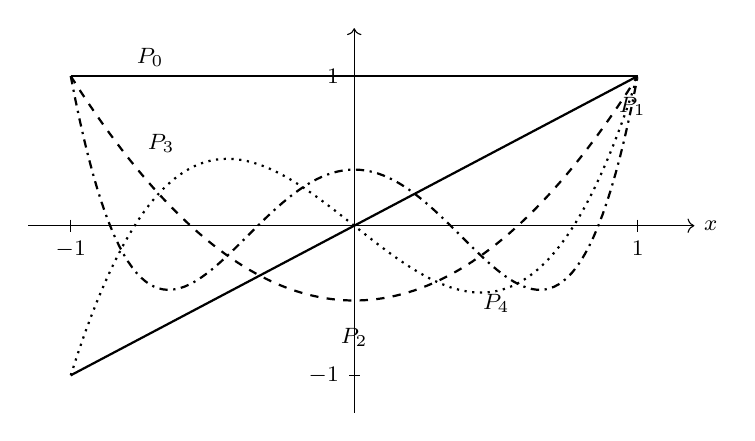
\begin{tikzpicture}[xscale=3.6,yscale=1.9]
\draw[->] (-1.15,0) -- (1.2,0) node[right] {\footnotesize $x$};
\draw[->] (0,-1.25) -- (0,1.32);
\foreach \x in {-1,1} \draw (\x,0.04) -- (\x,-0.04) node[below] {\footnotesize $\x$};
\foreach \y in {-1,1} \draw (0.02,\y) -- (-0.02,\y) node[left] {\footnotesize $\y$};
\draw[thick,domain=-1:1,samples=2]  plot (\x,1);
\node[above] at (-0.72,1.0) {\footnotesize $P_0$};
\draw[thick,domain=-1:1,samples=2]  plot (\x,\x);
\node[right] at (0.90,0.80) {\footnotesize $P_1$};
\draw[thick,dashed,domain=-1:1,samples=90] plot (\x,{1.5*\x*\x-0.5});
\node[below] at (0.0,-0.62) {\footnotesize $P_2$};
\draw[thick,dotted,domain=-1:1,samples=110] plot (\x,{2.5*\x*\x*\x-1.5*\x});
\node[left] at (-0.60,0.55) {\footnotesize $P_3$};
\draw[thick,dash dot,domain=-1:1,samples=130]
  plot (\x,{4.375*\x*\x*\x*\x-3.75*\x*\x+0.375});
\node[right] at (0.42,-0.52) {\footnotesize $P_4$};
\end{tikzpicture}
\caption{The first five Legendre polynomials on $[-1,1]$. Each satisfies
$P_n(1)=1$ and $P_n(-1)=(-1)^n$, and $P_n$ has exactly $n$ zeros in the open
interval --- a property shared by the eigenfunctions of any Sturm--Liouville
problem, and the reason these polynomials interlace as they do.}
\label{fig:legendre}
\end{figure}

Using the Binomial expansion, we can rewrite the expression for the $n^{\text{th}}$ Rodrigues' 
$$(x^2 - 1)^n = \sum_{k = 0}^n \frac{(-1)^k\, n!}{k!\, (n - k)!}\, x^{2(n-k)},$$ so that 
$$P_n(x) = \sum_{k = 0}^{[n/2]} \frac{(-1)^k\, (2n - 2k)!}{2^n\, k!\, (n - k)!\, (n - 2k)!}\, x^{n-2k},$$
where $[n/2]$ denotes the largest integer $\leq \frac{n}{2}$ from Rodrigues' formula, it follows that $P_n(x)$ is a polynomial of degree $n$, and the coefficient of $x^n$ is $$\frac{\binom{2n}{n}}{2^n}$$
We can normalise $P_n(x)$ by multiplying the coefficients by $2^n/\binom{2n}{n}$, so that the coefficient of $x^n$ is 1.

\subsection{Generating Function}
Another definition of Legendre polynomials is obtained by means of the generating function, $$g(x,r) = \frac{1}{(1 - 2rx + r^2)^{1/2}},$$ by expanding it in as a power series for sufficiently small values of $r$. The coefficient of $r^n$ in this expansion turns out to be $P_n(x)$, $\, n = 0, \, 1, \, 2,\, \cdots$ that is
$$g(x,r) = \sum_{n = 0}^{\infty} P_n(x) \, r^n.$$

To show this, consider expanding $(1 - z)^{-1/2}$ in a neighborhood of zero, where 
\begin{align*}
z & = 2rx - r^2,\\
  & = 1 + \frac{1}{2}z + \frac{3}{8}z^2 + \frac{5}{16}z^3 + \, \cdots\cdots\, , \hspace{0.3cm} |z| < 1\\
  & = 1 + \frac{1}{2}(2rx - r^2) + \frac{3}{8}(2rx - r^2)^2  + \frac{5}{16}(2rx - r^2)^3 + \, \cdots\cdots\, \\
  & = 1 + rx + \left(\frac{3}{2}x^2 - \frac{1}{2}\right)r^2 + \left(\frac{5}{2}x^3 - \frac{3}{2}x\right) r^3 + \, \cdots\cdots
\end{align*}
We observe that the coefficient of $1, \, r, \, r^2\,$ and $\, r^3\,$ are exactly, $P_0(x), \, P_1(x),\, P_2(x)$ and $P_3(x)$ respectively.

We generalise thus by the recurrence relation below.

We have $$g(x,r) = \frac{1}{(1 - 2rx + r^2)^{1/2}}.$$
Differentiating this with respect to $r$, we get, from 
$$(1 - 2rx + r^2)^{\frac{1}{2}}\, g(x, r) = 1$$
$$(1 - 2rx + r^2)^{\frac{1}{2}}\, \frac{\partial }{\partial r}g(x, r) + \frac{1}{2}(1 - 2rx + r^2)^{-\frac{1}{2}}\, (-2x + 2r)\, g(x,r) = 0$$
$$(1-2rx + r^2) \frac{\partial}{\partial r}g(x,r) - (x-r)g(x,r) = 0$$
substituting
$$g(x,r) = \sum_{n=0}^{\infty}P_n(x)\, r^n,$$ get
$$(1 - 2rx + r^2) \sum^{\infty}_{n=1}n\, P_n(x)\, r^{n-1}\, -(x-r)\sum_{n=0}^{\infty} P_n(x)\, r^n  = 0.$$
The coefficient of $r^n$ must be zero for each $n$ and for all values of $x$, we thus have
$$(n+1)\, P_{n+1}(x) - (2n +1)xP_n(x) + nP_{n-1}(x) = 0,$$ for $n = 1, \, 2,\, 3,\, \cdots$


This relation connects three successive Legendre polynomials, e.g for $$P_2(x) = \frac{3}{2}x^2 - \frac{1}{2}\, , \hspace{0.5cm} P_3(x) = \frac{5}{2}x^3 - \frac{3}{2}x,$$ then 
$$P_4(x) = \frac{1}{4}\left[7x\, P_3(x) - 3P_2(x)\right] = \frac{35}{8}x^4 - \frac{30}{8}x^2 + \frac{3}{8}.$$
\vspace{6pt}





\begin{exa}
Using $$g(x,r) = \sum_{n=0}^{\infty} P_n(x)\, r^n$$ and $x = 1,\, -1, \, 0,$ show that 
$$P_n(1) = 1, \hspace{0.3cm} P_n(-1) = (-1)^n$$
$$ P_{2n}(0) = \frac{(-1)^n\, \cdot\, 1\, \cdot\, 3\, \cdots\, (2n-1)}{2\, \cdot\, 4\, \cdots \, 2n},$$ 
$P_{2n+1}(0)  = 0.$
\end{exa}


\begin{proof}[Working]
For $x = 1$, we have $$\sum_{n=0}^{\infty} P_n(1)\, r^n = g(1,r) = \frac{1}{(1 - 2r + r^2)^{\frac{1}{2}}}  = \frac{1}{1 - r},$$
geometric i.e $\sum^{\infty}_{n=0} r^n.$


Thus comparing coefficients, get $P_n(1) = 1,$ $\, x = -1$, gives
\begin{align*}
\sum_{n=0}^{\infty} P_n(-1)\, r^n & = g(-1,r)\\
                                  & = \frac{1}{(1 + 2r + r^2)^{\frac{1}{2}}}\\
                                  & = \frac{1}{1 + r}\\
                                  & = \sum^{\infty}_{n=0} (-1)^n\, r^n.
\end{align*}
Thus, $P_n(-1) = (-1)^n.$

$x  = 0$ gives
$$\sum_{n=0}^{\infty} P_n(0)\, r^n = g(0,r) = \frac{1}{(1 + r^2)^{\frac{1}{2}}}$$
Using the binomial  expansion for rational powers
$$(1 + r^2)^{-\frac{1}{2}} = 1 - \frac{1}{2}r^2 + \frac{\left(-\frac{1}{2}\right)\left(-\frac{3}{2}\right)}{2!} r^4 + \frac{\left(-\frac{1}{2}\right)\left(-\frac{3}{2}\right)\left(-\frac{5}{2}\right)}{3!} r^6 + \, \cdots\, + \frac{(-1)(-3)(-5)\, \cdots\, (-(2n-1)}{2^n\, n!} \, + \, \cdots$$
Hence, 
$$P_{2n}(0) = \frac{(-1)^n\, \cdot\, 1\, \cdot\, 3\, \cdot\, 5\, \cdot\, \cdots\, (2n-1)}{2\, \cdot\, 4\, \cdot\, \cdots\, 2n}.$$
Further $P_{2n+1}(0) = 0.$ [coefficient for odd powers is zero]
\end{proof}




\subsubsection{Further Recurrence Relations}
From $$g(x,r) = \frac{1}{(1 - 2rx + r^2)^{\frac{1}{2}}},$$ get $$(1 - 2rx + r^2)^{\frac{1}{2}}\, g(x,r) = 1.$$ Differentiating with respect to $x$, get 
$$(1 -  2rx + r^2)\frac{\partial}{\partial x}g(x,r) - r\, g(x,r) = 0.$$
But $$g(x,r) = \sum_{n=0}^{\infty} P_n(x)\, r^n,$$ so replacing, get $$(1 - 2rx + r^2)\sum_{n=0}^{\infty} P_n'(x) r^n - \sum_{n=0}^{\infty} P_n(x)\, r^{n+1} = 0$$ which implies 
\begin{equation}
P_{n+1}'(x) - 2xP_n'(x) + P_{n-1}'(x) - P_n(x) = 0, \hspace{0.5cm} n=1,\, 2,\, 3,\, \cdots
\end{equation}



Now using $$(n+1)P_{n+1}(x) - (2n+1)xP_n(x) + n P_{n-1}(x) = 0$$ derived in 4.2.1, and differentiating with respect to $x$, get \begin{equation}
(n+1)\, P_{n+1}'(x) - (2n+1) \, P_n(x) - (2n + 1)\, x\, P'_n(x) + nP'_{n-1}(x) =0.
\end{equation}

Eliminating $P'_{n-1}(x)$ from (4.1) and (4.2), get multiplying equation (4.1) by $n$ we obtain 
$$n P_{n+1}'(x)  - 2x nP'_n(x) + nP'_{n-1}(x) -n P_n(x) =  0$$

$$(n+1) P'_{n+1}(x) - (2n+1)P_n(x) - (2n+1)xP_n'(x) + n P'_{n-1}(x) = 0$$
subtracting equation (4.1) from (4.2)
$$P'_{n+1}(x) - (n+1)P_n(x) - xP'_n(x) = 0$$ or
\begin{equation}
P'_{n+1}(x) - xP_n'(x)  = (n+1)P_n(x)
\end{equation}

Similarly, eliminating $P'_{n+1}(x)$ from (4.1) and (4.2), we get
\begin{equation}
xP'_n(x) - P'_{n-1} (x) = nP_n(x)
\end{equation}

Adding (4.3) and (4.4), get 
$$P'_{n+1}(x) - P'_{n-1}(x) = (2n+1) P_n(x), \, \hspace{0.5cm} n = 1, \, 2,\, 3, \, \cdots$$ 
Replacing $n$ by $n-1$ in (4.3), get
\begin{equation}
P'_n(x) - xP'_{n-1}(x)  = nP_{n-1}(x).
\end{equation}


Then we eliminate $P'_{n-1}(x)$ from (4.4) and (4.5), get (by multiplying equation 4.4 by $x$)
$$x^2P'_n(x) - xP'_{n-1}(x) = xnP_n(x)$$
$$P'_n(x) - x P'_{n-1}(x) = n P_{n-1}(x)$$
implies that 
\begin{equation}
(x^2-1)P_n'(x) = nP_{n-1}(x) - n xP_n(x).
\end{equation}

Differentiating (4.6) with respect to $x$ and then using (4.4) to eliminate $P'_{n-1}(x)$, we get
$$\left[(1-x^2)P_n'(x)\right]' + n(n+1) P_n(x) = 0$$
which shows that $U=P_n(x)$ is a particular integral of the second order differential equations.

$$\left[(1-x^2)U'\right]' + n(n+1) U = 0.$$


\subsection{Orthogonality of Legendre Polynomials}
Orthogonality of Legendre polynomials on the interval $[-1,1]$ follows from the Legendre differential equations 
$$\left[(1-x^2)\, P'_n(x) \right]' + n(n+1)\, P_n(x) = 0\hspace{0.5cm} n = 0,\, 1, \, 2,\, \cdots$$ 
We have
\begin{equation}
\left[(1 - x^2)\, P_n'(x)\right]'\, P_m(x) + n(n+1)\, P_n(x)\, P_m(x) = 0
\end{equation}
and 
\begin{equation}
\left[(1-x^2)\, P'_m(x)\right]'\, P_n(x) + m(m+1)\, P_m(x)\, P_n(x) = 0
\end{equation}
subtracting (4.7) from (4.8), get
$$\left\{(1-x^2)\, \left[P'_m(x)\, P_n(x) - P_n'(x)\, P_m(x)\right]\right\}' + (m-n)(m+n-1)P_m(x)P_n(x) = 0.$$
Integrating this last equation over $[-1,1]$ and noting that the first integral vanishes, get
$$(m-n)(m+n+1)\int_{-1}^1P_m(x)\, P_n(x)\, dx = 0$$
i.e 
$$\int_{-1}^1P_m(x)\, P_n(x)\, dx = 0 \hspace{0.7cm} \text{when}\,\,\, m\neq n.$$

Further, it can be shown that
$$\int_{-1}^1P_n^2(x)\, dx = \frac{2}{2n + 1}\, , \hspace{0.6cm} n = 0, \, 1, \, 2, \, \cdots$$


To show this, one uses a recurrence relation
\begin{equation}
(n+1)P_{n+1}(x) - (2n+1)xP_n(x) + nP_{n-1}(x) = 0, \hspace{0.5cm} n = 1, \, 2,\, \cdots 
\end{equation}
Reduce $n$ by $n-1$ in (4.9) and multiply the result by $(2n+1)P_n$.

Then from this equation we subtract (4.9) multiplied by $(2n-1)P_{n-1}(x)$.

Finally integrate the result over $[-1,1]$, noting orthogonality to get 
\begin{align*}
\int_{-1}^1P_n^2(x)\, dx & = \frac{2n - 1}{2n+1}\int_{-1}^1P^2_n(x)\, dx\\
                         & = \frac{3}{2n+1}\int_{-1}^1P^2_1(x)\, dx \hspace{0.6cm} \text{letting} \,\,\, n-1 = 1 \implies n  = 2\\
                         & =\frac{2}{2n+1}.
\end{align*}




\subsection{Expansion of a Function using Legendre}
\vspace{-5mm}
Suppose that $f(x)$ is a function defined on $[-1,1]$ such that
$$\int_{-1}^1f(x)\, P_n(x)\, dx\hspace{0.6cm} \text{exists for }\,\, \, \, n = 0,\, 1,\, 2, \, \cdots$$

Consider the series 
\begin{equation}
f(x) = \sum_{i=0}^{\infty} a_iP_i(x).
\end{equation}
Multiplying both sides of (4.10) by $P_n(x)$ and integrating over $[-1,1]$, get
$$\int_{-1}^1f(x)\, P_n(x)\, dx = \int_{-1}^1a_n\, P^2_n(x)\, dx\, , \hspace{0.3cm} n = 0,\, 1,\, 2, \, \cdots$$
Thus 
\begin{align*}
a_n  & = \left[\int_{-1}^1P^2_n(x)\, dx \right]^{-1}\, \int_{-1}^1f(x)\, P_n(x)\, dx\\\\
     & = \frac{2n + 1}{2}\int^1_{-1} f(x) \, P_n(x)\, dx.
\end{align*}


Recall Fourier series 
$$f(x) = \sum_{n=0}^{\infty}\left[a_n\cos nx + b_n \sin nx\right].$$ 
\vspace{0.5cm}



\begin{exa}
Suppose $$f(x) = \begin{cases}
                   0, & -1\leq x \leq \alpha\\
                   1, & \alpha x \leq 1.\\
                 \end{cases}$$
Expand $f(x)$ in series of Legendre polynomials.                 
\end{exa}


\begin{proof}[Working]
Using the recurrence relation
$$P'_{n+1}(x) - P'_{n-1}(x) = (2n + 1)P_n(x), \hspace{0.4cm} n = 1, \, 2, \, \cdots$$
we have
\begin{align*}
a_n & = \frac{2n + 1}{n} \int_{\alpha}^1P_n(x) \, dx\\
    & = \frac{1}{2}\int_{\alpha}^1\left[P'_{n+1}(x) - P_{n-1}'(x)\right]\, dx\\
    & = \frac{1}{2}\left[P_{n+1}(x) - P_{n-1}(x)\right]'_{x=\alpha}\\
    & = -\frac{1}{2}\left[P_{n+1}(\alpha) - P_{n-1}(\alpha)\right]\, , \hspace{0.5cm} \text{since}\,\,\, P_n(1) = 1.
\end{align*}
Hence
$$f(x)  = \sum_{i=0}^{\infty} a_i \, P_i(x) = \frac{1}{2}(1 - \alpha)-\frac{1}{2}\sum_{i=1}^{\infty} \left[P_{i+1}(\alpha) - P_{i-1}(\alpha)\right]\, P_i(x).$$
\end{proof}
\vspace{0.5mm}

\begin{exe}
\vspace{-6pt}
\begin{enumerate}
\item Show that the sequence
$$\left\{\frac{1}{\sqrt{2}}, \, \sin x, \, \cos x, \, \sin 2x, \, \cos 2x, \, \cdots\, , \, \sin nx, \, \cos nx\right\}$$ is orthogonal with respect to $w(x) = \frac{1}{\pi}$ over $[-\pi, \pi]$. \\
\textit{Hint:} $$ \int_{-\pi}^{\pi} \frac{1}{\sqrt{2}}\, \sin nx\, dx\, , \hspace{0.5cm} \int_{-\pi}^{\pi} \frac{1}{\sqrt{2}}\, \cos nx\, dx\, , \hspace{0.5cm} \int_{-\pi}^{\pi} \sin nx\, \cos nx\, dx$$


\item If $f(x) = |x|, \,\, -1 \leq x \leq 1$, show that 
$$f(x) = \sum_{n=0}^{\infty} a_n\, P_n(x) = \sum_{n=0}^{\infty} \frac{(-1)^{n+1}\,(4n+1)\, (2n-2)!}{2^{2n}\, (n+1)!\, (n-1)!}\, P_{2n}(x).$$
\textit{Hint:} At some stage $$a_n = 2\int_0^1 x\, P_n(x)\, dx,$$ use recurrence relation when $n=$ odd $\implies n$ is will be zero.


\item Show that $$\int_{-1}^1x\, P_n(x)\, P_{n-1}(x)\, dx = \frac{2n}{4n^2 - 1}.$$

\item If $$\begin{cases}
            \frac{1}{2}\, , & 0 < x < 1\\
            -\frac{1}{2}\, , & -1 < x < 0\\
           \end{cases}$$ expand $f(x)$ in the form $\sum_{n=0}^{\infty}a_n\, P_n(x)$.
\end{enumerate}
\end{exe}
\vspace{5mm}


















% Jacobi Polynomials
\section{Jacobi Polynomials}
\vspace*{-5mm}
Jacobi polynomials generalize the Legendre polynomials.

\begin{defn}
The Jacobi polynomials are defined by the Rodrigues' formula $$P_n^{\alpha,\beta}(x) = \frac{(-1)^n}{2^n\, n!}\, (1 - x)^{-\alpha}\, (1 + x)^{-\beta}\, \frac{d^n}{dx^n}\left[(1 - x)^{\alpha + n}(1 + x)^{\beta + n}\right]$$ 
$n = 0, \, 1, \, 2, \, \, \cdots\cdots$

These polynomials are orthogonal on $[-1,1]$ with weight function.
$$w(x) = (1 - x)^{\alpha}\, (1 + x)^{\beta}\hspace{0.4cm}\text{for}\hspace{0.4cm} \alpha > -1, \hspace{0.2cm} \beta > -1.$$
The restrictions on $\alpha$ and $\beta$ ensure that $w(x)$ is integrable on $[-1,1]$. When $\alpha = \beta = 0$, we get the Legendre polynomials.
\end{defn}



\begin{thm}
The Jacobi polynomials i.e $$P_n^{(\alpha,\beta)} (x)  = \sum_{k = 0}^n \frac{\Gamma(\alpha + n + 1)\, \Gamma(\beta + n + 1)\, \left(\frac{x - 1}{2}\right)^k\, \left(\frac{x + 1}{2}\right)^{n - k}}{\Gamma (\alpha + k + 1)\, \Gamma (\beta + n - k + 1)\, k!\, (n-k)!}.$$
\end{thm}

\begin{proof}
We use Leibniz's formula for derivative of a product, to get
\begin{align*}
\frac{d^n}{dx^n}\left[(1 - x)^{\alpha + n}\, (1 + x)^{\beta + n}\right]  = & \sum^n_{k=0} \frac{n!}{k!\, (n-k)!}\left\{\frac{d^k}{dx^k}(1  + x)^{\beta + n}\right\}\left\{\frac{d^{n-k}}{dx^{n-k}}(1 - x)^{\alpha + n}\right\}\\
 = & \sum^n_{k=0}\frac{n!}{k!\, (n-k)!}\, (\beta + n)(\beta + n -1)\, \cdots\, (\beta + n - k + 1)(1+x)^{\beta + n - k}\\
   & \times (-1)^{n-k}\, (\alpha + n)(\alpha + n - 1)\, \cdots\, (\alpha + n - n + k + 1)(1 - x)^{\alpha + k}\\
 = & \sum^n_{k = 0} \frac{n!\, (-1)^{n-k}}{k!\, (n-k)!}\frac{\Gamma(\beta + n + 1)\, \Gamma(\alpha + n + 1)}{\Gamma(\beta + n - k + 1)\, \Gamma(\alpha + k + 1)}\, (1 + x)^{\beta + n - k}\, (1 - x)^{\alpha + k}
\end{align*}

where we have used $\Gamma(x + 1) = x\Gamma(x)$. Replacing in Rogrigues formula get
\begin{align*}
P_n^{(\alpha,\beta)}(x) & = \frac{(-1)^n}{2^n\, n!}\, (1 - x)^{-\alpha}\, (1 + x)^{-\beta}\, \frac{d^n}{dx^n}\left[(1 + x)^{\beta + n}(1 - x)^{\alpha + n}\right]\\
& = \sum^n_{k=0}\frac{\Gamma(\alpha + n  + 1)\, \Gamma(\beta + n + 1)\, \left(\frac{x - 1}{2}\right)^k\, \left(\frac{x + 1}{2}\right)^{n-k}}{\Gamma(\alpha + k + 1)\, \Gamma (\beta + n-k +1)\, k!\, (n-k)!}.
\end{align*}
\end{proof}





\begin{exe}\textbf{}
\begin{enumerate}
\item[(a).] Show that $$P_n^{(\alpha,\beta)}(-x) = (-1)^n\, P_n^{(\alpha,\beta)}(x).$$
\item[(b).] Show that $$P^{(\alpha,\beta)}_n(1) = \frac{\Gamma\left(\alpha + n + 1\right)}{\Gamma(\alpha + 1)\, n!}.$$
\end{enumerate}
\end{exe}



\section{Chebyshev Polynomials of the First Kind}
\begin{defn}
Chebyshev's polynomials of the first kind denoted by $T_n(x)$, are defined by $$T_n(x) = \cos \left(n\, \cos^{-1}x\right),$$ $n= 0,\, 1,\, 2,\, \cdots$ and $0\leq \cos^{-1}(x) \leq \pi$.
\end{defn}



We immediately set that $\, -1 \leq T_n(x) \leq 1$.


\begin{thm}
$$T_n(x) = \frac{1}{2}\left[\left\{x + i\sqrt{1 - x^2}\right\}^n + \left\{x - i\sqrt{1 - x^2}\right\}^n\right]$$
\end{thm}

\begin{proof}
Let $x = \cos \theta$. Then
\begin{align*}
T_n(x)  = \cos \left(n\, \cos^{-1}x\right) & = \cos n\theta\\
                                           & = \frac{1}{2}\left[e^{in\theta} + e^{-in\theta}\right]\\
                                           & = \frac{1}{2}\left[\left(e^{i\theta}\right)^n + \left(e^{-i\theta}\right)^n\right]\\
                                           & = \frac{1}{2}\left[\left\{\cos \theta + i\sin \theta\right\}^n + \left\{\cos \theta - i\sin \theta\right\}^n\right]\\
                                           & = \frac{1}{2}\left[\left\{x + i \sqrt{1 - x^2}\right\}^n + \left\{x - i\sqrt{1 - x^2}\right\}^n \right].
\end{align*}
\end{proof}






\begin{thm}
$$T_n(x) = \sum_{k =0 }^{\left[\frac{n}{2}\right]}\frac{(-1)^n\, n!}{(2k)!\, (n-2k)!}\, (1 - x^2)^k\, x^{n-2k}.$$
\end{thm}

\begin{proof}
From 4.4.2
\begin{align*}
T_n(x) & = \frac{1}{2}\left[\left\{x + i\sqrt{1 - x^2}\right\}^n + \left\{x - i\sqrt{1 - x^2}\right\}^n\right]\\
       & = \frac{1}{2}\left[\sum^{n}_{k = 0} \binom{n}{k}\, x^{n-k}\, \left\{i\sqrt{1 - x^2}\right\}^k \, + \, \sum_{k=0}^n\binom{n}{k}\, x^{n-k}\, \left\{-i\sqrt{1 - x^2}\right\}^k\right]\\
       & = \frac{1}{2}\sum^n_{k=0}\binom{n}{k}\, x^{n-k}\, (1 - x^2)^{k/2}\, \left[1 + (-1)^k\right] \, i^k\\
       & = \frac{1}{2}\sum^n_{k=0}\binom{n}{k}x^{n-k}(1-x^2)^{k/2}\left[1 + (-1)^k\right]\, i^k.
\end{align*}
Now when $k = $ odd then $1 + (-1)^k  = 0$, and when $k = $ even then $1 + (-1)^k = 2$.  Hence, 
$$T_n(x) = \frac{1}{2}\sum_{k = \, \text{even}\, \leq n} \binom{n}{k} x^{n-k}(1 - x^2)^{k/2}\, i^k \cdot 2$$
But when $k = $ even, we have $k = 2s$ for some integers $s$. $k \leq n$ means that $s \leq \frac{n}{2}$. Since $s$ is an integer, $s \leq \frac{n}{2}$ means $s \leq \left[\frac{n}{2}\right]$. Thus 
\begin{align*}
T_n(x) & = \sum^{\left[\frac{n}{2}\right]}_{s = 0} \binom{n}{2s} x^{n-2s} (1 - x^2)^{s}\, i^{2s}\\
       & = \sum^{\left[\frac{n}{2}\right]}_{s =0} \frac{n!}{(2s)!\, (n-2s)!}x^{n-2s}(1 - x^2)^s(-1)^s.
\end{align*}
\end{proof}


Using theorem 4.4.3 we have 
$$ T_0(x) = 1, \hspace{0.5cm} T_1(x) = x, \hspace{0.5cm} T_2(x) = 2x^2 - 1, \hspace{0.5cm} T_3(x) = 4x^3 - 3x, \hspace{0.5cm} T_4(x) = 8x^4 - 8x^2 + 1,$$  $$ T_5(x) = 16x^5 - 20x^3 + 5x.$$


\begin{thm}\textbf{}
\vspace{-4mm}
\begin{multicols}{3}
\begin{enumerate}
\item[(a).] $T_n(1) = 1$
\item[(b).] $T_n(-1) = (-1)^n$
\item[(c).] $T_n(-x) = (-1)^n\, T_n(x)$
\item[(d).] $T_{2n}(0) = (-1)^n$
\item[(e).] $ T_{2n+1}(0) = 0.$
\end{enumerate}
\end{multicols}
\end{thm}

\begin{proof}
We use the definitions of $T_n(x)$
\vspace{-3mm}
\begin{enumerate}
\item[(a).] $T_n(1) = \cos \left(n\, \cos^{-1} 1\right) = \cos (n\, (0)) = 1.$

\item[(b).] $T_n(-1) = \cos\left(n\, \cos^{-1}\, (-1)\right) = \cos (n\pi) = (-1)^n.$

\item[(c).] $T_n(-x)$
\begin{align*}
T_n(-x) & = \frac{1}{2}\left[\left\{-x + i\sqrt{1 - x^2}\right\}^n + \left\{-x - i\sqrt{1 - x^2}\right\}^n\right]\\
        & = \frac{1}{2}\left[(-1)^n\left\{x - i\sqrt{1 - x^2}\right\}^n + (-1)^n\left\{x + i\sqrt{1 - x^2}\right\}^n\right]\\
        & = (-1)^n\, T_n(x).
\end{align*}

\item[(d).] $T_{2n}(0) = \frac{1}{2}\left[(i)^{2n}  + (-i)^{2n}\right] = \frac{1}{2}\left[(-1)^n + (-1)^n\right] = (-1)^n\,$ by using 4.4.2

\item[(e).] $T_{n+1}(0) = \frac{1}{2}\left[(i)^{2n+1}  + (-i)^{2n+1}\right] = \frac{1}{2}\left[(-1)^n\, i - (-1)^n\, i\right] = 0.$
\end{enumerate}
\end{proof}


\begin{exe}
Show that $\, T_n(x)\,$ is a solution of Chebyshev's equation $$(1 - x^2)\frac{d^2y}{dx^2} - x\frac{dy}{dx} + n^2 y = 0.$$ 
\textit{Hint:} let $y = T_n(x)$.
\end{exe}


\begin{thm}[\textit{Orthogonality property.}]
$$\int_{-1}^1\frac{T_m(x)\, T_n(x)}{\sqrt{1 - x^2}}\, dx = \begin{cases}
                                                            0, & m\neq n\\
                                                            \frac{\pi}{2}, & m = n \neq 0\\
                                                            \pi, & m = n = 0.
                                                           \end{cases}$$
\end{thm}

\begin{proof}
Let $\, x = \cos \theta, \hspace{0.5cm} dx  = -\sin \theta\, d\theta\,\,$ and $\sqrt{1 - x^2} = \sin \theta$, so 
\begin{align*}
\int_{-1}^1\frac{T_m(x)\, T_n(x)}{\sqrt{1 - x^2}}\, dx & = \int_{\pi}^0\frac{T_m(\cos \theta)\, T_n(\cos\theta)\, (-\sin\theta\, d\theta)}{\sin\theta}\\
& = \int^{\pi}_0\cos n\theta\, \cos m\theta \, d\theta,
\end{align*}
\begin{align*}
T_n(\cos \theta)   = \cos\left(n\, \cos^{-1}(\cos \theta)\right)
                 & = \cos n\theta\\
                 & = \frac{1}{2}\int_0^{\pi}\left[\cos (m+n)\theta + \cos (n-m)\theta\right]\, d\theta\\
                 & = \frac{1}{2}\left[\frac{\sin (m+n)\theta}{m+n} + \frac{\sin (n-m)\theta}{n-m}\right]^{\pi}_0\\
                 & = 0, \hspace{0.6cm} m\neq n.
\end{align*}

If $m = n \neq 0$, we have 
\begin{align*}
\int_{-1}^1T_n(x)\, T_n(x)\, dx & = \int_0^{\pi}\cos^2 n\theta \, d\theta\\
                                & = \int_0^{\pi}\frac{1}{2}(1 + \cos 2n\theta)\, d\theta\\
                                & = \frac{\pi}{2}.
\end{align*}
If $m = n = 0,$
$$\int^1_{-1}\frac{T_0(x)\, T_0(x)}{\sqrt{1 - x^2}}\, dx = \int^{\pi}_0 d\theta = \pi.$$
\end{proof}






\begin{thm}[\textit{Recurrence Relations}]\textbf{}
\vspace{-4mm}
\begin{enumerate}
\item[(a).] $T_{n+1}(x) - 2xT_n(x) + T_{n-1}(x) = 0$
\item[(b).] $(1 - x^2)T_n'(x) = -nxT_n(x) + nT_{n-1}(x).$\\
\end{enumerate}
\end{thm}


Notice that $$x = \cos \theta\, \implies\, \begin{cases}
                                            T_{n+1}(x) & = \cos (n+1)\theta\\
                                            T_{n-1}(x) & = \cos (n-1)\theta.
                                           \end{cases}$$








\begin{exe}\textbf{}
\vspace{-4mm}
\begin{enumerate}
\item[(a).]  Show that $$\, T_{m+n}(x) + T_{n-m}(x)  = 2\, T_m(x)\, T_n(x).$$

\item[(b).] Show that $$2\left\{T_n(x)\right\}^2 = 1 + T_{2n}(x).$$

\item[(c).] Show that $$\left\{T_n(x)\right\}^2 - T_{n+1}(x)\, T_{n-1}(x) = 1 - x^2.$$

\item[(d).] Show that $$T_m(T_n(x)) = T_n(T_m(x)) = T_{m+n}(x).$$

\item[(e).] Let $\{T_n(x)\}^{\infty}_{n=0}$ be a sequence of the Chebyshev polynomials of the first kind. Let $$\xi_i = \cos\left[(2i - 1)\frac{\pi}{2n}\right]\, , \hspace{0.4cm} i = 1,\, 2,\, \cdots\, n.$$
   \begin{enumerate}
   \item[(i).] Verify that $\xi_1, \, \xi_2, \, \cdots\, , \, \xi_n$ are zeros of $T_n(x)$ that is $\,T_n(\xi_i) = 0\,$ for $i = 1, \, 2, \, \cdots\, , \, n$.
   
   \item[(ii).] Show that $\xi_1, \, \xi_2, \, \cdots \, , \, \xi_n$ are simple zeros of $\,T_n(x)$. i.e $\,T_n'(\xi_i) \neq
    0, \hspace{0.3cm} i = 1, \, 2,\, \cdots\, , \, n.$
   \end{enumerate}
\end{enumerate}

\end{exe}


%%%%%%%%%%%%%%%%%%%%%%%%%%%% Chebyshev polynomials of the second kind
\section{Chebyshev Polynomials of the Second Kind}
\begin{defn}
The Chebyshev polynomials of the second kind are defined in terms of Chebyshev polynomials of the first kind as follows. Differentiating $$T_n(x) = \cos n\theta$$ with respect to $\, x  = \cos \theta$, get
$$\frac{d}{dx} T_n(x)  = -n\, \sin \theta\, \frac{d\theta}{dx} = \frac{n\, \sin n\theta}{\sin \theta}$$
we then define Chebyshev polynomials of the second kind by 
$$U_n(x) = \frac{1}{n + 1}\, \frac{d}{dx}T_{n+1}(x) = \frac{\sin[(n + 1)\theta]}{\sin \theta}\, , \hspace{0.3cm} n = 0, \, 1, \, 2, \, \cdots\cdots$$
We observe that in other context Chebyshev polynomials of the second kind have been defined by 
$$U_n(x) = \sin\left(n\, \cos^{-1}(x)\right) = \sin n\theta, \, \hspace{0.3cm}\text{where}\hspace{0.3cm} x = \cos \theta.$$
\end{defn}









\begin{thm}[Recurrence Relation]\textbf{}
\vspace*{-6mm}
\begin{enumerate}
\item[(a).] $U_n(x) = x U_{n-1}(x) + T_n(x), \hspace{0.4cm} n = 1, \, 2, \, \cdots\cdots$
\item[(b).] $U_n(x) = 2x U_{n - 1}(x) - U_{n-2}(x), \hspace{0.4cm} n = 2, \, 3, \cdots\cdots$
\item[(c).] $(1 - x^2)U_n'(x) = nx U_n(x) + nU_{n-1}(x).$
\end{enumerate}
\end{thm}






\begin{proof}
\begin{enumerate}
\item[(a).] 
\begin{align*}
U_n(x) & = \frac{\sin [(n + 1)\theta]}{\sin \theta}\\
       & = \frac{\sin n\theta \cos \theta + \sin \theta \cos n\theta}{\sin \theta}
         = \cos \theta\left(\frac{\sin n\theta}{\sin \theta}\right) + \cos n\theta\\
       & = xU_{n-1}(x) + T_n(x).
\end{align*}

\item[(b).] Use the identity
$$\sin[(n+1)\theta] + \sin[(n - 1)\theta] = 2\sin n\theta \sin \theta.$$

\item[(c).] Exercise
\end{enumerate}
\end{proof}




\begin{thm}[Orthogonality]
$$\int_{-1}^1U_n(x)\, U_m(x)\, (1 - x^2)^{\frac{1}{2}}\, dx = \begin{cases}
                                                               0, & m\neq n\\
                                                               \frac{\pi}{2}, & m=n\neq 0\\
                                                               0, & m = n= 0\\
                                                              \end{cases}$$
\end{thm}




\begin{proof}
Let \, \, $x = \cos \theta, \hspace{0.3cm} dx = -\sin \theta\, d\theta.$ Then 
$$\int_{-1}^1U_n(x)\, U_m(x)\, (1 - x^2)^{\frac{1}{2}}\, dx = \int_0^{\pi}\sin[(n+1)\theta]\,\sin[(m+1)\theta]\, d\theta = 0, \hspace{0.3cm} m\neq n.$$
\end{proof}



\begin{exe}
Find the values of 
\begin{multicols}{4}
\begin{enumerate}
\item[(a).] $U_n(1)$
\item[(b).] $U_n(-1)$
\item[(c).] $U_{2n}(0)$
\item[(d).] $U_{2n + 1}(0).$
\end{enumerate}
\end{multicols}
\end{exe}


Show that $U_n(x)$ is the solution of the Chebyshev equation 
$$(1 - x^2)\, \frac{d^2y}{dx^2} - x\, \frac{dy}{dx} + n^2 y = 0.$$



%%%%%%%%%%%%% Hermite Polynomials
\section{Hermite Polynomials}
\begin{defn}[Hermite Polynomial]
Hermite polynomials denoted by $H_n(x)$, are defined by the Rodrigues formula of the form 
$$H_n(x) = (-1)^n\, e^{\frac{x^2}{2}}\, \frac{d^n}{dx^n}\left[e^{-\frac{x^2}{2}}\right]\, , \hspace{0.3cm} n = 0, \, 1, \, 2, \, \cdots\cdots$$
\end{defn}



\begin{thm}[Recurrence Relation]
$$H_{n+1}(x) = x\, H_n(x) - H_n'(x)\, , \hspace{0.4cm} n =0, \, 1,\, 2.$$
\end{thm}


\begin{proof}
From the definition of $H_n(x)$, we have
\begin{equation}
\frac{d^n}{dx^n}\left[e^{-\frac{x^2}{2}}\right] = (-1)^n\, e^{-\frac{x^2}{2}}\, H_n(x)
\end{equation}
Differentiating through (4.1), we get
\begin{equation}
\frac{d^{n+1}}{dx^{n+1}}\left[e^{-\frac{x^2}{2}}\right] = (-1)^n\left[-xe^{-\frac{x^2}{2}}\, H_n(x) + e^{-\frac{x^2}{2}}\, H_n'(x)\right]
\end{equation}
Again using the definition, get
\begin{equation}
\frac{d^{n+1}}{dx^{n+1}}\left[e^{-\frac{x^2}{2}}\right] = (-1)^{n+1}\, e^{-\frac{x^2}{2}}\, H_{n+1}(x)
\end{equation}
from (4.2) and (4.3) get
$$H_{n+1}(x) = x\, H_n(x) - H_n'(x)\, , \hspace{0.3cm} n = 0, \, 1, 2, \cdots\cdots$$
\end{proof}


\textit{Remark.}\\
Since $H_0(x) = 1$, it follows by induction, using the above relation that $H_n(x)$ is a polynomial of degree $n$ with leading coefficient 1.



\begin{thm}
$$\exp\left(tx - \frac{t^2}{2}\right) = \sum^{\infty}_{n = 0} \frac{t^n}{n!}\, H_n(x).$$
\end{thm}

\begin{proof}
If $w(x) = e^{-\frac{x^2}{2}}$, then 
\begin{equation}
w(x - t) = \exp\left(-\frac{x^2}{2} + tx - \frac{t^2}{2}\right) = e^{-\frac{x^2}{2}}\cdot e^{tx - \frac{t^2}{2}} = w(x)\, \exp\left(tx - \frac{t^2}{2}\right).
\end{equation}
Applying Taylor expansion above we get 
\begin{equation}
w(x -t) = \sum^{\infty}_{n = 0} \frac{(-1)^n}{n!}\, t^n\, \dfrac{d^n}{dx^n}[w(x)] = \sum_{n = 0}^{\infty} \frac{t^n}{n!}\, H_n(x)\, w(x),
\end{equation}
since 
$$H_n(x) = (-1)^n\, e^{\frac{x^2}{2}}\, \frac{d^n}{dx^n}[w(x)].$$
Then using (4.4) and (4.5), get
$$\exp\left(tx - \frac{t^2}{2}\right) = \sum_{n = 0}^{\infty} \frac{t^n}{n!}\, H_n(x).$$
\end{proof}




\begin{thm}
$$H_n(x) = \sum_{r = 0}^{\left[\frac{n}{2}\right]}\frac{n!\, (-1)^r\, x^{n - 2r}}{2^r\, (n - 2r)!\, r!}$$
\end{thm}

\begin{proof}
From theorem 4.6.3,
\begin{align*}
\sum^{\infty}_{n = 0} \frac{t^n}{n!}\, H_n(x) & = \exp\left(tx - \frac{t^2}{2}\right)\\
 & = e^{tx}\, \cdot\, e^{-\frac{t^2}{2}}\\
 & = \sum_{k= 0}^{\infty} \frac{(tx)^k}{k!}\,\cdot\, \sum_{r = 0}^{\infty} \frac{\left(\frac{-t^2}{2}\right)^r}{r!}\, , \hspace{0.4cm} \text{Maclaurin expansion}\\
 &  = \sum_{k,r = 0}^{\infty}\frac{(-1)^r\, x^k\, t^{k + 2r}}{2^r\, k!\, r!}
\end{align*}
for a fixed value of $r$, we get $t^n$ by setting $k + 2r = n$, so that $k = n - 2r$. So for this value of $r$, the coefficient of $t^n$ is given by $$ \frac{(-1)^r\, x^{n-2r}}{2^r\, (n-2r)!\, r!}.$$ 
Then the total coefficient of $t^n$ is obtained by summing over all allowed values of $r$ since $k = n-2r$, we have $n -2r \geq 0$, or $r \leq \frac{n}{2}$. If $n = $ even, $r$ goes from 0 to $\frac{n}{2}$. If $n = $ odd, $r$ goes from 0 to $\frac{n-1}{2}$.\\
That is in all cases $r$ goes from o to $\left[\frac{n}{2}\right].$ Thus
$$\sum_{r=0}^{\left[\frac{n}{2}\right]}\frac{(-1)^r\, x^{n - 2r}}{2^r\, (n - 2r)!\, r!} = \frac{1}{n!}\, H_n(x)$$
implies $$H_n(x) = \sum_{r=0}^{\left[\frac{n}{2}\right]}\frac{(-1)^r\, x^{n - 2r}}{2^r\, (n - 2r)!\, r!}.$$
\end{proof}


\textit{Remark.}\\
$H_0(x) = 1,$ \hspace{0.3cm} $H_1(x) = x $, \hspace{0.3cm} $H_2(x) = x^2 - 1$, \hspace{0.3cm} $H_3(x) = x^3 - 3x$, \hspace{0.3cm} $H_4(x) = x^4 - 6x^2 + 3$, \hspace{0.3cm} $H_5(x) = x^5 - 10x^3 + 15x$, \hspace{0.3cm} $H_6(x) = x^6 - 15x^4 + 45x^2 - 15$.




\begin{thm}[Recurrence Relation]\textbf{}
\vspace*{-6mm}
\begin{enumerate}
\item[(a).] $H_n'(x) = n\, H_{n-1}(x)$\, , \hspace{0.3cm} $n\geq 1;$ \hspace{0.3cm} $H_0'(x) = 0.$
\item[(b).] $H_{n+1}(x) = x\, H_n(x) - n\, H_{n-1}(x)\, , \hspace{0.3cm} n\geq 1$.  $H_1(x) = x\, H_0(x)$, with $H_0(x) = 1$ and $H_1(x) = x$.
\end{enumerate}
\end{thm}

\begin{proof}
\begin{enumerate}
\item[(a).] Differentiating with respect to $x$, get 
$$\sum_{n = 0}^{\infty} \frac{t^n}{n!}\, H_n'(x) = t\, \exp\left(tx - \frac{t^2}{2}\right) = t \,\sum_{n = 0}^{\infty} \frac{t^n}{n!}\, H_n(x).$$
Let $\,  s  = n + 1$ 
$$ = \sum_{n = 0}^{\infty}\frac{t^{n + 1}}{n!}\, H_n(x) = \sum_{n = 1}^{\infty} \frac{t^n}{(n - 1)!}\, H_{n-1}(x)$$
equating coefficients of $t^n$, for $n = 0$, $H_0'(x) = 0$, and for $n\geq 1$, 
$$\frac{H_n'(x)}{n!} = \frac{H_{n-1}(x)}{(n-1)!}\implies  H_n'(x) = n\, H_{n-1}(x)$$ since $$\frac{n!}{(n-1)!} = \frac{n\, (n-1)!}{(n-1)!}  = n.$$


\item[(b).] Differentiating both sides of $$\exp\left(tx - \frac{t^2}{2}\right) = \sum_{n=0}^{\infty} \frac{t^n}{n!}\, H_n(x)$$ with respect to  $t$, get
$$(x -t)\, \exp\left(tx - \frac{t^2}{2}\right) = \sum_{n=0}^{\infty} \frac{n\ t^{n-1}}{n!}\, H_n(x)$$
observe that for $n =0$, $\frac{n\, t^{n-1}}{n!} = 0$ hence,

$$(x - t) \sum_{n = 0}^{\infty} \frac{t^n}{n!}\, H_n(x) = \sum_{n=1}^{\infty} \frac{t^{n-1}}{(n-1)!}\, H_n(x)$$

$$x\sum_{n=0}^{\infty} \frac{t^n}{n!}\, H_n(x) - \sum_{n=0}^{\infty} \frac{t^{n + 1}}{n!}\, H_n(x) = \sum_{n = 1}^{\infty}\frac{t^{n-1}}{(n-1)!}\, H_n(x)$$

$$x\, \sum_{n=0}^{\infty}\frac{t^n}{n!}\, H_n(x) - \sum_{n=1}^{\infty}\frac{t^{n + 1}}{(n-1)!}\, H_{n-1}(x) = \sum_{n=0}^{\infty} \frac{t^n}{n!}\, H_{n+1}(x)$$
comparing coefficients for $n\geq 1$, get
$$\frac{H_n(x)}{n!} - \frac{H_{n-1}(x)}{(n-1)!} = \frac{H_{n+1}(x)}{n!}\, , $$
multiply by $n!$ then
$$x\, H_n(x) - n\, H_{n-1}(x) = H_{n+1}(x)$$
equating coefficients of $t^0$, get
$$x\, H_0(x) = H_1(x).$$
\end{enumerate}
\end{proof}



\begin{exe}
Using (a) and (b), show that $$H_n''(x) - x\, H_n'(x) + n\, H_n(x)  = 0,$$ so that $H_n(x)$ is a solution of the differential equation $$U'' - x\, U' + n\, U = 0.$$ \textit{Hint:} Eliminate $H_{n-1}(x)$ from (a) and (b).
\end{exe}




\begin{thm}[Orthogonality Properties]
With the weight function $w(x) = e^{-\frac{x^2}{2}}$ over $(-\infty,\infty)$, we have 
$$\int_{-\infty}^{\infty} e^{-\frac{x^2}{2}}\, H_n(x)\, H_m(x)\, dx = n!\, \sqrt{2\pi}\, \cdot\, \delta_{mn},$$ 
where
$$\delta_{mn} = \begin{cases}
                 1, & m = n\\
                 0, & n\neq m.
               \end{cases}$$
\end{thm}

\begin{proof}
Let $$c = \int_{-\infty}^{\infty} e^{-\frac{x^2}{2}}\, H_n(x)\, H_m(x)\, dx.$$
Then by definition of 
$$H_n(x) = (-1)^n\, e^{-\frac{x^2}{2}}\, \frac{d^n}{dx^n}\left(e^{-\frac{x^2}{2}}\right),$$
\begin{align*}
c & = (-1)^n\int_{-\infty}^{\infty}H_m(x)\, \frac{d^n}{dx^n}\left(e^{-\frac{x^2}{2}}\right)\, dx\\
  & = (-1)^n\,H_m(x)\, \frac{d^{n-1}}{dx^{n-1}}\left(e^{-\frac{x^2}{2}}\right)\int^{\infty}_{-\infty}\, \frac{d}{dx}H_m(x)\, \cdot\, \frac{d^{n-1}}{dx^{n-1}}\left(e^{-\frac{x^2}{2}}\right)\, dx
\end{align*}
by integration by parts. $u = H_m(x), \, dv = \frac{d^n}{dx^n}\left(e^{-\frac{x^2}{2}}\right)\, dx$
$$c = (-1)^{n+1}\int_{-\infty}^{\infty}\frac{d}{dx}H_m(x)\, \frac{d^{n-1}}{dx^{n-1}}\left(e^{-x^2}\right)\, dx,$$
Since $$H_m(x)\, \frac{d^{n-1}}{dx^{n-1}}\left(e^{-\frac{x^2}{2}}\right)$$ is a polynomial multiplied by $e^{-\frac{x^2}{2}}$, and so goes to zero as $x\rightarrow \infty$. \\
Integrating by parts $m-1$ more times, get 
\begin{equation}
c = (-1)^{n+m}\int_{-\infty}^{\infty} \frac{d^m}{dx^m}H_m(x)\, \frac{d^{n-m}}{dx^{n-m}}\left(e^{-\frac{x^2}{2}}\right)\, dx 
\end{equation}
Now, since $H_m(x)$ is a polynomial of degree $m$ with leading coefficient 1, 
$$\frac{d^m}{dx^m}H_m(x) = m!,$$ so that
$$c = (-1)^{n+m}\int^{\infty}_{-\infty} \frac{d^{n-m}}{dx^{n-m}}\left(e^{-\frac{x^2}{2}}\right)\, dx = \frac{d^{n-m-1}}{dx^{n-m-1}}\left[e^{-x^2}\right]^{\infty}_{-\infty} = 0,$$
since $n>m$, and so $n-m-1 > 0$.\\
The case $m<n$ is arrived at in the same way, hence, 
$$\int_{-\infty}^{\infty}e^{-\frac{x^2}{2}}\, H_m(x)\, H_n(x)\, dx = 0, \hspace{0.3cm} m\neq n.$$
When $m = n$,
\begin{align*}
c & = \int_{-\infty}^{\infty}\frac{d^n}{dx^n}[H_n(x)]\, e^{-\frac{x^2}{2}}\, dx \hspace{0.4cm} \text{from 4.6}\\
  & = n! \int_{-\infty}^{\infty} e^{-\frac{x^2}{2}}\, dx,\,\, \text{since}\, \, H_n(x)\,\, \text{is of degree}\,\, n\,\, \text{with leading coefficient 1}\\
  & = 2n! \int_0^{\infty} e^{-\frac{x^2}{2}}\, dx\\
  & = 2n!\left(\frac{\sqrt{2}}{2}\,\sqrt{\pi}\right)\\
  & = n!\, \sqrt{2\pi}, \hspace{0.3cm} \text{since}\hspace{0.3cm} 2\int_0^{\infty} e^{-t^2}\, dt = \sqrt{\pi},\, \, t^2 = \frac{x^2}{2}.
\end{align*} 
\end{proof}




\subsubsection{Series Expansions in Terms of Hermite Polynomials}
Hermite polynomials can be used to express a function $f(x)$ in the form
$$f(x) = \sum_{n=0}^{\infty}c_n\, H_n(x)$$ where 
$$c_n = \frac{1}{n!\, \sqrt{2\pi}}\int_{-\infty}^{\infty} e^{-\frac{x^2}{2}}\, f(x)\, H_n(x)\, dx.$$

\begin{align*}
\int_{-\infty}^{\infty} e^{-\frac{x^2}{2}}\, H_m(x)\, f(x)\, dx & = \int_{-\infty}^{\infty}\sum_{n = 0}^{\infty} c_n\, H_n(x)\, H_m(x)\, e^{-\frac{x^2}{2}}\, dx\\
& = \int_{-\infty}^{\infty} c_m\, H_m^2(x)\, e^{-\frac{x^2}{2}}\, dx, \hspace{0.4cm} \text{i.e for}\hspace{0.3cm} n = m.
\end{align*}


\begin{exe}
Deduce that 
$$\int_{-\infty}^{\infty} f(x)\, e^{-\frac{x^2}{2}}\, H_n(x)\, dx = 0$$ if $f(x)$ is a polynomial of degree less than $n$.
\end{exe}



\begin{exa}
Show that $$x^{2p} = \sum_{n=0}^{\infty} C_{2n}\, H_{2n}(x),$$ where 
\begin{align*}
C_{2n} & = \frac{1}{(2n)!\, \sqrt{2\pi}}\int_{-\infty}^{\infty}e^{-\frac{x^2}{2}}\, x^{2p}\, H_{2n}(x)\, dx\\\\
       & = \frac{(2p)!\, 2^{p-n + \frac{1}{2}}}{(2n)!\, \sqrt{2\pi}\, (2p-2n)!}\, \Gamma\left(p-n+\frac{1}{2}\right).
\end{align*}
\end{exa}



\begin{proof}[Working.]
Using $$H_n(x) = (-1)^n\, e^{-\frac{x^2}{2}}\, \frac{d^n}{dx^n}\left(e^{-\frac{x^2}{2}}\right)$$
we have 
\begin{align*}
C_{2n} & = \frac{1}{(2n)!\, \sqrt{2\pi}}\int_{-\infty}^{\infty} e^{-\frac{x^2}{2}}\, x^{2p}\, H_{2n}(x)\, dx\\\\
& = \frac{(-1)^{2n}}{(2n)!\sqrt{2\pi}}\int_{-\infty}^{\infty} x^{2p}\, \frac{d^{2n}}{dx^{2n}}\left(e^{-\frac{x^2}{2}}\right)\, dx, \hspace{0.3cm} \text{integrating by parts gives}\\\\
& = \frac{(2p)!}{(2n)!\, \sqrt{2\pi}\, (2p-2n)!}\, \int_{-\infty}^{\infty} e^{-\frac{x^2}{2}}\, x^{2p-2n}\, dx\\\\
& = \frac{(2p)!\, 2^{p - n + \frac{1}{2}}}{(2n)!\, \sqrt{2\pi}\, (2p-2n)!}\, \Gamma\left(p-n+\frac{1}{2}\right)
\end{align*}
\end{proof}



\begin{exe}
Let $f(x) = e^{ax}$, \, $a\in \mathbb{R}$. Show that $$e^{ax} = \sum_{n = 0}^{\infty}C_n\, H_n(x)$$ where $$C_n = \frac{1}{n!\, \sqrt{2\pi}}\int^{\infty}_{-\infty} e^{-\frac{x^2}{2}+ ax}\, H_n(x)\, dx$$ and so determine the $C_n$.\\
\textit{Hint:} $$H_n(x) = (-1)^{n}\, e^{-\frac{x^2}{2}}\, \frac{d^n}{dx^n}\left(e^{-\frac{x^2}{2}}\right).$$
\end{exe}





\begin{exa}
Prove that if $m < n$, $$\frac{d^m}{dx^m}[H_n(x)] = \frac{n!}{(n-m)!}\, H_{n-m}(x).$$
\end{exa}

\begin{proof}[Working.]
$$\exp\left(tx - \frac{t^2}{2}\right) = \sum_{n=0}^{\infty} \frac{t^n}{n!}\, H_n(x).$$
Notice that $$\frac{d^m}{dx^m}\, [H_n(x)]$$ is the coefficient of $\frac{t^n}{n!}$ in the expansion of 
$$\frac{d^m}{dx^m}\left[\exp\left(tx - \frac{t^2}{2}\right)\right].$$ Now
\begin{align*}
\frac{d^m}{dx^m}\left[\exp\left(tx - \frac{t^2}{2}\right)\right] & = t^m\, \exp\left(tx - \frac{t^2}{2}\right)\\
 & = t^m\, \sum_{n = 0}^{\infty}\frac{t^n}{n!}\, H_n(x)\\
 & = \sum_{n=0}^{\infty} \frac{t^{m + n}}{n!}\, H_n(x).
\end{align*}
Let $r = m+n$
\begin{align*}
\frac{d^m}{dx^m}\left[\exp\left(tx - \frac{t^2}{2}\right)\right] & = \sum_{r=m}^{\infty} \frac{t^r}{(r-m)!}\, H_{r-m}(x)\\
 & = \sum_{n=m}^{\infty}\frac{t^n}{(n-m)!}\, H_{n-m}(x)\\
 & =\sum_{n=m}^{\infty}\frac{t^n}{n!}\, \cdot\, \frac{n!}{(n-m)!}\, H_{n-m}(x)\, ,
\end{align*}
so that the coefficient of $\frac{t^n}{n!}$ is $\frac{n!}{(n-m)!}\, H_{n-m}(x).$ So
$$\frac{d^m}{dx^m}[H_n(x)] = \frac{n!}{(n-m)!}\, H_{n-m}(x).$$
\end{proof}


\begin{exa}
Using $$x\, H_n(x) = n\, H_{n-1}(x) + H_{n+1}(x),$$ evaluate $$\int_{-\infty}^{\infty}x\, e^{-\frac{x^2}{2}}\, H_n(x)\, H_m(x)\, dx.$$
\end{exa}

\begin{proof}[Working.]
\begin{align*}
\int_{-\infty}^{\infty} x\, e^{-\frac{x^2}{2}}\, H_n(x)\, H_m(x)\, dx & =\int_{-\infty}^{\infty}e^{-\frac{x^2}{2}}[n\, H_{n-	1}(x) + H_{n+1}(x)]\, H_m(x)\, dx\\
& = n\int_{-\infty}^{\infty}e^{-\frac{x^2}{2}}\, H_{n-1}(x)\, H_m(x)\, dx + \int_{-\infty}^{\infty} e^{-\frac{x^2}{2}}\, H_{n+	1}(x)\, H_m(x)\, dx\\
& = n\, (n-1)!\, \sqrt{2\pi}\, \delta_{(n-1)m} + (n+1)\, \sqrt{2\pi}\, \delta_{(n+1)m},
\end{align*}
since $$\int_{-\infty}^{\infty} e^{-\frac{x^2}{2}}\, H_n(x)\, H_m(x)\, dx = n!\, \sqrt{2\pi}\, \delta_{nm}.$$
\end{proof}





\begin{exe}
Show that 
$$\int_{-\infty}^{\infty}x^2\, e^{-\frac{x^2}{2}}\, \left[H_n(x)\right]^2\, dx = n!\, (2n+1)\, \sqrt{2\pi},$$ where you may use
$$x\, H_n(x) = n\, H_{n-1}(x) + H_{n+1}(x).$$
\end{exe}







\section{Laguerre Polynomials}
\begin{defn}
Laguerre polynomials are defined by $$L_n^{\alpha}(x) = (-1)^n\,e^x\, x^{-\alpha}\, \frac{d^n}{dx^n}\left(x^{n+\alpha}\, e^{-x}\right)\hspace{0.3cm} \text{for}\hspace{0.2cm} n= 0,\, 1, \, 2,\, \cdots$$ and $\alpha > -1$.\\
We shall simply write $L_n^{\alpha}$ by $L_n$.
\end{defn}



\begin{thm}[Recurrence Relations]\textbf{}
\vspace*{-5mm}
\begin{enumerate}
\item[(a).] $L_{n+1}(x) = (x - \alpha - n - 1)\, L_n(x) - x\, L_n'(x), \hspace{0.3cm} n=0, \, 1, \, 2, \, \cdots\cdots$

\item[(b).] $L_{n+1}(x) = (x-\alpha -2n - 1)\, L_n(x) - n(\alpha +n)\, L_{n-1}(x)$.
\end{enumerate}
\end{thm}


\begin{proof}
\begin{enumerate}
\item[(a).] By definition, we have
\begin{equation}
(-1)^n\, x^{\alpha}\, e^{-x}\, L_n(x) = \frac{d^n}{dx^n}\left(x^{n+\alpha}\, e^{-\alpha}\right)
\end{equation}
Replace $n$ by $(n+1)$ in (4.7), get
\begin{equation}
(-1)^{n+1}\, x^{\alpha}\, e^{-x}\, L_{n+1}(x) = \frac{d^{n+1}}{dx^{n+1}}\left(x^{n+1+\alpha}\, e^{-x}\right)
\end{equation}
But we can write
\begin{equation}
x^{n + 1 + \alpha}\, e^{-x} = x\left(x^{n+\alpha}\, e^{-x}\right)
\end{equation}
Applying Leibniz formula for the $(n+1)$ of derivative of the product in the right hand side of (4.9), get
$$\frac{d^{n+1}}{dx^{n+1}}\left(x^{n + \alpha + 1}\, e^{-x}\right) = \frac{d^{n+1}}{dx^{n+1}}\left[x\left(x^{n + \alpha} \, e^{-x}\right)\right] = \sum_{k =0}^{n+1} \binom{n+1}{k}\, x^{(k)}\, \frac{d^{n+1 -K}}{dx^{n+1-k}}\left(x^{n+k}\, e^{-x}\right)$$
since $$\frac{d^n}{dx^n}[f(x)\,g(x)] = \sum_{k=0}^nf^{(k)}(x)\, \cdot\,g^{(n-k)}(x)$$
$$\frac{d^{n+1}}{dx^{n+1}}\left(x^{n + \alpha + 1}\, e^{-x}\right) = x\, \frac{d^{n+1}}{dx^{n+1}}\left(x^{n+k} \, e^{-x}\right) + (n +1) \, \frac{d^n}{dx^n}\left(x^{n+\alpha} \, e^{-x}\right)$$
Since $$\frac{d^k}{dx^k}(x)  = 0\hspace{0.3cm} \text{for}\hspace{0.3cm} k \geq 2.$$
\begin{equation}
\frac{d^{n+1}}{dx^{n+1}}\left(x^{n + \alpha + 1}\, e^{-x}\right) = x\, \frac{d}{dx}\left[\frac{d^n}{dx^n}\left(x^{n+\alpha}\, e^{-x}\right)\right] + (n+1)\, \frac{d^n}{dx^n}\left(x^{n+\alpha}\, e^{-x}\right)
\end{equation}
Using (4.7) and (4.8) in (4.10), get
\begin{align*}
(-1)^{n+1}\, x^{\alpha}\, e^{-x}\, L_{n+1}(x) & = x\, \frac{d}{dx}\left[(-1)^n x^{\alpha} e^{-x}L_n(x)\right] + (-1)^n(n+1) x^{\alpha} e^{-x} L_n(x)\\
& = (-1)^nx^{\alpha}e^{-x}\left[(\alpha + n + 1 -x) L_n(x) + x L_n'(x)\right].
\end{align*}
Multiplying through by $(-1)^{n+1}e^xx^{-\alpha}$, get 
$$L_{n+1}(x) = (x - \alpha -n -1)\, L_n(x) - xL_n'(x).$$


\item[(b).] (\textit{Exercise})\\
Use the generating function $$g(x,t) = (1 - t)^{-\alpha -1}e^{-\frac{xt}{(1 - t)}} = \sum_{n=0}^{\infty} L_n(x)\, t^n$$ for $|t| <1$, to sow that 
\begin{equation}
(1 -t^2)\frac{\partial g}{\partial t} + [x - (1-t)(1 +\alpha)]\, g(x,t) = 0
\end{equation}
then substitute for $$g(x,t) = \sum_{n=0}^{\infty} L_n(x)\, t^n,$$ in (4.11) to get the desired result after comparing coefficients.
\end{enumerate}
\end{proof}




\begin{thm}[Orthogonality]
The weight function is $w(x) = e^{-x}\, x^{\alpha}$ over $(0,\infty)$, so thats
$$\int_0^{\infty}e^{-x}\, x^{\alpha}\, L_m(x)\, L_n(x)\, dx = \begin{cases}
                                                               0, & m\neq n\\
                                                               n!\, \Gamma(n + \alpha + 1), & n= m.
                                                             \end{cases}$$
\end{thm}

\begin{proof}
Exercise.
\end{proof}







\begin{thm}[Series Expansion]
$$f(x) = \sum_{n=0}^{\infty} C_n\, L_n(x)$$ where $$C_n = \frac{1}{n!\, \Gamma(\alpha + n + 1)}\int_0^{\infty}e^{-x}\, x^{\alpha}\, L_n(x)\, f(x)\, dx\, , \hspace{0.3cm} n=0, \, 1,\, 2, \, \cdots\cdots$$
\end{thm}






\begin{exe}
\begin{enumerate}
\item[(a).] Show that  $U = L_n(x)$ is a solution of the differential equation $$x\, U'' + (\alpha+ 1 - x)\, U' + n\ U = 0.$$
\item[(b).] If $f(x) = e^{-\alpha x}$, $\, \alpha >\frac{-1}{2}$, show that 
$$e^{-a x} = \sum_{n=0}^{\infty} C_n\, L_n(x)$$ where $$C_n = \frac{a^n}{n!\, (a + 1)^{n + \alpha + 1}}.$$
\item[(c).] Find the value of $L_n''(0)$.
\item[(d).] If $$g(x,t) = (1-t)^{-\alpha -t}\, e^{-\frac{xt}{(1-t)}} = \sum_{n=0}^{\infty} t^n\, L_n(x).$$ Show that
$$(1 - t)\, \frac{\partial g}{\partial t} + t\, g(x,t) = 0.$$ Then use this to show that
$$L_n'(x) - L_{n-1}'(x) + L_{n-1}(x) = 0, \hspace{0.3cm} n = 1, \, 2, \, \cdots\cdots$$
\end{enumerate}
\end{exe}





%%%%%%%%%%%%%%%%%%% Applications of Orthogonal Polynomials
\section{Applications of Orthogonal Polynomials}

\begin{thm}[\textit{Least-Squares Approximations with Orthogonal Polynomials}]
A continuous function $f(x)$ and $[a,b]$ can be approximated by a sum $$\sum_{i = 0}^nC_i\, P_i(x),$$ where $C_0, \,C_1, \, \cdots\, C_n$ are constants to be determined $\{P_i(x)\}^n_{i = 0}$ are orthogonal with respect to the weight $w(x)$ over $[a,b]$, in particular $$C_i = \frac{\langle f,P_i\rangle_w}{\lVert P_i\rVert^2}.$$
\end{thm}

\begin{proof}
Let $$\gamma\left(C_0, \, C_1, \, \cdots\, , \, C_n\right) = \int_a^b\left[\sum_{i = 0}^nC_iP_i(x) - f(x)\right]^2\, w(x)\, dx = \Bigg\|\sum_{i = 0}^nC_iP_i(x) - f(x)\Bigg\|^2_w.$$
Differentiating $\gamma$ with respect to $C_0, \, C_1, \, \cdots\, , \, C_n$ and equate the partial derivatives to zero, get
$$\frac{\partial \gamma}{\partial C_i} = 2\int_a^b\left[\sum_{j=0}^nC_jP_j(x) - f(x)\right]\,P_i(x)\, w(x)\, dx = 0; \hspace{0.3cm} i = 0, \, 1, \, \cdots\, , \, n$$
Hence,
\begin{equation}
\sum_{j = 0}^n\left[\int_a^bP_i(x)\, P_j(x) \, w(x)\, dx\right]\, C_j = \int_a^bf(x)\, P_i(x)w(x)\, dx, \hspace{0.3cm} i = 0, \, 1, \, \cdots\, , \, n
\end{equation}
We can write equation (4.12) in vector form as $$\overline{S}\,\,\overline{C} = \overline{u},$$ where $\overline{C} = \left(C_0, \, C_1, \, \cdots\, , \, C_n\right)^T$, $\, \overline{u} = \left(u_0, \, u_1, \, \cdots\, ,\, u_n\right)^T$, with
$$u_i = \int_a^bf(x)P_i(x)w(x)\, dx,$$ and $\overline{S}$ is an $(n+1)\times (n+1)$ matrix whose $(i,j)^{\text{th}}$ element $S_{ij}$ is given by
$$S_{ij} = \int_a^bP_i(x)P_j(x)w(x)\, dx, \hspace{0.3cm} i,j = 0, \, 1, \, \cdots\, , \, n.$$
Since $P_0(x), \, P_1(x), \, \cdots\, ,\, P_n(x)$ are orthogonal, $\overline{S}$ must be a diagonal matrix with diagonal elements given by $$S_{ij} = \int_a^bP^2_i(x) w(x)\, dx = \lVert P_i\rVert^2_w$$ from $\overline{S}\, \overline{C} = \overline{u}$, we obtain $\overline{C} = \overline{S}^{-1}\, \overline{u}$, 
$$C_i = \frac{u_i}{S_{ii}} = \frac{\langle f, P_i\rangle_w}{\lVert P_i\rVert^2_w}$$
since $\overline{S}$ is positive definite, $\gamma$ has an absolute minimum we refer to $$P^*_n(x) = \sum_{i = 0}^nC_i P_i(x) = \sum_{i=0}^n\frac{\langle f,P_i\rangle_w}{\lVert P_i\rVert_w^2}\, P_i(x)$$ as the least-squares approximation of $f(x)$ with respect to $P_0(x), \, P_1(x), \, \cdots\, , \, P_n(x)$.
\end{proof}







\begin{thm}
If $f: \, [a,b]\, \longrightarrow \, \mathbb{R}$ is continuous, then $$\int_a^b\left[f(x) - P^*_n(x)\right]^2\, w(x)\, dx\, \longrightarrow\, 0$$ as $n\longrightarrow \infty$, where $$P^*_n(x) = \sum_{i=0}^n\frac{\langle f,P_i\rangle}{\lVert P_i\rVert^2}\, P_i(x).$$
\end{thm}


\begin{proof}
By Weierstrass theorem, there exists a polynomial $b_n(x)$ of degree $n$ that converges uniformly to $f(x)$ on $[a,b]$, that is$$\sup_{a\leq x\leq b}\left|f(x) - b_n(x)\right| \longrightarrow 0$$ as $n \longrightarrow \infty.$ Now
$$\int_a^b\left|f(x) - b_n(x)\right|^2 w(x)\, dx \leq \sup_{a\leq x\leq b}\left|f(x) - b_n(x)\right|^2\int_a^bw(x)\, dx \longrightarrow 0$$
as $n\longrightarrow \infty$, furthermore,
$$\int_a^b\left|f(x) - P_n^*(x)\right|^2\, w(x)\, dx \leq \int_a^b\left|f(x)-b_n(x)\right|^2\, w(x)\, dx$$
since, by definition, $P^*_n(x)$ is the least-squares approximation of $f(x)$. Hence, $\lVert f - P^*_n\rVert_w \longrightarrow 0$ as $n\longrightarrow \infty$.
\end{proof}



\subsection{Applications in Statistics}
Orthogonal polynomials are important in approximating distribution functions of certain random variables. In particular Hermite polynomials provide a convenient too for approximating density functions and quantiles of distributions using series.

\subsubsection{Approximation of a Normal Integral}
\vspace*{-5mm}
A convergence series representing the 
$$\Psi(x)  = \frac{1}{\sqrt{2\pi}}\int_0^{x}e^{-\frac{x^2}{2}}\, dt$$ has been constructed as follows:\\
Let $f(t)$ have a Taylor expansion in the neighborhood of $\frac{x}{2}$, given by
$$f(t) = \sum_{n=0}^{\infty}\frac{1}{n!}\left(t - \frac{x}{2}\right)^nf^{(n)}\left(\frac{x}{2}\right).$$ Integrating this with respect to  $t$ from $t = 0$ to $t = x$, and noting that the even terms vanish, we have
\begin{align*}
\int_0^xf(t)\, dt & = \int_0^x\sum^{\infty}_{n=0} \frac{1}{n!}\left(t - \frac{x}{2}\right)^nf^{(n)}\left(\frac{x}{2}\right)\, dt\\\\
& = \sum_{n=0}^{\infty}\frac{1}{n!}f^{(n)}\left(\frac{x}{2}\right)\int_0^x\left(t - \frac{x}{2}\right)^n\, dt
\end{align*}
let $\, u = t - \frac{x}{2}$
\begin{align*}
\int_0^tf(t)\, dt & = \sum_{n=0}^{\infty} \frac{1}{n!}f^{(n)}\left(\frac{x}{2}\right)\int^{\frac{x}{2}}_{-\frac{x}{2}}u^n\, du\\\\
 & = 2\sum_{n=0}^{\infty}\frac{\left(\frac{x}{2}\right)^{2n+1}}{(2n+1)!}f^{(2n)}\left(\frac{x}{2}\right).
\end{align*}
Taking $f(t) = e^{-\frac{t^2}{2}}$, we get
$$\int_0^xe^{-\frac{t^2}{2}}\, dt = 2\sum_{n=0}^{\infty} \frac{\left(\frac{x}{2}\right)^{2n + 1}}{(2n + 1)!}\, \frac{d^{2n}}{dx^{2n}}\left( e^{-\frac{t^2}{2}}\right)\Bigg|_{t = \frac{x}{2}}$$
using Rodrigues formula for Hermite polynomials, get
$$\frac{d^n}{dx^n}\left(e^{-\frac{x^2}{2}}\right) = (-1)^n\, e^{-\frac{x^2}{2}}\, H_n(x)\, , \hspace{0.3cm} n = 0, \, 1, \, 2, \, \cdots$$
we thus have
\begin{align*}
\int_0^xe^{-\frac{t^2}{2}}\, dt & = 2\sum^{\infty}_{n=0} \frac{\left(\frac{x}{2}\right)^{2n+1}}{(2n+1)!}\, e^{-\frac{x^2}{2}}\, H_{2n}\left(\frac{x}{2}\right)\\\\
& = 2 e^{-\frac{x^2}{2}}\sum^{\infty}_{n=0} \frac{\left(\frac{x}{2}\right)^{2n +1}}{(2n + 1)!} H_{2n}\left(\frac{x}{2}\right).
\end{align*}
If we set $\Phi_n(x) = \frac{x^n\, H_n(x)}{n!}$, we get 
$$\int_0^xe^{-\frac{t^2}{2}}\, dt = xe^{-\frac{x^2}{2}}\sum_{n=0}^{\infty}\frac{\Phi_{2n}\left(\frac{x}{2}\right)}{2n + 1}$$
Hence
$$\Psi(x) = \frac{1}{\sqrt{2\pi}}\,x\,e^{-\frac{x^2}{2}}\sum_{n=0}^{\infty}\frac{\Phi_{2n}\left(\frac{x}{2}\right)}{2n + 1}.$$








\subsubsection{Approximation of Density Function and Quantiles of Distributions}
\vspace{-5mm}
Let $\Phi(x)$ denote the density function of the standard normal distribution, that is  $$\Phi(x) = \frac{1}{\sqrt{2\pi}}e^{-\frac{x^2}{2}}\, , \hspace{0.3cm} -\infty < x  < \infty.$$
Recall from section 4.6 that the sequence $\{H_n(x)\}^{\infty}_{n=0}$ of Hermite polynomials of orthogonal with respect to the weight $w(x) = e^{-\frac{x^2}{2}}$ and that 
$$H_n(x) = \sum_{r=0}^{\left[\frac{n}{2}\right]}\frac{n!\, (-1)^r\, x^{n-2r}}{2^r\, (n - 2r)!\, r!}.$$
Suppose now that $g(x)$ is some density function for some distribution. We can represent $g(x)$ as a series $$g(x) = \sum_{n=0}^{\infty} b_n\, H_n(x)\, \Phi(x),$$ where as in theorem 4.6.6 $$b_n = \frac{1}{n!}\int_{-\infty}^{\infty} g(x)\, H_n(x)\, dx$$
substituting the series of $H_n(x)$, we have 
\begin{align*}
b_n & = \frac{1}{n!}\int_{-\infty}^{\infty} g(x)\, \sum_{r = 0}^{\left[\frac{n}{2}\right]}\frac{n!\, (-1)^r\, x^{n-2r}}{2^r\, (n - 2r)!\, r!}\\\\
& = \int_{-\infty}^{\infty} g(x)\, \sum_{r=0}^{\left[\frac{n}{2}\right]} \frac{(-1)^r\, x^{n-2r}}{2^r\, (n-2r)!\, r!}.
\end{align*}
The $b_n$ can then be expressed in terms of Central moments, $\mu_0, \, \mu_1, \, \cdots\, , \, \mu_n$ of the distribution function $g(x)$, where we define $$\mu_n = \int_{-\infty}^{\infty} (x - \mu)^n\, g(x)\, dx, \hspace{0.3cm} n = 0, \, 1,\, 2, \, \cdots$$
where $\mu$ is the mean of the distribution.\\
$\mu_0 = 1, \, \mu_1 = 0$ and  $\mu_2 = \sigma^2$, the variance of the distribution.\\


In particular, if $\mu = 0$, then $b_0 = 1,\, b_1 = 0, \, b_2 = \frac{1}{2}(\mu_2 - 1), \, b_3 = \frac{1}{6}\mu_3, \, b_4 = \frac{1}{24}(\mu_4-6\mu_2 + 3), \, b_5 = \frac{1}{120}(\mu_5 - 10\mu_3)\,$ e.t.c


The expression for $g(x)$ can then be written as
$$g(x) = \Phi(x)\left[1 + \frac{1}{2}(\mu_2-1)H_2(x) + \frac{1}{6}\mu_3H_3(x) + \frac{1}{24}(\mu_4-6\mu_2 + 3)H_4(x) + \cdots\right],$$
known as the Gram-Charli\'{e}r series of type A. Thus the Gram-Charli\'{e}r series provides an expression of the density function in terms of its central moments, the standard normal and the Hermite polynomial. Next we have





\begin{defn}
The $\alpha$-quantile, $x_{\alpha}$, of the distribution with density function $g(x)$ is defined as $$\int_{-\infty}^{x_{\alpha}}g(x)\, dx = 1 - \alpha.$$
\end{defn}
We have that $$g(x) = \Phi(x) + \sum_{n=2}^{\infty}b_n\, H_n(x)\, \Phi(x)$$ so that
$$\int_{-\infty}^{x_{\alpha}}g(x)\, dx = \int_{-\infty}^{x_{\alpha}}\Phi(x)\, dx + \sum_{n = 2}^{\infty} b_n \, \int_{-\infty}^{x_{\alpha}}H_n(x)\, \Phi(x)\, dx.$$


But then 
\begin{align*}
\int_{-\infty}^{x_{\alpha}}H_n(x)\, \Phi(x)\, dx & = (-1)^n\int_{-\infty}^{x_{\alpha}}\left(\frac{d}{dx}\right)^n\Phi(x)\, dx\\\\
&= (-1)^n\left(\frac{d}{dx}\right)^{n-1}\Phi(x_{\alpha})
\end{align*}
where  $\left(\frac{d}{dx}\right)^{n-1}\Phi(x_{\alpha})$ is the $(n-1)^{\text{st}}$ derivative of $\Phi(x)$ at $x_{\alpha}$.
\begin{align*}
\int_{-\infty}^{x_{\alpha}}H_n(x)\, \Phi(x)\, dx & = (-1)^n(-1)^{n-1}\, H_{n-1}(x_{\alpha})\, \Phi(x_{\alpha})\\
         & = -H_n(x_{\alpha})\, \Phi(x_{\alpha}),
\end{align*}
where we have used
$$H_n(x) = (-1)^n\, e^{\frac{x^2}{2}}\, \frac{d^n}{dx^n}\left(e^{-\frac{x^2}{2}}\right)$$
and
$$\Phi(x) = \frac{1}{\sqrt{2\pi}}e^{-\frac{x^2}{2}}.$$
We have then that
$$\int_{-\infty}^{x_{\alpha}} g(x)\, dx = \int_{-\infty}^{x_{\alpha}}\Phi(x)\, dx - \sum_{n=2}^{\infty} b_n\, H_{n-1}(x_{\alpha})\, \Phi(x_{\alpha}).$$
Suppose that $z_{\alpha}$ is the upper $\alpha$-quantile of the standard normal distribution. Then 
$$\int_{-\infty}^{x_{\alpha}}g(x)\, dx = 1 - \alpha = \int_{-\infty}^{z_{\alpha}}\Phi(x)\, dx$$
we have that
\begin{equation}
\int_{-\infty}^{x_{\alpha}}\Phi(x)\, dx - \sum_{n=2}^{\infty}b_n\, H_{n-1}(x_{\alpha})\, \Phi(x_{\alpha}) = \int_{-\infty}^{z_{\alpha}}\Phi(x)dx
\end{equation}
we can expand $$\int_{-\infty}^{z_{\alpha}}\Phi(x)\, dx$$ as a Taylor series about $x_{\alpha}$ as follows
$$\int_{-\infty}^{z_{\alpha}}\Phi(x)\, dx = \int_{-\infty}^{x_{\alpha}} \Phi(x)\, dx + \sum_{j=1}^{\infty} \frac{(z_{\alpha} - x_{\alpha})^j}{j!}\, \left(\frac{d}{dx}\right)^{j-1}\, \Phi(x_{\alpha}).$$
\begin{align*}
f(z_{\alpha}) & = f(x_{\alpha}) + \sum_{j = 1}^{\infty} \left(\frac{z_{\alpha} - x_{\alpha}}{j!}\right)^j\, f^{(j)}(x_{\alpha})\\\\
& = \int_{-\infty}^{x_{\alpha}} \Phi(x)\, dx + \sum_{j = 1}^{\infty} \frac{(z_{\alpha} - x_{\alpha})^j}{j!}(-1)^{j-1}H_{j-1}(x_{\alpha}) \Phi(x_{\alpha}). 
\end{align*}
Hence
\begin{equation}
f(z_{\alpha}) = \int_{-\infty}^{x_{\alpha}}\Phi(x)\, dx - \sum_{j=1}^{\infty}(x_{\alpha}-z_{\alpha})^j\, H_{j-1}(x_{\alpha})\, \Phi(x_{\alpha})
\end{equation}



from (4.13) and (4.14) get
$$\sum_{j=2}^{\infty}b_n\, H_{n-1}(x_{\alpha})\, \Phi(x_{\alpha}) = \sum_{j=1}^{\infty} \frac{(x_{\alpha} - z_{\alpha})^j}{j!}\, H_{j-1}(x_{\alpha})\, \Phi(x_{\alpha})$$
so that
$$\sum_{n=2}^{\infty}b_n \, H_{n-1}(x_{\alpha}) = \sum_{j=1}^{\infty}\frac{(x_{\alpha}-z_{\alpha})^j}{j!}\, H_{j-1}(x_{\alpha}).$$

This last equation provides a relationship between $x_{\alpha}$, the $\alpha$-quantile of the distribution with density function $g(x)$, and $z_{\alpha}$, the corresponding quantile for the standard normal.\\
Since the $b_n$'s are functions of the moments associated to with $g(x)$, it is possible to  express $x_{\alpha}$ in terms of $z_{\alpha}$ and the moments of $g(x)$.

































\chapter{Sturm--Liouville Theory}

Chapter~3 introduced six families of orthogonal polynomials one after another.
Each was defined by a Rodrigues formula, each was shown to satisfy recurrence
relations, and each was proved orthogonal on its own interval with respect to
its own weight function. The table of Section~3.1 collected the intervals and
the weights and said that particular families arise ``depending on the choice of
the interval $[a,b]$ and the weight function $w(x)$''.

That statement is true but it invites the wrong picture, and this chapter exists
to correct it. The weight is not chosen. Once the differential equation a family
satisfies is written down, the interval and the weight are determined, and the
orthogonality is then automatic. All six families --- and, as Chapter~5 will
show, the trigonometric system behind Fourier series as well --- are instances of
one theorem.

That theorem is the subject of Sturm--Liouville theory.

\section{The Sturm--Liouville Problem}

\begin{defn}[Sturm--Liouville problem]
A \emph{Sturm--Liouville problem} on an interval $[a,b]$ is the differential
equation
\begin{equation}
\frac{d}{dx}\left[p(x)\,\frac{dy}{dx}\right] + \left[q(x) + \lambda\, w(x)\right] y = 0,
\label{eq:sl}
\end{equation}
together with boundary conditions at $a$ and $b$. Here $p$, $p'$, $q$ and $w$
are continuous on $[a,b]$, with $p(x)>0$ and $w(x)>0$ on the open interval. The
values of $\lambda$ for which a non-trivial solution exists are the
\emph{eigenvalues}, and the corresponding solutions the \emph{eigenfunctions}.
\end{defn}

The function $w$ is called the \emph{weight}, and the name is not a coincidence:
it is exactly the weight against which the eigenfunctions will turn out to be
orthogonal.

\begin{defn}[Regular and singular problems]
The problem is \emph{regular} if $[a,b]$ is finite, $p(x)>0$ and $w(x)>0$
throughout the closed interval, and the boundary conditions are separated,
$$\alpha_1 y(a) + \alpha_2 y'(a) = 0,\qquad
\beta_1 y(b) + \beta_2 y'(b) = 0 .$$
It is \emph{singular} if the interval is infinite, or if $p$ or $w$ vanishes at
an endpoint. In the singular case the boundary condition is usually replaced by
the requirement that $y$ remain bounded at the offending endpoint.
\end{defn}

\begin{note}
Every classical family in Chapter~3 belongs to the singular case, and it is
worth seeing why before the machinery starts. Legendre's equation has
$p(x)=1-x^{2}$, which vanishes at both $x=\pm1$; Hermite's interval is the whole
line; Laguerre's is a half-line and its $p$ vanishes at the origin. In each case
the boundary condition that selects the polynomial solutions is simply that the
solution stay bounded --- and it is that requirement, not any choice made by the
analyst, which forces $\lambda$ to take the discrete values $n$ or $n(n+1)$ and
so produces a polynomial of degree $n$ rather than an infinite series.
\end{note}

\section{Reduction to Sturm--Liouville Form}

A second-order linear equation need not arrive in the form \eqref{eq:sl}, and
none of the classical equations does. Any such equation can be put into that
form, and the procedure is short.

\begin{thm}[Reduction to self-adjoint form]
\label{thm:reduce}
The equation
$$a_2(x)\,y'' + a_1(x)\,y' + \left[a_0(x)+\lambda\right]y = 0,
\qquad a_2(x)\neq 0,$$
becomes a Sturm--Liouville equation on multiplication by the integrating factor
$$\mu(x) = \frac{1}{a_2(x)}\exp\left(\int^{x}\frac{a_1(t)}{a_2(t)}\,dt\right),$$
with
$$p(x) = \exp\left(\int^{x}\frac{a_1(t)}{a_2(t)}\,dt\right),
\qquad q(x) = a_0(x)\,\mu(x),
\qquad w(x) = \mu(x).$$
\end{thm}

\begin{proof}
Multiplying through by $\mu$ gives
$\mu a_2 y'' + \mu a_1 y' + \mu(a_0+\lambda)y = 0$. For the first two terms to
be $\left(py'\right)' = py''+p'y'$ we need $\mu a_2 = p$ and $\mu a_1 = p'$.
Dividing, $p'/p = a_1/a_2$, whence
$p = \exp\left(\int a_1/a_2\right)$ and $\mu = p/a_2$, which is the stated
factor. The remaining term is $\mu(a_0+\lambda)y = \left(q+\lambda w\right)y$
with $q=a_0\mu$ and $w=\mu$.
\end{proof}

\begin{note}
Theorem~\ref{thm:reduce} is where the weight function comes from. It is not
selected to make an orthogonality relation come out; it is the integrating
factor $\mu = p/a_2$ forced by the equation itself. This is the answer to the
question Chapter~3 left open, and the calculations of the next section simply
carry it out for each family in turn.
\end{note}

\begin{exa}[Legendre]
Legendre's equation is
$$\left(1-x^{2}\right)y'' - 2x\,y' + n(n+1)\,y = 0 .$$
Here $a_2 = 1-x^{2}$ and $a_1 = -2x$, so
$a_1/a_2 = -2x/(1-x^{2})$ and
$$\int\frac{-2x}{1-x^{2}}\,dx = \ln\left(1-x^{2}\right),
\qquad p(x) = 1-x^{2},\qquad \mu = \frac{p}{a_2} = 1 .$$
The weight is therefore $w(x)=1$ and the equation is already self-adjoint:
$$\left[\left(1-x^{2}\right)y'\right]' + n(n+1)\,y = 0 .$$
This is why the Legendre polynomials are orthogonal on $[-1,1]$ with weight $1$,
and it required no choice at all.
\end{exa}

\begin{exa}[Hermite]
The notes use the probabilists' Hermite polynomials of Section~3.6, which
satisfy
$$y'' - x\,y' + n\,y = 0 .$$
Here $a_2=1$ and $a_1=-x$, so
$\int(-x)\,dx = -x^{2}/2$ and $p(x) = w(x) = e^{-x^{2}/2}$, giving
$$\left(e^{-x^{2}/2}\,y'\right)' + n\,e^{-x^{2}/2}\,y = 0 .$$
The weight $e^{-x^{2}/2}$ in the table of Section~3.1 is precisely this
integrating factor.
\end{exa}

\begin{remark}
Most texts define Hermite polynomials by
$H_n(x)=(-1)^n e^{x^{2}}\frac{d^n}{dx^n}e^{-x^{2}}$, the \emph{physicists'}
convention, whose equation is $y''-2xy'+2ny=0$ and whose weight is
$e^{-x^{2}}$ with eigenvalue $2n$. These notes use the \emph{probabilists'}
convention throughout, with weight $e^{-x^{2}/2}$ and eigenvalue $n$; the two
are related by $H_n^{\text{phys}}(x)=2^{n/2}H_n^{\text{prob}}(x\sqrt2)$. Neither
is more correct, but a reader comparing these notes with another book should
check which is in use before comparing formulae.
\end{remark}

\section{Orthogonality: the Central Theorem}

Everything now follows from a single identity.

\begin{lem}[Lagrange's identity]
\label{lem:lagrange}
For any twice-differentiable $u$ and $v$, writing
$\mathcal{L}y = \left(p\,y'\right)' + q\,y$,
$$u\,\mathcal{L}v - v\,\mathcal{L}u = \frac{d}{dx}\left[p\left(u\,v' - v\,u'\right)\right].$$
\end{lem}

\begin{proof}
Expanding,
$$u\left(pv'\right)' - v\left(pu'\right)'
= u\left(pv'\right)' + u'pv' - v\left(pu'\right)' - v'pu'
= \frac{d}{dx}\left[u\,p\,v'\right]-\frac{d}{dx}\left[v\,p\,u'\right],$$
since the added and subtracted terms cancel. The $q$ terms cancel identically.
\end{proof}

\begin{thm}[Orthogonality of eigenfunctions]
\label{thm:slorth}
Let $y_m$ and $y_n$ be eigenfunctions of the Sturm--Liouville problem
\eqref{eq:sl} corresponding to distinct eigenvalues $\lambda_m\neq\lambda_n$,
and suppose the boundary conditions are such that
\begin{equation}
\Big[p(x)\left(y_m\,y_n' - y_n\,y_m'\right)\Big]^{b}_{a} = 0 .
\label{eq:bc}
\end{equation}
Then
$$\int^{b}_{a} y_m(x)\,y_n(x)\,w(x)\,dx = 0 .$$
\end{thm}

\begin{proof}
By definition $\mathcal{L}y_m = -\lambda_m w\,y_m$ and
$\mathcal{L}y_n = -\lambda_n w\,y_n$. Multiply the first by $y_n$, the second by
$y_m$, and subtract:
$$y_n\mathcal{L}y_m - y_m\mathcal{L}y_n
= \left(\lambda_n-\lambda_m\right)w\,y_m\,y_n .$$
Integrating over $[a,b]$ and applying Lemma~\ref{lem:lagrange} to the left-hand
side gives
$$\Big[p\left(y_n\,y_m'-y_m\,y_n'\right)\Big]^{b}_{a}
= \left(\lambda_n-\lambda_m\right)\int^{b}_{a}y_m\,y_n\,w\,dx .$$
The left-hand side vanishes by \eqref{eq:bc}, and since
$\lambda_n\neq\lambda_m$ the integral must be zero.
\end{proof}

This one theorem contains every orthogonality proof of Chapter~3. Each of those
proofs was a separate calculation using a Rodrigues formula and repeated
integration by parts; each is an instance of the argument just given, with the
boundary term \eqref{eq:bc} vanishing for its own reason.

\begin{thm}[Reality of the spectrum]
\label{thm:real}
Under the same conditions, every eigenvalue of a Sturm--Liouville problem is
real, and eigenfunctions may be taken real-valued.
\end{thm}

\begin{proof}
Suppose $\mathcal{L}y = -\lambda w y$ with $\lambda$ possibly complex. Taking
complex conjugates and using that $p,q,w$ are real gives
$\mathcal{L}\overline{y} = -\overline{\lambda}\,w\,\overline{y}$, so
$\overline{y}$ is an eigenfunction with eigenvalue $\overline{\lambda}$.
Applying the computation of Theorem~\ref{thm:slorth} to the pair
$y,\overline{y}$,
$$\left(\overline{\lambda}-\lambda\right)\int^{b}_{a}\left|y\right|^{2}w\,dx = 0 .$$
Since $w>0$ and $y\not\equiv0$, the integral is strictly positive, forcing
$\overline{\lambda}=\lambda$.
\end{proof}

\begin{note}
Theorem~\ref{thm:real} is why the eigenvalues in the table below are the
familiar integers and integer combinations rather than anything more exotic. It
is also the property that makes Sturm--Liouville problems the right setting for
the physical problems they arise from: an eigenvalue is a squared frequency or
an energy, and those are real quantities.
\end{note}

\section{The Classical Families as Sturm--Liouville Problems}

We can now do what the chapter promised: display the six families of Chapter~3,
and the trigonometric system of Chapter~5, as one object.

\begin{table}[H]
\centering
\small
\begin{tabular}{|l|c|c|c|c|}
\hline
\textbf{Family} & $[a,b]$ & $p(x)$ & $w(x)$ & $\lambda_n$\\
\hline
Legendre & $[-1,1]$ & $1-x^{2}$ & $1$ & $n(n+1)$\\
Jacobi & $[-1,1]$ & $(1-x)^{\alpha+1}(1+x)^{\beta+1}$ & $(1-x)^{\alpha}(1+x)^{\beta}$ & $n(n+\alpha+\beta+1)$\\
Chebyshev I & $[-1,1]$ & $\left(1-x^{2}\right)^{1/2}$ & $\left(1-x^{2}\right)^{-1/2}$ & $n^{2}$\\
Chebyshev II & $[-1,1]$ & $\left(1-x^{2}\right)^{3/2}$ & $\left(1-x^{2}\right)^{1/2}$ & $n(n+2)$\\
Hermite & $(-\infty,\infty)$ & $e^{-x^{2}/2}$ & $e^{-x^{2}/2}$ & $n$\\
Laguerre & $[0,\infty)$ & $x^{\alpha+1}e^{-x}$ & $x^{\alpha}e^{-x}$ & $n$\\
\hline
Trigonometric & $[0,L]$ & $1$ & $1$ & $\left(n\pi/L\right)^{2}$\\
\hline
\end{tabular}
\caption{Every orthogonal system in these notes as a Sturm--Liouville problem.
The weight column reproduces the table of Section~3.1; it is now a consequence
rather than a choice. The last row is the system underlying Fourier series.}
\label{tab:slfamilies}
\end{table}

\begin{note}
Read Table~\ref{tab:slfamilies} alongside the table of Section~3.1 and the point
of this chapter is visible at a glance. That table had two columns, an interval
and a weight, and no reason for either. This one has the differential operator
as well, and the weight is now computed from it by Theorem~\ref{thm:reduce}. The
orthogonality that Chapter~3 established six times over is one application of
Theorem~\ref{thm:slorth}.
\end{note}

\section{Eigenfunction Expansions}

The remaining property is the one that makes all of this useful: the
eigenfunctions do not merely fail to overlap, they are enough to build any
reasonable function.

\begin{thm}[Completeness]
\label{thm:complete}
For a regular Sturm--Liouville problem the eigenvalues form an increasing
sequence $\lambda_1<\lambda_2<\cdots\to\infty$, and the corresponding
eigenfunctions $\{y_n\}$ form a complete orthogonal system in the space of
functions square-integrable with respect to $w$ on $[a,b]$. Every such $f$ has
the expansion
$$f(x) = \sum^{\infty}_{n=1}c_n\,y_n(x),
\qquad c_n = \frac{\displaystyle\int^{b}_{a}f(x)\,y_n(x)\,w(x)\,dx}
{\displaystyle\int^{b}_{a}y_n^{2}(x)\,w(x)\,dx},$$
converging in the mean-square sense.
\end{thm}

The formula for $c_n$ should look familiar: it is the coefficient formula met
for Legendre expansions in Section~3.2.3, for Hermite expansions in
Section~3.6, and it is the Euler formula for Fourier coefficients in
Chapter~5. All three are the same computation --- project onto an orthogonal
direction, divide by that direction's squared length --- carried out in
different weighted spaces.

\begin{remark}
Completeness is a genuinely deeper statement than orthogonality and its proof is
beyond these notes. Orthogonality says the eigenfunctions do not duplicate one
another; completeness says nothing has been left out, that no non-zero function
is orthogonal to every $y_n$. It is completeness that entitles us to write an
equality in Theorem~\ref{thm:complete} rather than merely an approximation, and
it is what makes the method of separation of variables work: a solution
expanded in eigenfunctions is not an approximation to the solution, it is the
solution.
\end{remark}

\section{Practice Problems}

\begin{problem}
Reduce each of the following to Sturm--Liouville form, identifying $p$, $q$, $w$
and the eigenvalue in each case:
\begin{enumerate}
\item[(a)] Chebyshev's equation of the first kind,
$\left(1-x^{2}\right)y''-x\,y'+n^{2}y=0$;
\item[(b)] Laguerre's equation, $x\,y''+(\alpha+1-x)\,y'+n\,y=0$;
\item[(c)] Chebyshev's equation of the second kind,
$\left(1-x^{2}\right)y''-3x\,y'+n(n+2)y=0$.
\end{enumerate}
\emph{Where to start: Theorem~\ref{thm:reduce}; compute
$\int a_1/a_2$ in each case and read off $p$ and $\mu$.}
\end{problem}

\begin{solution}
(a) $a_1/a_2 = -x/(1-x^{2})$, whose integral is
$\tfrac12\ln\left(1-x^{2}\right)$, so
$p=\left(1-x^{2}\right)^{1/2}$ and
$w=\mu=p/a_2=\left(1-x^{2}\right)^{-1/2}$, with $q=0$ and $\lambda=n^{2}$.

(b) $a_1/a_2 = (\alpha+1-x)/x$, whose integral is
$(\alpha+1)\ln x - x$, so $p = x^{\alpha+1}e^{-x}$ and
$w = p/x = x^{\alpha}e^{-x}$, with $q=0$ and $\lambda=n$.

(c) $a_1/a_2 = -3x/(1-x^{2})$, integrating to
$\tfrac32\ln\left(1-x^{2}\right)$, so $p=\left(1-x^{2}\right)^{3/2}$ and
$w=\left(1-x^{2}\right)^{1/2}$, with $\lambda=n(n+2)$.

Each row of Table~\ref{tab:slfamilies} is recovered.
\end{solution}

\begin{problem}
Verify that the boundary term \eqref{eq:bc} vanishes for Legendre's equation on
$[-1,1]$, and explain why no boundary condition beyond boundedness needs to be
imposed.
\emph{Where to start: $p(x)=1-x^{2}$ vanishes at both endpoints.}
\end{problem}

\begin{problem}
Show that the trigonometric system
$\left\{\sin\left(n\pi x/L\right)\right\}^{\infty}_{n=1}$ consists of
eigenfunctions of the Sturm--Liouville problem $y''+\lambda y = 0$ on $[0,L]$
with $y(0)=y(L)=0$, identify the eigenvalues, and deduce the orthogonality
relation from Theorem~\ref{thm:slorth} rather than by direct integration.
\end{problem}

\begin{problem}
Prove that eigenfunctions of a regular Sturm--Liouville problem corresponding to
the same eigenvalue are linearly dependent; that is, the eigenvalues are simple.
\emph{Where to start: two solutions with the same $\lambda$ both satisfy the
boundary condition at $a$, so their Wronskian vanishes there; Abel's identity
gives $p\,W = \text{constant}$.}
\end{problem}

\begin{problem}
The \emph{Rayleigh quotient} for a Sturm--Liouville problem is
$$R[y] = \frac{\displaystyle -\Big[p\,y\,y'\Big]^{b}_{a}
+ \int^{b}_{a}\left(p\,y'^{2}-q\,y^{2}\right)dx}
{\displaystyle\int^{b}_{a}y^{2}\,w\,dx}.$$
Show that if $y$ is an eigenfunction with eigenvalue $\lambda$ then
$R[y]=\lambda$, and deduce that if $q\leq0$ and the boundary term vanishes then
every eigenvalue is non-negative.
\emph{Where to start: multiply \eqref{eq:sl} by $y$, integrate over $[a,b]$, and
integrate the first term by parts.}
\end{problem}

\begin{problem}
Explain why the orthogonality proofs of Chapter~3, each carried out separately
by repeated integration by parts of a Rodrigues formula, are all instances of
Theorem~\ref{thm:slorth}. What does each of those proofs gain, if anything, over
the general argument?
\end{problem}


\chapter{Fourier Series Analysis}
\vspace*{-7mm}
Another way of representing functions in terms of series is by representing as series of sines and cosines which we call Fourier series. Applications of Fourier series range from solutions of PDE's, time series analysis, engineering to many other applications.


\begin{defn}
A Fourier series associated with a function $f(x)$ is a series of the form 
\begin{equation}
f(x) \cong \frac{a_0}{2} + \sum^{\infty}_{n = 1} \left[a_n \cos nx + b_n \sin nx\right] 
\end{equation}
where
\begin{equation}
a_n  = \frac{1}{\pi}\int^{\pi}_{-\pi} f(x)\, \cos nx\, \hspace{0.3cm}\text{,}\,\hspace{0.3cm} b_n = \frac{1}{\pi}\int^{\pi}_{-\pi} f(x)\, \sin nx\, dx
\end{equation}
are called the Fourier coefficients of $f(x)$. We assume that $f(x)$ is Riemann integrable.
\end{defn}






A given series may converge to $f(x)$ or the may diverge. It may converge to some other value or it may diverge.



\begin{thm}[Derivation of the Fourier Coefficient]
If the trigonometric series,
\begin{enumerate}
\item[(i).]
\item[(ii).] Is uniformly convergent to $f(x)$ on $[-\pi, \pi]$ then the $a_n$ and $b_n$ are given by 6.2
\end{enumerate}
\end{thm}


\begin{proof}
To find $a_n$, multiply both sides of (i) by $\cos nx$ and integrate over $[-\pi, \pi]$. Since the series converges uniformly, we can integrate term by term. We have
$$f(x) \, \cos nx  = \frac{a_0}{2}\cos nx + \sum_{k = 1}^{\infty}\left[a_k \cos kx\, \cos nx + b_k \sin kx \cos nx\right]$$
$$\int_{-\pi}^{\pi}f(x)\, \cos nx\, dx = \frac{a_0}{2}\int_{-\pi}^{\pi}\cos nx \, dx + \sum_{k=1}^{\infty}a_k\int_{-\pi}^{\pi}\cos kx\, \cos nx \, dx + \sum_{k = 1}^{\infty}b_k\int_{-\pi}^{\pi}\sin kx\, \cos nx\, dx.$$
But 
$$\int_{-\pi}^{\pi}\cos nx\, dx= 0, \hspace{0.3cm} n = 1,\, 2, \, 3, \, \cdots\cdots$$
\begin{align*}
\int_{-\pi}^{\pi}\sin kx \cos nx\, dx & = \frac{1}{2}\int_{-\pi}^{\pi}\left[\sin [(k+n)x] + \sin [(k -n)x]\right]\, dx\\
\int^{\pi}_{-\pi}\cos kx \cos nx\, dx & = \frac{1}{2}\int_{-\pi}^{\pi}\left[\cos [(k+n)x] + \cos [(k-n)x]\right]\, dx = \begin{cases}
0, & k\neq n\\
\pi, & k = n\geq 1\\
\end{cases}
\end{align*}
Thus
$$a_n = \frac{1}{\pi}\int_{-\pi}^{\pi}f(x)\, \cos nx\, dx.$$
For $n=0$, we get $\int_{-\pi}^{\pi}f(x)\, dx  = 2a_0\pi$, so that $$a_0 = \frac{1}{\pi}\int_{-\pi}^{\pi} f(x)\, dx.$$
\end{proof}














\begin{defn}[Periodic function]
A function $f(x)$ is said to be periodic with period $T$ if $f(x + T) = f(x)$ for all $x$.
\end{defn}

The smallest positive $T$ is said to be the fundamental period.
If a function $f(x)$ is not periodic, it can extended periodically, with period $2\pi$, since the trigonometric functions are periodic with period $2\pi$.




\begin{exa}
\begin{enumerate}
\item[(a).] Find the Fourier series representation of  $$f(x) = \begin{cases}
                                                                 0, & -\pi \leq x < 0\\
                                                                 \dfrac{x}{\pi}, & 0 \leq x \leq \pi
                                                                \end{cases}$$
with period $2\pi.$

\begin{proof}[Solution.]
$$a_n  = \frac{1}{\pi}\int_{-\pi}^{\pi}f(x)\, \cos nx\, dx = \frac{1}{\pi}\int_{-\pi}^{\pi}\frac{x}{\pi}\, \cos nx\, dx = \frac{1}{\pi^2}\int_{-\pi}^{\pi}x\, \cos nx\, dx.$$
Let $\, u = x, \, \hspace{0.3cm} dv = \cos nx\, dx, \hspace{0.3cm} du = dx, \, \hspace{0.3cm} v  = \frac{1}{n}\, \sin x$
\begin{align*}
a_n & = \frac{1}{\pi^2}\left[\frac{x\sin x}{n}\big|^{\pi}_0 - \frac{1}{n}\int_0^{\pi}\sin nx\, dx\right]\\
    & = \frac{1}{\pi^2\, n^2}[(-1)^n - 1]\, , \hspace{0.3cm} \cos nx = (-1)^n\\\\
    & = \begin{cases}
        0, & n = \, \text{even}\\
        \dfrac{-2}{\pi^2\, n^2}, & n = \, \text{odd}
        \end{cases}
\end{align*}

\begin{align*}
b_n  = \frac{1}{\pi}\int_{\pi}^{\pi}f(x)\, \sin nx\, dx
    &  = \frac{1}{\pi^2}\int_0^{\pi}x\, \sin nx\, dx\\
    & = \frac{(-1)^{n + 1}}{n\pi}\\
    & = \begin{cases}
         \dfrac{-1}{\pi}, & n \, \, \text{is even}\\
         \dfrac{1}{\pi},  & n\,  \, \text{is odd}\\
        \end{cases}
\end{align*}


For $n = 0$, 
$$a_0 = \frac{1}{\pi}\int_0^{\pi}f(x)\, dx = \frac{1}{\pi^2}\int_0^{\pi}x\, dx = \frac{1}{2}.$$
Thus
$$f(x) \cong \frac{1}{4} - \frac{2}{\pi^2}\sum_{n=1}^{\infty}\frac{1}{(2n - 1)^2}\, \cos [(2n-1)x] - \frac{1}{\pi}\sum^{\infty}_{n=1}\frac{(-1)^n}{n}\,\sin nx.$$
Since $a_n$ is defined on odd hence we make $n^2$ odd as $(2n-1)$.
\end{proof}







\item[(b).] Find the Fourier series representation of $f(x) = x^2$ on $[-\pi,\pi]$ with period $2\pi$.


\begin{proof}[Solution.]
% Diagram 1

$$a_0 = \frac{1}{\pi}\int_{-\pi}^{\pi} x^2 \, dx = \frac{2\pi^2}{3}.$$

$$a_n = \frac{1}{\pi}\int_{-\pi}^{\pi} x^2\, \cos nx\, dx,$$
let $\, \, u= x^2, \hspace{0.3cm} du = 2x\, dx, \hspace{0.3cm} dv = \cos nx dx, \hspace{0.3cm} v = \dfrac{\sin nx}{n}$
\begin{align*}
a_n & = \frac{x^2\sin nx}{\pi n}\big|^{\pi}_{-\pi} - \frac{2}{\pi n}\int_{-\pi}^{\pi} x\sin nx\, dx\\
    & = \frac{-2}{n\pi}\int_{-\pi}^{\pi}x\, \sin nx\, dx\\
    & = \frac{2x\, \cos nx}{\pi n^2}\big|_{-\pi}^{\pi} - \frac{2}{\pi n^2}\int_{-\pi}^{\pi}\cos nx\, dx\\
    & = \frac{4\, \cos n\pi}{n^2}\\
    & = \frac{4(-1)^n}{n^2}\, , \hspace{0.5cm} n = 1, \, 2, \, \cdots\cdots
\end{align*}

$$b_n = \frac{1}{\pi}\int_{-\pi}^{\pi}x^2\, \sin nx\,dx = 0, \, \,\hspace{0.3cm} \text{since}\, \, x^2\, \sin x\,\, \text{is odd}.$$

Thus, $$x^2 \cong \frac{\pi^2}{3} - 4\left(\cos x - \frac{\cos 2x}{2^2} + \frac{\cos 3x}{3^2} + \cdots\cdots\right).$$
\end{proof}
\end{enumerate}
\end{exa}


To consider convergence of Fourier series to $f(x)$, we shall assume that $f(x)$ is Riemann integrable on $[-\pi,\pi]$.\\
But first we have the following Lemmas:

\begin{lem}
If $f(x)$ is Riemann Integrable on $[-\pi,\pi]$, then $$\lim_{n\rightarrow \infty}\int_{-\pi}^{\pi} f(x)\cos nx\, dx = 0$$ and $$\lim_{n\rightarrow \infty}\int_{-\pi}^{\pi}f(x)\, \sin nx\, dx = 0.$$
\end{lem}

\begin{proof}
Let $$S_n(x) = \frac{a_0}{2} + \sum^n_{k = 1} \left[a_k\cos kx + b_k\sin kx\right]$$ where the $a_k$ and $b_k$ are the Fourier coefficients. Then
\begin{align*}
\int_{-\pi}^{\pi}f(x)\, S_n(x)\, dx & = \frac{a_0}{2}\int_{-\pi}^{\pi}f(x)\, dx + \sum^n_{k = 1}\left[a_k\int_{-\pi}^{\pi} f(x)\, \cos kx\, dx + b_k \int_{-\pi}^{\pi}f(x)\, \sin kx \, dx\right]\\
                                    & = \frac{\pi a_0^2}{2} + \pi \sum_{k = 1}^n(a^2_k + b_k^2).
\end{align*}
It can also be shown that
$$\int_{-\pi}^{\pi}S_n(x)\, dx = \frac{\pi \, a^2_0}{2} + \pi\, \sum_{k = 1}^n(a_k^2 + b_k^2).$$
Thus
\begin{align*}
\int_{-\pi}^{\pi}[f(x) - S_n(x)]^2\, dx & = \int_{-\pi}^{\pi}f^2(x)\, dx - 2\int_{-\pi}^{\pi} f(x)\, S_n(x)\, dx + \int_{-\pi}^{\pi} S^2_n(x)\, dx\\
& = \int_{-\pi}^{\pi} f^2(x)\, dx - \left[\frac{\pi\, a^2_0}{2} + \pi \sum^n_{k = 1}(a^2_k + b_k^2)\right] \geq 0.
\end{align*}
Thus $$\frac{\pi \, a_0^2}{2} + \pi \, \sum_{k = 1}^n(a^2_k + b_k^2) \leq \int^{\pi}_{-\pi} f^2 (x)\, dx.$$
Since $f(x)$ is integrable, so is $f^2(x)$. Hence, $\int_{-\pi}^{\pi}f^2(x)\, dx\,$ exists, and thus $\sum^n_{k = 1} (a^2_k + b^2_k)\,$ is a bounded and monotone increasing sequence of partial sums hence, (the corresponding series) $\sum_{k = 1}^{\infty}(a_k^2+b_k^2)\hspace{0.6cm}\text{convergence}$. By property of convergence of series $$\lim_{k\rightarrow \infty}\left(a^2_k + b^2_k\right) = 0.$$
Hence, $\lim_{k\rightarrow \infty} a_k = 0$ and $\lim_{k\rightarrow \infty} b_k = 0$. If $\lim_{k\rightarrow \infty} a^2_k = 0$, then $\lim_{k\rightarrow \infty} a_k = 0$.
\end{proof}





\begin{coro}
If $\Phi (x)$ is Riemann integrable on $[-\pi,\pi]$, then $$\lim_{n\rightarrow \infty}\int_{-\pi}^{\pi}\Phi(x)\, \sin\left[\left(n + \frac{1}{2}\right) x\right] \, dx = 0.$$
\end{coro}

\begin{proof}
We have that 
$$\Phi(x)\, \sin \left[\left(n + \frac{1}{2}\right)x\right] = \left[\Phi(x)\, \cos \frac{x}{2}\right] \sin nx + \left[\Phi(x)\sin \frac{x}{2}\right] \cos nx.$$
Let $\Phi_2(x) = \Phi(x)\, \cos \frac{x}{2},\,\, \hspace{0.2cm} \Phi_1(x) = \Phi(x)\, \sin \frac{x}{2}$. Then $\Phi_1(x)$ and $\Phi_2(x)$ are Riemann integrable on $[-\pi, \pi]$. By Lemma 5.0.5
$$\lim_{n\rightarrow \infty} \int_{-\pi}^{\pi} \Phi_1(x)\, \cos nx\, dx = 0 = \lim_{n\rightarrow \infty}\int_{-\pi}^{\pi} \Phi_2(x)\, \sin nx\, dx.$$
Adding them up, we get the result.
\end{proof}




\begin{lem}
If $\Phi(x)$ is Riemann integrable on $[-\pi, \pi]$, then
\begin{align*}
\lim_{n\rightarrow \infty} \int_{-\pi}^0\Phi(x)\, \sin \left[\left(n + \frac{1}{2}\right)x\right]\, dx  & = 0\\
\lim_{n\rightarrow \infty} \int_0^{\pi}\Phi(x)\, \sin \left[\left(n + \frac{1}{2}\right) x\right]\, dx  & = 0
\end{align*}
\end{lem}

\begin{proof}
Define the functions $h_1(x)$ and $h_2(x)$ by
$$h_1(x) = \begin{cases}
            0, & 0\leq x \leq \pi\\
            \Phi(x), & -\pi\leq x < 0\\
           \end{cases}$$
           
$$h_2(x) = \begin{cases}
           \Phi(x), & 0 \leq x \leq \pi\\
           0, & -\pi \leq x < 0
           \end{cases}$$
$h_1(x)$ and $h_2(x)$ are Riemann integrable. Hence, by corollary 5.0. 6
\begin{align*}
\lim_{n\rightarrow \infty}\int_{-\pi}^0\Phi(x)\, \sin\left[\left(n + \frac{1}{2}\right)x\right]\, dx = \int_{-\pi}^{\pi} h_1(x)\, \sin\left[\left(n + \frac{1}{2}\right)x\right]\, dx & = 0\\\\
\lim_{n\rightarrow \infty}\int^{\pi}_0\Phi(x)\, \sin\left[\left(n + \frac{1}{2}\right)x\right]\, dx = \int_{-\pi}^{\pi} h_2(x)\, \sin\left[\left(n + \frac{1}{2}\right)x\right]\, dx & = 0.
\end{align*}
\end{proof}





\begin{lem}
$$\frac{1}{2} + \sum_{k = 1}^n\cos ku = \frac{\sin\left[(n + \frac{1}{2})u\right]}{2\sin\left(\frac{u}{2}\right)}.$$
\end{lem}

\begin{proof}
Let $$G_n(u) = \frac{1}{2} + \sum^n_{k = 1}\cos ku$$ multiply both sides by $2\sin \frac{u}{2}$ and using the identity $$2\sin \frac{u}{2}\cos ku = \sin \left[\left(\frac{k + 1}{2}\right)u\right] - \sin\left[\left(k - \frac{1}{2}\right)u\right].$$

$$2\sin \frac{u}{2}\, G_n(u) = \sin \frac{u}{2} + \sum^n_{k = 1} \left[\sin\left(k + \frac{1}{2}\right)u - \sin\left[\left(k - \frac{1}{2}\right)u\right]\right] = \sin\left[\left(n + \frac{1}{2}\right)u\right].$$
Dividing, get $$G_n(u) = \frac{\sin\left[\left(n + \frac{1}{2}\right)u\right]}{2\sin\left(\frac{u}{2}\right)}\, , \hspace{0.4cm} \text{if}\hspace{0.3cm} \sin \frac{u}{2}\neq 0.$$
\end{proof}




\begin{thm}
Let $f(x)$ be Riemann integrable on $[-\pi,\pi]$ and let it be extended periodically outside this interval. Suppose that at a point $x$, $f(x)$ satisfies the following conditions:
\begin{enumerate}
\item[(i).] Both $f(x^-)$ and $f(x^+)$ exist, where $f(x^-)$ and $f(x^+)$ are left sided and right-sided limits of $f(x)$ at $x$, and $$f(x^+)= \frac{1}{2}\left[f(x^-) + f(x^+)\right];$$
\item[(ii).] Both one-sided derivatives
$$f'(x^-) = \lim_{h\rightarrow 0^-} \frac{f(x + h) - f(x^-)}{h},$$ exist. Then the  Fourier series of $f(x)$ converges to $f(x)$ at $x$, that is
$$\lim_{n\rightarrow \infty} S_n(x) = \begin{cases}
                                       f(x) , & \text{if}\,\, x\,\, \text{is a of continuity}\\
                                       \frac{1}{2}\left[f(x^+) + f(x^-)\right], & \text{if}\,\, x\,\, \text{is a continuity}
                                    \end{cases}$$
\end{enumerate}
\end{thm}


\begin{proof}
We have
\begin{align*}
S_n(x) & = \frac{a_0}{2} + \sum^n_{k = 1} \left[a_k\cos kx + b_k\sin kx\right]\\
       & =  \frac{1}{2\pi}\int_{-\pi}^{\pi} f(t)\, dt + \sum^n_{k = 1} \left[\frac{1}{\pi}\left(\int_{-\pi}^{\pi}f(t)\, \cos kt\, dt\right) \cos kx + \frac{1}{\pi}\left(\int_{-\pi}^{\pi}f(t)\, \sin t\, dt\right) \sin kx\right]\\
       & = \frac{1}{\pi}\int_{-\pi}^{\pi}f(t)\left[\frac{1}{2} + \sum_{k = 1}^n\left(\cos kt \, \cos kx + \sin kt\, \sin kx\right)\right] \, dt\\
       & = \frac{-1}{\pi}\int_{-\pi}^{\pi} f(t)\left[\frac{1}{2} + \sum_{k = 1}^n\cos (t - x)\right] \, dt\\
       & = \frac{1}{\pi}\int_{-\pi}^{\pi} f(t) \left[\frac{\sin \left[\left(\frac{n+ 1}{2}\right)(t - x)\right]}{2\sin \left(\frac{t - x}{2}\right)}\right]\, dt
\end{align*}

$2\pi$, so that their integral will be the same over $-\pi-x$ to $\pi-x$ and over $-\pi$ to $\pi$. Hence
\begin{equation}
S_n(x)  = \int_{-\pi}^{\pi} f(x + u)\, \frac{\sin\left[\left(n + \frac{1}{2}\right)u\right]}{2\sin \frac{u}{2}}
\end{equation}
we must show that
$$\lim_{n\rightarrow \infty}S_n(x)$$ 
\end{proof}

















%%%%%%%%%%%%%%%%%%%
\begin{defn}
A function $f(x)$ is said to be piecewise continuous on $[a,b]$ if it is continuous on $[a,b]$ except for a finite number of discontinuities of the first kind in $[a,b]$, and, in addition both $f(a^+)$ and $f(b^-)$ exist.
\end{defn}



\begin{coro}
Suppose that $f(x)$ is piecewise continuous on $[-\pi,\pi]$, and that it can be extended periodically outside this interval, in addition, if, at each interior point of $[-\pi,\pi]$, $f'(x^+)$ and $f'(x^-)$ exist and $f'(-\pi^+)$ and $f'(-\pi^-)$ exist, then at a point $x$, the Fourier series of $f(x)$ converges to $\frac{1}{2}[f(x^-) + f(x^+)]$.
\end{coro}
\begin{proof}
Follows from theorem 5.6 since a piecewise continuous function is Riemann integrable.
\end{proof}















\end{document}
